\documentclass[8pt,handout,notheorems]{beamer}
%\documentclass[8pt,notheorems]{beamer}
\usetheme{CambridgeUS}
\setbeamertemplate{theorems}[numbered]
\usecolortheme{beaver}

% packages
% packages
\usepackage[boxed, noline, boxruled, noend]{algorithm2e}
%\RestyleAlgo{ruled}
\SetKwInput{KwInput}{Input}
\SetKwInput{KwOutput}{Output}
\DontPrintSemicolon
\usepackage{tcolorbox}
\usepackage[ansinew]{inputenc}
\usepackage{amsmath}
\usepackage{amsthm}
\usepackage{amsfonts}
\usepackage{amssymb}
\usepackage{verbatim}
\usepackage{subfig}
\usepackage{ragged2e}
\usepackage{array}
\usepackage{hhline}
\usepackage{units}
\usepackage{color}
\usepackage{colortbl}
\usepackage{bm}
\usepackage{animate}
\usepackage{multirow}
\usepackage{hyperref}
\usepackage{xcolor}
\definecolor{links}{HTML}{2A1B81}
\hypersetup{colorlinks,linkcolor=,urlcolor=links}
\usepackage[font=small,justification=centering]{caption}
\usepackage{enumitem}
\usepackage{pgfplots}
\pgfplotsset{compat=1.18}
\usepackage{pgfplots}
\usepackage{tikz}
\usetikzlibrary{shapes}
\usetikzlibrary{calc}
\usepackage{ifthen}
%\usepackage{subfig}
\usepackage{subcaption}
\usepackage{numerica}



% Commands
\newcommand\blfootnote[1]{%
  \begingroup
  \renewcommand\thefootnote{}\footnote{#1}%
  \addtocounter{footnote}{-1}%
  \endgroup
}


% Math short commands
%\newcommand{\E}[1]{\mathbb{E}\left[#1\right]} %Expected value
%\newcommand\gauss[2]{1/(#2*sqrt(2*pi))*exp(-((x-#1)^2)/(2*#2^2))} % Gauss function, parameters mu and sigma
%\newcommand\gauss[2]{1/(#2*sqrt(2*pi))*exp(-((x-#1)^2)/(2*#2^2))} % Gauss function, parameters mu and sigma
\pgfmathdeclarefunction{gauss}{2}{%
  \pgfmathparse{1/(#2*sqrt(2*pi))*exp(-((x-#1)^2)/(2*#2^2))}%
}

\newcommand{\E}[1][]{%
\ifthenelse{\equal{#1}{}}{\mathbb{E}}{\mathbb{P}\left[{#1}\right]}%
}
\newcommand{\R}{\mathbb{R}} 
\newcommand{\N}{\mathbb{N}} 
\newcommand{\Z}{\mathbb{Z}} 
\newcommand{\Var}[1]{\mathrm{Var}\left[#1\right]} %Variance value
\newcommand{\Cov}[1]{\mathrm{Cov}\left[#1\right]} %Variance value
\newcommand{\El}[2]{\mathbb{E}_{#2}\left[#1\right]} %Expected value with lower index
%\newcommand{\Pb}[1]{\mathbb{P}\left[{#1}\right]} %Probability
%Probability
\newcommand{\Scope}[1][]{%
\ifthenelse{\equal{#1}{}}{\text{Scope}}{\text{Scope}\left[{#1}\right]}%
}
\newcommand{\Pb}[1][]{%
\ifthenelse{\equal{#1}{}}{\mathbb{P}}{\mathbb{P}\left[{#1}\right]}%
}
\newcommand{\Pa}[2]{\text{Pa}^{#1}_{#2}} %Parents
\newcommand{\Ch}[2]{\text{Ch}^{#1}_{#2}} %Children
\newcommand{\Desc}[2][]{%
\ifthenelse{\equal{#2}{}}{\text{Desc}^{#1}}{\text{Desc}^{#1}_{#2}}%
}
\newcommand{\Anc}{\text{Anc}}
\newcommand{\Mor}{\mathcal{M}}
\newcommand{\Nb}{\text{Nb}}
\newcommand{\ND}[2]{\text{NonDesc}^{#1}_{#2}} %Non-descendants
\newcommand{\maxmarg}{\text{MaxMarg}}
\newcommand{\Val}{\text{Val}}
\newcommand{\T}{^{\mkern-1.5mu\mathsf{T}}} %Transpose
\DeclareMathOperator*{\argmax}{arg\,max} % arg max
\DeclareMathOperator*{\argmin}{arg\,min} % arg min
\newcommand{\abs}[1]{|#1|}
\newcommand{\norm}[1]{||#1||}
\newcommand{\MB}{\text{MB}}
\newcommand{\indep}{\bot}
\newcommand{\Indep}{\mathcal{I}}
\newcommand{\la}{\langle}
\newcommand{\ra}{\rangle}

\newcommand{\var}{\text{var}}
\newcommand{\idx}{\text{idx}}

% tikz styles
\tikzset{ rand_var/.style = {rectangle, rounded corners, draw, align=center} }
\tikzset{ factor_var/.style = {rectangle, draw} }
\tikzset{ every edge/.style = {very thick} }
% for faster compilation
%\usetikzlibrary{external}
%\tikzexternalize[prefix=tikz/]

% number math environments
\makeatletter
    \ifbeamer@countsect
      \newtheorem{theorem}{\translate{Theorem}}[section]
    \else
      \newtheorem{theorem}{\translate{Theorem}}
    \fi
    \newtheorem{corollary}{\translate{Corollary}}
    \newtheorem{lemma}{\translate{Lemma}}
    \newtheorem{proposition}{\translate{Proposition}}

    \theoremstyle{definition}
    \newtheorem{definition}{\translate{Definition}}

    \theoremstyle{example}
    \newtheorem{example}{\translate{Example}}
    \newtheorem{remark}{\translate{Remark}}
\makeatother

% make lists pretty
\setitemize{label=\usebeamerfont*{itemize item}%
\usebeamercolor[fg]{itemize item}
\usebeamertemplate{itemize item}}

% color settings:
\definecolor{slide_beige}{RGB}{253,207,182}
\definecolor{slide_blue}{RGB}{198,210,237}
\definecolor{slide_violet}{RGB}{87,0,127}
\definecolor{slide_green}{RGB}{200,217,217}

%\definecolor{gold}{HTML}{FDD017}
%\definecolor{deep sky blue}{HTML}{3BB9FF}
%\definecolor{light sky blue}{HTML}{82CAFA}

%\definecolor{mybackground}{HTML}{82CAFA}
%\definecolor{myforeground}{HTML}{0000A0}

\setbeamercolor{normal text}{fg=black,bg=white}
\setbeamercolor{alerted text}{fg=red}
\setbeamercolor{example text}{fg=black}

\setbeamercolor{background canvas}{fg=slide_green, bg=white}
\setbeamercolor{background}{fg=slide_green, bg=violet}

\setbeamercolor{palette primary}{fg=black, bg=slide_green}
\setbeamercolor{palette secondary}{fg=black, bg=slide_blue}
\setbeamercolor{palette tertiary}{fg=black, bg=slide_beige}

%\setbeamercolor{frametitle}{fg=cyan!80!black}
\setbeamercolor{frametitle}{fg=black}
\setbeamercolor{title}{fg=black}

\setbeamertemplate{headline}
{
  \leavevmode%
  \hbox{%
  \begin{beamercolorbox}[wd=.5\paperwidth,ht=2.65ex,dp=1.5ex,center]{section in head/foot}%
    \usebeamerfont{section in head/foot}\insertsectionhead\hspace*{2ex}
  \end{beamercolorbox}%
  \begin{beamercolorbox}[wd=.5\paperwidth,ht=2.65ex,dp=1.5ex,center]{subsection in head/foot}%
    \usebeamerfont{subsection in head/foot}\hspace*{2ex}\insertsubsectionhead
  \end{beamercolorbox}}%
  \vskip0pt%
}



\title{Probabilistic Machine Learning}
\author{Paul Swoboda}
\institute{HHU D\"usseldorf}
\date{Winter Semester 2023/24}

\begin{document}

\frame{\titlepage}

%\frame{\tableofcontents}
%\frame{\tableofcontents[hideallsubsections]}

%\section*{Administrative}

\begin{frame}
    \frametitle{Logistics}
    \begin{description}
        \item[Lecture times:] 
        \begin{itemize}
        \item Lecture Monday, 12:30, room 25.13.U1.32
        \item Lecture Wednesday, 12:30, room 24.21.00.61
        \item Tutorial Tuesday, 12:30, room 25.22.U1.74
        \end{itemize}
    \item[Email:] \href{paul.swoboda@hhu.de}{paul.swoboda@hhu.de}
    \item[Discord Server:] : \href{https://discord.gg/pyEdkHTpm}{https://discord.gg/pyEdkHTpm}
    \item[Lecture Materials:] Will be posted on discord.
    \pause 
    \item[Grading:] 
    \begin{itemize}
        \item Exercise sheets: 
        \begin{itemize}
            \item Each one or two weeks a sheet will be given out.
            \item You have to obtain at least 50\% of the points to be admitted to the exam.
        \end{itemize}
        \pause \item Exam: A final written or oral exam, depending on the number of participants.
        \pause \item Grade: Exercise sheets and exam contribute half to the final grade each.
    \end{itemize}
    \end{description}
\end{frame}

\begin{frame}{Lecture Flavour}
    \begin{itemize}
    \item Theoretically challenging: 
    \begin{itemize}
        \item Interesting and advanced probabilistic techniques will be discussed.
        \pause \item Algorithms are intricate (but beautiful).
    \end{itemize}
    \pause \item Practically oriented:
    \begin{itemize}
        \item Programming will be done in python.
    \pause \item In the first part of the lecture we will be reimplementing some classical inference/learning algorithms for graphical models.
    \pause \item In the second part we will dive deeper into deep generative models using pytorch.
    \end{itemize}
    \pause \item Prerequisites:
    \begin{itemize}
    \item Machine Learning: Training, errors, losses, prediction, classification, $\ldots$
    \pause \item Deep Learning: NNs and their architecture, training with backprop and gradient descent, coding them, $\ldots$
    \pause \item Probability: Random variables, distributions, expectations and their conditional variants
    \pause \item Graph theory: Basic concepts like nodes, directed arcs and undirected edges, cliques, cycles, $\ldots$
    \pause \item Optimization and analysis: Gradients, Jacobians, gradient descent, chain rule, $\ldots$
    \end{itemize}
    \pause \item A few words before:
    \begin{itemize}
        \pause \item Lecture will be slow-moving: We will discuss a limited amount of content in depth
    \pause \item You will become a probability distribution ninja!
    \pause \item Ask questions! Almost no question is too stupid.
    \pause \item Initiate discussions! If discussion is too stupid, I will stop it.
    \item People who do not like formulas and proofs will suffer
        \begin{itemize}
        \pause \item We will go through each formula in detail for deep understanding.
        \end{itemize}
    \end{itemize}
    \pause \item \textcolor{red}{Lecture will be work-intensive!} Sorry, but ML is like that.
\end{itemize}
\vspace{-1.9cm}
\hfill

\includegraphics[height=1.8cm]{img/must_work_hard.jpeg}
\end{frame}

\begin{frame}
    \frametitle{Materials}
\begin{description}
    \item[Slides:] Will be posted on discord.
    \begin{itemize}
    \item Please post bugs/errors you find in discord as well!
    \end{itemize}
\item[Textbooks:] Can be (partly) found online and include
\begin{itemize}
\item Daphne Koller and Nir Friedman, Probabilistic Graphical Models
\item M.\ I.\ Jordan, An Introduction to Probabilistic Graphical Models
\item Kevin P.\ Murphy: Probabilistic Machine Learning: Advanced Topics
\item David MacKay: Information Theory, Inference, and Learning Algorithms
\item Steffen L.\ Lauritzen: Graphical Models
\end{itemize}
\item[Lecture notes:]
\begin{itemize}
\item \href{https://ermongroup.github.io/cs228/}{CS 228 Stanford, Stefano Ermon}
\item \href{https://cedar.buffalo.edu/~srihari/CSE674/}{CSE 647 Buffalo, Sargur Srihari}
\item \href{https://cedar.buffalo.edu/~srihari/CSE674/}{10-708 CMU, Eric Xing}
\end{itemize}
\item[Papers:]
\begin{itemize}
\item I will reference important research and good overview papers as we go.
\item You should be able to read research papers yourself after completing the course!
\end{itemize}
\end{description}
\end{frame}

\section{Introduction}

\begin{frame}{PML Rationale: Discriminative vs.\ Generative}
    \begin{itemize}
    \item What do you care about in deep learning? 
    \begin{itemize}
        \pause \item Classification/regression accuracy.
        \pause \item Good features.
    \pause \item Discriminative machine learning!
    \end{itemize}
    \pause \item If you want to generate new data, what would be needed? 
    \begin{itemize}
        \pause \item Mathematical option: Sampling from a probability distribution.
    \pause \item Generative machine learning!
    \end{itemize}
    \pause \item But: Probability distribution over e.g.\ images? 
    \begin{itemize}
        \pause \item Directly learning/sampling distribution is impossible!
        \pause \item $512 \times 512 \times 3$ dimensional image, $256$ intensity values \pause $\rightarrow$ $255^{786,432}$ states!
    \end{itemize}
\end{itemize}
\begin{center}

\pause 

\includegraphics[width=0.35\textwidth]{img/sample_from_image_distributions.jpeg}
\end{center}
\end{frame}
%
\begin{frame}{PML Rationale: Deterministic vs.\ Probabilistic}
    \begin{itemize}
    \pause \item Classical AI: Reason by designing/learning hard rules, planning \& infering solutions 
    \begin{itemize}
        \pause \item \textbf{Problem:} does not work in real world!
    \end{itemize}
    \pause \item Reason with uncertainty: Probabilistic graphical models et al.
    \begin{itemize}
    \pause \item Learn uncertainties from data, do not hand-design things!
    \end{itemize}
\end{itemize}
\begin{center}

\includegraphics[width=0.4\textwidth]{img/prob_cs_classical_ai.jpeg}
\end{center}
\end{frame}
%
\begin{frame}{PML Rationale: Structure \& Sparsity}
\begin{itemize}
\item Brain has $10^{11}$ neurons and $10^{14}$ synapses \pause $\Rightarrow$ sparsely connected!
\pause \item Probabilistic machine learning achieves tractability by restricting interactions in distributions.
\begin{itemize}
\pause \item Conditional independence in distributions $\Leftrightarrow$ sparse connections between variables.
\pause \item Sparsely composing simple building blocks to obtain complicated distributions.
\end{itemize}
\end{itemize}
\pause
\begin{center}

\includegraphics[width=0.4\textwidth]{img/sparse_connections.jpeg}
\end{center}
\end{frame}

\subsection*{Probabilistic Graphical Models}
\begin{frame}
    \frametitle{Probabilistic Concepts}
\begin{description}
\item[Representation:] Probability distributions of multiple variables:
 \begin{equation}
 \Pb[X_1,X_2,\ldots,X_n], \quad X_i \in L_i
 \end{equation}
 \begin{itemize}
    \item Assume $L_i = \{0,1\}$ for all $i$. How many possible values can $\Pb$ attain? \pause $2^n$.
    \pause \item Are they all needed for representing $\Pb$ in real-world scenarios?
    \pause \item Would a full representation give us insights/interpretation?
    \pause \item How can we effectively represent high-dimensional distributions?
    \item How can we input prior knowledge?
\end{itemize}
\pause
\item[Learning:] How to get all values for computing $\Pb$?
\begin{itemize}
    \pause \item Maximum likelihood estimation (MLE)? How many data points would we need?
\pause \item Other estimation approaches? \pause What to do when not all values are observed?
\end{itemize}
\pause \item[Inference:] 
\begin{itemize}
    \item How do we sample from the distribution? 
    \pause \item How do we compute conditional probabilities?
    \pause \item When a subset of variables has been observed, what is the distribution of the unobserved (hidden) variables?
    \pause \item Computing $\Pb[X_{hidden}|X_{obs}] = \frac{\Pb[X]}{\sum_{X' : X'_{obs} = X_{obs}} \Pb[X']}$ (also called querying/marginalization) requires evaluating $\abs{L}^{\abs{hidden}}$ variables. \pause Not tractable!
\end{itemize}
\end{description}
\end{frame}

\begin{frame}
    \frametitle{Probabilistic Graphical Models (PGM)}
    \begin{columns}[t]
    \column{0.5\textwidth}
\begin{itemize}
\item A PGM is a graph representing relationship among individual random variables.
\begin{itemize}
    \item Node: Random Variable
    \item Edge/arc: Relationship for pairs of random variables.
    \item No edge/arc: Absence of $\ldots$
\end{itemize}
\pause
\item What could a relationship between variables be?
\begin{itemize}
\pause \item Correlation/Independence?
\pause \item Conditional Correlation/Independence?
\pause \item Causality?
\end{itemize}
\end{itemize}

\pause

\textbf{Example Correlation\footnotemark[1]:} Let 
\begin{itemize}
\item $X$: height of a child
\item $Y$: vocabulary of a child
\item $Z$: age of a child
\end{itemize}
\begin{center}
    \begin{tikzpicture}[scale=0.2,baseline=(b.base)]
            \node (b) at (0,-0.5) {};
            \node [style=rand_var] (0) at (-2, 1) {$Y$};
            \node [style=rand_var] (1) at (2, 1) {$X$};
            \node [style=rand_var] (2) at (0, -2) {$Z$};
            \draw (0) to (1);
            \draw (2) to (1);
            \draw (0) to (2);
    \end{tikzpicture}
    \hspace{0.3cm} vs.\ \hspace{0.3cm}
    \begin{tikzpicture}[scale=0.2,baseline=(b.base)]
            \node (b) at (0,-0.5) {};
            \node [style=rand_var] (0) at (-2, 1) {$Y$};
            \node [style=rand_var] (1) at (2, 1) {$X$};
            \node [style=rand_var] (2) at (0, -2) {$Z$};
            \draw (2) to (1);
            \draw (0) to (2);
    \end{tikzpicture}
\end{center}
    \column{0.5\textwidth}
\pause
\textbf{Example Causality:} Let
\begin{itemize}
    \item $X$: going to heaven
    \item $Y$: being  virtuous
    \item $Z$: having the right faith
    \end{itemize}
    \begin{center}
        \begin{tikzpicture}[scale=0.2,baseline=(b.base)]
            \node (b) at (0,-0.5) {};
                \node [style=rand_var] (Y) at (-2, 1) {$Y$};
                \node [style=rand_var] (X) at (2, 1) {$X$};
                \node [style=rand_var] (Z) at (0, -2) {$Z$};
                \draw[->] (Y) to (X);
                \draw[->] (Z) to (X);
        \end{tikzpicture}
       \hspace{0.1cm} vs \hspace{0.1cm}
       \begin{tikzpicture}[scale=0.2,baseline=(b.base)]
            \node (b) at (0,-0.5) {};
            \node [style=rand_var] (Y) at (-2, 1) {$Y$};
            \node [style=rand_var] (X) at (2, 1) {$X$};
            \node [style=rand_var] (Z) at (0, -2) {$Z$};
            \draw[->] (Y) to (X);
            \draw[->] (Z) to (X);
            \draw[->] (Z) to (Y);
       \end{tikzpicture} 
       \hspace{0.1cm} vs \hspace{0.1cm}
       \begin{tikzpicture}[scale=0.2,baseline=(b.base)]
            \node (b) at (0,-0.5) {};
        \node [style=rand_var] (Y) at (-2, 1) {$Y$};
        \node [style=rand_var] (X) at (2, 1) {$X$};
        \node [style=rand_var] (Z) at (0, -2) {$Z$};
        \draw[->] (Z) to (X);
\end{tikzpicture} 
    \end{center}
\pause
\textbf{Example Independence\footnotemark[1]:} Let
\begin{itemize}
    \item $X$: IQ
    \item $Y$: Genetics
    \item $Z$: Social factors
    \end{itemize}
    \begin{center}
       \begin{tikzpicture}[scale=0.2,baseline=(b.base)]
            \node (b) at (0,-0.5) {};
                    \node [style=rand_var] (Y) at (-2, 1) {$Y$};
                    \node [style=rand_var] (X) at (2, 1) {$X$};
                    \node [style=rand_var] (Z) at (0, -2) {$Z$};
                    \draw[->] (Y) to (Z);
                    \draw[->] (Z) to (X);
            \end{tikzpicture} 
       \hspace{0.1cm} vs \hspace{0.1cm}
       \begin{tikzpicture}[scale=0.2,baseline=(b.base)]
            \node (b) at (0,-0.5) {};
                \node [style=rand_var] (Y) at (-2, 1) {$Y$};
                \node [style=rand_var] (X) at (2, 1) {$X$};
                \node [style=rand_var] (Z) at (0, -2) {$Z$};
                \draw[->] (Y) to (X);
                \draw[->] (Z) to (X);
        \end{tikzpicture}
      \hspace{0.1cm} vs \hspace{0.1cm}
       \begin{tikzpicture}[scale=0.2,baseline=(b.base)]
            \node (b) at (0,-0.5) {};
        \node [style=rand_var] (Y) at (-2, 1) {$Y$};
        \node [style=rand_var] (X) at (2, 1) {$X$};
        \node [style=rand_var] (Z) at (0, -2) {$Z$};
        \draw[->] (Y) to (X);
\end{tikzpicture} 
    \end{center}
\end{columns}
\footnotetext[1]{See slide~\ref{appendix:correlation-independence}}
\end{frame}

%\begin{frame}
%    \frametitle{Random Variable Relationships}
%    \begin{columns}[t]
%        \column{0.5\textwidth}
%        \textbf{Pearson's Correlation}
%\begin{itemize}
%    \item Normalized Covariance:
%\begin{equation}
%    \rho(X,Y) = \frac{\Cov{X,Y}}{\sqrt{\Var{X}} \sqrt{\Var{X}}}
%\end{equation}
%\item Captures linear dependency
%
%\end{itemize}
%\column{0.5\textwidth}
%\textbf{Independence}
%\begin{itemize}
%    \item Joint distribution factorizes:
%     \begin{equation}
%        X \indep Y \Leftrightarrow \Pb[X,Y] = \Pb[X] \Pb[Y]
%     \end{equation}
%\end{itemize}
%\end{columns}
%
%\pause 
%\hrule
%\begin{center}
%\textbf{Properties:}
%\begin{itemize}
%    \item $X \indep Y$ implies $\rho(X,Y) = 0$.
%    \item $\rho(X,Y) = 0$ does not imply X $\indep Y$ (except for Gaussians). 
%\end{itemize}
%\end{center}
%
%\pause
%\hrule
%\begin{columns}
%\column{0.5\textwidth}
%\textbf{Partial Correlation}
%\begin{itemize}
%    \item Correlation measured after eliminating linear effect of conditional variable 
%    \begin{equation}
%        \rho(X,Y | Z) = 
%    \end{equation}
%\end{itemize}
%\column{0.5\textwidth}
%\textbf{Conditional Independence}
%\begin{itemize}
%    \item Joint conditional distribution factorizes:
%    \begin{equation}
%       X \indep Y | Z \Leftrightarrow \Pb[X,Y|Z] = \Pb[X|Z] \Pb[Y|Z]
%    \end{equation}
%\end{itemize}
%\end{columns}
%
%\pause 
%\hrule
%\begin{center}
%\textbf{Properties:}
%\begin{itemize}
%    \item $X \indep Y | Z$ implies $\rho(X,Y|Z) = 0$.
%    \item $\rho(X,Y|Z) = 0$ does not imply X $\indep Y|Z$ (except for Gaussians). 
%\end{itemize}
%\end{center}
%
%\end{frame}

\begin{frame}
    \frametitle{What are PGMs abstractly? Why study them?}
\begin{description}
\item[Informal:] PGMs are a smart way to write/specify/compose/design exponentially large probability distributions without paying an exponential cost.
\pause \item[Formal:] PGMs are a family of distributions on a set of random variables that are compatible with all the probabilistic independence propositions encoded by a graph that connects these variables.
\pause \item[Probabilistic Viewpoint:] PGMs allow us to capture the uncertain structure of the world around us.
\pause \item[Separation of Knowledge and Reasoning:] PGMs are a way of encoding knowledge. Reasoning (i.e.\ marginalizing, sampling) can be accomplished by various algorithms that are generally applicable over large classes of PGMs.
\end{description}

\pause
\textbf{Applications:}

\begin{description}
\pause \item[Expert Systems (circa 1970s):] Model PGMs such that prior knowledge/constraints are considered. Find the most probable state(s) to answer questions.
\item[Generative Models (today):] PGMs will help us understand a wide number of generative models in machine learning (second part of the lecture). Sampling from the model will correspond to generating new data (images, text, $\ldots$).
\end{description}
\end{frame}

\begin{frame}{ML architectures that can be interpreted as PGMs:}
    \begin{minipage}[t]{0.49\textwidth}
    \begin{center}
    \textbf{Variational Auto-Encoder (VAE)} 
    \end{center}
    \begin{minipage}{0.39\textwidth}
    \begin{center}
%    \immediate\write18{python3 img/noise_image.py img/SuperMario.png img/SuperMario_noise_100.png 100}
    \begin{tikzpicture}
    \node[rand_var, inner sep=5pt] (x) at (-1,0) {x};
    \node[rand_var, inner sep=5pt] (z) at (1,0) {z};
    \draw[->, bend left=45] (x) to node[above] {$q(z|x)$} (z);
    \draw[->, bend left=45] (z) to node[below] {$p(x|z)$} (x);
    \node at (-1,-1) {\includegraphics[width=0.2\textwidth]{img/SuperMario.png}};
    \node at (1,-1) {\includegraphics[width=0.2\textwidth]{img/SuperMario_noise_100.png}};
    \end{tikzpicture}
    \end{center}
\end{minipage}
\begin{minipage}{0.29\textwidth}
    \begin{itemize}
    \item $x$: observation
    \item $z$: latent
    \end{itemize}
\end{minipage}
\begin{minipage}{0.29\textwidth}
    \begin{itemize}
   \item $q(z|x)$: encoder  
   \item $p(x|z)$: decoder
    \end{itemize}
\end{minipage}
\end{minipage}
\hfill\vline\hfill
\pause
\begin{minipage}[t]{0.49\textwidth}
\begin{center}
\textbf{Autoregressive Models:}
% generate masked images
%    \immediate\write18{python3 img/autoregressive_mask_image.py img/cholg.jpg img/cholg_masked_1.png 1 70}
%    \immediate\write18{python3 img/autoregressive_mask_image.py img/cholg.jpg img/cholg_masked_2.png 2 70}
\begin{tikzpicture}[scale=0.65]
\node[rand_var, inner sep=5pt] (x1) at (0,0) {${x_1}$};
\node[rand_var, inner sep=5pt] (x2) at (2,0) {${x_2}$};
\node[inner sep=5pt] (dots) at (4,0) {$\ldots$};
\node[rand_var, inner sep=5pt] (xk) at (6,0) {${x_k}$};
\draw[->] (x1) -- (x2);
\draw[->] (x2) -- (dots);
\draw[->] (dots) -- (xk);
\draw[->, bend left=30] (x1) to (xk);
\draw[->, bend left=20] (x2) to (xk);
\node at (0,-1.5) {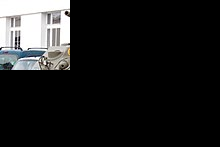
\includegraphics[width=0.14\textwidth]{img/czolg_masked_1.png}};
\node at (2,-1.5) {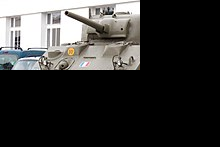
\includegraphics[width=0.14\textwidth]{img/czolg_masked_2.png}};
\node at (4,-1.5) {$\dots$};
\node at (6,-1.5) {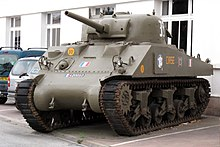
\includegraphics[width=0.14\textwidth]{img/czolg.jpg}};

\end{tikzpicture}
\end{center}
\end{minipage}
    \hrule
    \pause
    \begin{center}
    \textbf{Normalizing Flows} \\
    \begin{tikzpicture}
        \node[rand_var, inner sep=5pt] (z0) at (-1,0) {$z_0$};
        \node[rand_var, inner sep=5pt] (z1) at (1,0) {$z_1$};
        \node[rand_var, inner sep=5pt] (z2) at (3,0) {$z_2$};
        \node[inner sep=5pt] (dots) at (5,0) {$\ldots$};
        \node[rand_var, inner sep=5pt] (zk) at (7,0) {$z_k$};
        \draw[->] (z0) to node[above] {$f_1(z_0)$} (z1);
        \draw[->] (z1) to node[above] {$f_2(z_1)$} (z2);
        \draw[->] (z2) to node[above] {$f_3(z_2)$} (dots);
        \draw[->] (dots) to node[above] {$f_k(z_{k-1})$} (zk);
        % gaussian distribution and transformed ones
            \begin{scope}[shift={(-1,-0.75)},scale=0.075]
        \begin{axis}[
            anchor=center,
            domain=-3:3,
            samples=100,
            height=10cm,
            width=10cm,
            yticklabels={,,},
            xticklabels={,,},
            xmin=-3, xmax=3,
            ymin=0, ymax=0.5
        ]
        \addplot[smooth, very thick, blue] {1/sqrt(2*pi) * exp(-x^2/2)};
        \end{axis}
    \end{scope}
    % first trafo:
    \begin{scope}[shift={(1,-0.75)},scale=0.075]
        \begin{axis}[
            anchor=center,
            domain=-3:3,
            samples=100,
            height=10cm,
            width=10cm,
            yticklabels={,,},
            xticklabels={,,},
            xmin=-3, xmax=3,
            ymin=0, ymax=0.5
        ]
        \addplot[smooth, very thick, blue]  
        {0.5*(1/sqrt(0.5*2*pi) * exp(-(x+0.5)^2/(2*0.5^2))) 
        + 0.5*(1/sqrt(0.7*2*pi) * exp(-(x-1)^2/(2*0.7^2)))};
        \end{axis}
    \end{scope}
    % second trafo:
    \begin{scope}[shift={(3,-0.75)},scale=0.075]
        \begin{axis}[
            anchor=center,
            domain=-3:3,
            samples=100,
            height=10cm,
            width=10cm,
            yticklabels={,,},
            xticklabels={,,},
            xmin=-3, xmax=3,
            ymin=0, ymax=0.5
        ]
        \addplot[smooth, very thick, blue]  
        {0.3*(1/sqrt(0.3*2*pi) * exp(-(x+0.25)^2/(2*0.3^2))) 
        + 0.2*(1/sqrt(0.15*2*pi) * exp(-(x+1.15)^2/(2*0.15^2))) 
        + 0.5*(1/sqrt(0.7*2*pi) * exp(-(x-1)^2/(2*0.7^2)))};
        \end{axis}
    \end{scope}
    \node at (5,-0.75) {$\dots$};
   % final distribution:
    \begin{scope}[shift={(7,-0.75)},scale=0.075]
        \begin{axis}[
            anchor=center,
            domain=-3:3,
            samples=100,
            height=10cm,
            width=10cm,
            yticklabels={,,},
            xticklabels={,,},
            xmin=-3, xmax=3,
            ymin=0, ymax=0.5
        ]
        \addplot[smooth, very thick, blue] 
        {0.3*(1/sqrt(0.3*2*pi) * exp(-(x+0.25)^2/(2*0.3^2))) 
        + 0.2*(1/sqrt(0.15*2*pi) * exp(-(x+1.15)^2/(2*0.15^2))) 
        + 0.15*(1/sqrt(0.4*2*pi) * exp(-(x-2.1)^2/(2*0.4^2)))
        + 0.35*(1/sqrt(0.2*2*pi) * exp(-(x-0.9)^2/(2*0.2^2)))};
        \end{axis}
    \end{scope}
        \end{tikzpicture}
    \end{center}
    \hrule
    \pause
    \begin{center}
    \textbf{Diffusion Model} (a.k.a.\ Markovian Hierarchical Variational Autoencoder)
    % generate noisy images
%    \immediate\write18{python3 img/noise_image.py img/SuperMario.png img/SuperMario_noise_40.png 40}
%    \immediate\write18{python3 img/noise_image.py img/SuperMario.png img/SuperMario_noise_80.png 80}
%    \immediate\write18{python3 img/noise_image.py img/SuperMario.png img/SuperMario_noise_100.png 100}
    \begin{tikzpicture}
        \node[rand_var, inner sep=5pt] (x) at (-1,0) {$x$};
        \node[rand_var, inner sep=5pt] (z1) at (1,0) {$z_1$};
        \node[rand_var, inner sep=5pt] (z2) at (3,0) {$z_2$};
        \node[inner sep=5pt] (dots) at (5,0) {$\ldots$};
        \node[rand_var, inner sep=5pt] (zT) at (7,0) {$z_T$};
        \draw[->, bend left=45] (x) to node[above] {$q(z_1|x)$} (z1);
        \draw[->, bend left=45] (z1) to node[above] {$q(z_2|z_1)$} (z2);
        \draw[->, bend left=45] (z2) to node[above] {$q(z_3|z_2)$} (dots);
        \draw[->, bend left=45] (dots) to node[above] {$q(z_{T}|z_{T-1})$} (zT);
        \draw[->, bend left=45] (zT) to node[below] {$p(z_{T-1}|z_T)$} (dots);
        \draw[->, bend left=45] (dots) to node[below] {$p(z_2|z_3)$} (z2);
        \draw[->, bend left=45] (z2) to node[below] {$p(z_1|z_2)$} (z1);
        \draw[->, bend left=45] (z1) to node[below] {$p(x|z_1)$} (x);
        
        \node at (-1,-1) {\includegraphics[width=0.05\textwidth]{img/SuperMario.png}};
        \node at (1,-1) {\includegraphics[width=0.05\textwidth]{img/SuperMario_noise_40.png}};
        \node at (3,-1) {\includegraphics[width=0.05\textwidth]{img/SuperMario_noise_80.png}};
        \node at (5,-1) {$\dots$};
        \node at (7,-1) {\includegraphics[width=0.05\textwidth]{img/SuperMario_noise_100.png}};
        \end{tikzpicture}
    \end{center}
\end{frame}

\begin{frame}{Deep Learning vs.\ PML}
\begin{center}
\begin{tabular}{|>{\columncolor{gray!30}}p{0.15\textwidth}|p{0.33\textwidth}|p{0.33\textwidth}|}
    \hline
    \rowcolor{gray!30}
& \textbf{Deep Learning} & \textbf{Probabilistic Machine Learning} \\ \hline
\textbf{Goals} & Classification, feature learning, regression & Sampling, infering latent variables \\ \hline
\pause
\textbf{Vocabulary} & Neurons, activations, layers, $\ldots$ & Random variables, potentials \\ \hline
\pause
\textbf{Mathematical technique} & Differentiating & Sampling, marginalizing, differentiating \\ \hline
\pause
\textbf{Inference} & Simple forward pass & Monte-Carlo, belief propagation, message passing, linear programming, dynamic programming, $\ldots$ \\ \hline
\pause
\textbf{Learning} & Backprop \& gradient descent & MLE, EM, ELBO, $\ldots$ \\ \hline
\pause
\textbf{Impementation} & Many tricks to make it work & More standardized? \\ \hline
\end{tabular}
\pause
\vspace{0.1cm}

\textbf{Wisdom:} use DL + probabilistic techniques!\\
\vspace{0.2cm}

\includegraphics[width=0.3\textwidth]{img/dl+pml=generative.jpeg}\\
\end{center}
\end{frame}

\begin{frame}{PGM Lecture Overview}
\begin{minipage}{0.49\textwidth}
\begin{itemize}
    \item Bayesian (Directed) Graphical Models
    \begin{itemize}
    \item Conditional Independence, Factorization, Separation
    \end{itemize}
    \item Undirected (Markov) Graphical Models
    \item Inference in PGMs
    \begin{itemize}
        \item Exact
        \item Approximate: Monte-Carlo \& Variational
    \end{itemize}
    \item Learning PGMs
    \begin{itemize}
    \item MLE
    \item Expectation-Maximization
    \end{itemize}
\end{itemize}
\end{minipage}
\begin{minipage}{0.49\textwidth}
\begin{itemize}
    \item Autoregressive Models
    \item VAEs 
    \item Normalizing Flows
    \item Diffusion Models
\end{itemize}
\end{minipage}
\end{frame}

%\section{Bayesian Networks}

\begin{frame}{Bayesian Networks: Introduction}
    \begin{itemize}
        \item The probability distribution is factorized according to a directed acyclic graph.
        \pause \item Conditional independency assumptions hold according to graph topology.
        \pause \item Sampling can be done efficiently by traversing the graph.
        \pause \item Representation is more compact than storing a full array if graph is sparse.
    \end{itemize}
        \pause
        \hrule
        \begin{minipage}[t]{0.49\textwidth}
        \textbf{Example:} Antique Greek Poleis
        \begin{center}
        \begin{tikzpicture}[scale=0.5]
            \node [rand_var] (0) at (-2, 5) {P: Prosperity};
            \node [rand_var] (1) at (2, 3) {F: Fighting Spirit};
            \node [rand_var] (2) at (0, 0) {W: War Success};
            \node [rand_var] (4) at (0, -2) {E: Everlasting Fame};
            \node [rand_var] (3) at (-5, 2) {C: Culture};
            \draw[->] (0) to (3);
            \draw[->] (0) to (2);
            \draw[->] (1) to (2);
            \draw[->] (2) to (4);
            \draw[->] (0) to (1);
            \draw[->, bend right=10] (3) to (4);
        \end{tikzpicture}
    \end{center}
\end{minipage}
    \pause
    \hfill\vrule\hfill
        \begin{minipage}[t]{0.49\textwidth}
            \textbf{Example:} Hidden Markov Model (HMM)
            \begin{center}
                \begin{tikzpicture}[scale=0.5]
                        \node[rand_var] (0) at (-9, 3) {$X_1$};
                        \node[rand_var] (1) at (-9, 1) {$Y_1$};
                        \node[rand_var] (2) at (-7, 3) {$X_2$};
                        \node[rand_var] (3) at (-7, 1) {$Y_2$};
                        \node[rand_var] (4) at (-5, 3) {$X_3$};
                        \node[rand_var] (5) at (-5, 1) {$Y_3$};
                        \node[rand_var] (6) at (-3, 3) {$X_4$};
                        \node[rand_var] (7) at (-3, 1) {$Y_4$};
                        \node[rand_var] (8) at (-1, 3) {$X_5$};
                        \node[rand_var] (9) at (-1, 1) {$Y_5$};
                        \node[rand_var] (10) at (1, 3) {$X_6$};
                        \node[rand_var] (11) at (1, 1) {$Y_6$};
                        \draw[->] (0) to (1);
                        \draw[->] (0) to (2);
                        \draw[->] (2) to (4);
                        \draw[->] (4) to (6);
                        \draw[->] (6) to (8);
                        \draw[->] (8) to (10);
                        \draw[->] (2) to (3);
                        \draw[->] (4) to (5);
                        \draw[->] (6) to (7);
                        \draw[->] (8) to (9);
                        \draw[->] (10) to (11);
                \end{tikzpicture}
            \end{center}
                \vspace{0.2cm}
                \begin{itemize}
                    \pause \item $X_i$ are the true but hidden states of a system.
                    \pause \item $Y_i$ are the observations (or measurements), from which one can partially infer the states.
                    \pause \item $X_i$ evolves through time.
                    \pause \item \textbf{Example:} Speech recognition, Kalman filters, $\ldots$
                \end{itemize}
\end{minipage}
\end{frame}

\subsection{Definitions, I-Map, Factorization}
\begin{frame}{Definitions: Bayesian Network Structure, I-Map}
\begin{definition}[Bayesian Network Structure, $\Indep_l$]
    A Bayesian network structure is a directed acyclic graph $G = (V,A)$ whose nodes represent random variables $X_1,\ldots, X_n$.
    Let $\Pa{G}{X_i}$ be the parents of $X_i$ in $G$.
    Let $\ND{G}{X_i}$ be the nodes that are not descendants of $X_i$ in $G$.
    Then $G$ encodes the following local conditional independence relations:
    \begin{equation}
X_i \indep \ND{G}{X_i} \backslash \Pa{G}{X_i} | \Pa{G}{X_i}
    \end{equation}
    We call these relations $\Indep_l(G)$.
\end{definition}
\pause
\begin{itemize}
    \item \textbf{Short:} Each variable is conditionally independent of its non-descendants, given its parents.
\end{itemize}
    \pause
\begin{definition}[Independence of Distribution]
    Let $\Pb$ be a probability distribution over a set of variables.
    We define $\Indep(\Pb)$ to be the set of independence relations of the form $X \indep Y | Z$ that hold for $\Pb$.
\end{definition}
    \pause
\begin{definition}[I-map]
    We say that $G=(V,E)$ is an I-map for a probability distribution $\Pb$ if $\Indep_l(G) \subseteq \Indep(\Pb)$.
\end{definition}
\begin{itemize}
\item Distribution has more independencies than graph
\item Graph does not mislead independencies in $\Pb$
\end{itemize}
\end{frame}

\begin{frame}{Factorization}
    \begin{definition}[Factorization]
        Let $G$ be an directed graph whose nodes are random variables $X_1,\ldots,X_n$.
        We say that the corresponding probability distribution $\Pb$ factorizes over $G$ if 
        \begin{equation}
            \Pb[X_1,\ldots,X_n] = \prod_{i=1}^n \Pb[X_i | \Pa{G}{X_i}]
        \end{equation}
    \end{definition}
    \pause
    \begin{definition}[Bayesian Network]
     A Bayesian network is a pair $B = (G,\Pb)$ such that $\Pb$ factorizes over $G$. 
     %Given $B$ we write $\Pb_B$ to denote the corresponding probability distribution.
    \end{definition}
    \pause
    \begin{example}[Chain Graph]
        \begin{tikzpicture}[baseline=(1.base),scale=0.8]
        \node[rand_var] (1) at (0,0) {$X_1$};
        \node[rand_var] (2) at (1,0) {$X_2$};
        \node[rand_var] (3) at (2,0) {$X_3$};
        \node[rand_var] (4) at (3,0) {$X_4$};
        \node[rand_var] (5) at (4,0) {$X_5$};
        \node[rand_var] (6) at (5,0) {$X_6$};
        \draw[->] (1) to (2);
        \draw[->] (2) to (3);
        \draw[->] (3) to (4);
        \draw[->] (4) to (5);
        \draw[->] (5) to (6);
        \end{tikzpicture}
        factorizes as $\Pb[X_1,\ldots,X_6] = \Pb[X_1] \cdot \Pb[X_2 | X_1] \cdots \Pb[X_6 | X_5]$.
    \end{example}
    \pause 
    \begin{example}[Autoregressive Model]
\begin{tikzpicture}[baseline=(x1.base),scale=0.4]
\node[rand_var] (x1) at (0,0) {${X_1}$};
\node[rand_var] (x2) at (2,0) {${X_2}$};
\node[inner sep=5pt] (dots) at (4,0) {$\ldots$};
\node[rand_var] (xk) at (6,0) {${X_k}$};
\draw[->] (x1) -- (x2);
\draw[->] (x2) -- (dots);
\draw[->] (dots) -- (xk);
\draw[->, bend left=30] (x1) to (xk);
\draw[->, bend left=20] (x2) to (xk);
\end{tikzpicture}
factorizes as
        $\Pb[X_1,X_2,\ldots,X_k] = \Pb[X_1] \Pb[X_2 | X_1] \cdots \Pb[X_k | X_1,\ldots,X_{k-1}]$
    \end{example}
    \end{frame}

\begin{frame}{I-map $\Rightarrow$ Factorization}
\begin{theorem}
    Let $G$ be a Bayesian network structure and let $\Pb$ be a probability distribution over the set of nodes of $G$. If $G$ is an I-map for $\Pb$, then $\Pb$ factorizes over $G$ (i.e.\ it is a Bayesian network).
    \end{theorem}
    \pause
    \begin{proof}
    Let $X_1,\ldots,X_n$ be the random variables ordered topologically w.r.t.\ $G$.
    \pause
    Rewrite autoregressively
    \begin{equation}
    \Pb[X_1,X_2,\ldots,X_k] = \Pb[X_1] \Pb[X_2 | X_1] \ldots \Pb[X_k | X_1,\ldots,X_{k-1}]
    \end{equation}
    \pause
    As $G$ is an I-map for $\Pb$, we have that
    \pause
    $(X_i \indep \ND{G}{X_i} \backslash \Pa{G}{X_i} | \Pa{G}{X_i}) \in \Indep(P)$.
    \pause
    By assumption, all parents of $X_i$ are in the set $X_1,\ldots,X_{i-1}$.
    \pause
    None of the descendants can possibly be in the same set.
    \pause
    Hence, choose $Z \subseteq \ND{G}{X_i}$ such that $Z \cup \Pa{G}{X_i} = \{X_1,\ldots,X_{i-1}\}$.
    \pause
    From the local independence for $X_i$ and from decomposition it follows that $(X_i \indep Z | \Pa{G}{X_i})$.
    \pause
    Hence, by Bayes rule
    \begin{equation}
\Pb[X_i | X_1,\ldots,X_{i-1}]
%\Pb[X_i | Z, \Pa{G}{X_i}]
= \frac{\Pb[X_i,Z | \Pa{G}{X_i}]}{\Pb[Z | \Pa{G}{X_i}]}
\pause
= \frac{\Pb[X_i | \Pa{G}{X_i}] \Pb[Z | \Pa{G}{X_i}]}{\Pb[Z | \Pa{G}{X_i}]}
\pause
= \Pb[X_i | \Pa{G}{X_i}]
    \end{equation}
    \pause
    Rewrite the autoregressive formulation using the above formula.
    \end{proof}
    \end{frame}

    \begin{frame}{Factorization $\Rightarrow$ I-map}
    \begin{theorem}
    Let $G$ be a Bayesian network structure and let $\Pb$ be a probability distribution over the set of nodes of $G$.
    If $\Pb$ factorizes over $G$, then $G$ is an I-map for $\Pb$.
    \end{theorem}
    \pause
    First, we need a technical lemma.
    \begin{lemma}
        \label{lemma:Bayesian-network-restriction}
    Let $\Pb$ factorize over a graph $G$. then
    \begin{equation}
    \Pb[X_i, \ND{G}{X_i}] = \prod_{j \in \{i\} \cup \ND{G}{X_i}} \Pb[X_j | \Pa{G}{X_j}]
    \end{equation}
    \end{lemma}
    \pause
    \begin{proof}
        We proceed by induction.
        If $\Desc{X_i} \neq \varnothing$, there is necessarily a leaf node $X_j \in \Desc{X_i}$.
        \pause
        We use that in the factorization $\Pb[X_1,\ldots,X_n] = \prod_{i} \Pb[X_i | \Pa{G}{X_i}]$ the variable $X_j$ appears exactly once in $\Pb[X_j | \Pa{G}{X_j}]$. 
        \pause
        We marginalize $X_j$ out and obtain
        \begin{equation}
            \Pb[X_{i \neq j}] = 
            \pause  \sum_{X_j} \prod_{i \neq j} \Pb[X_i | \Pa{G}{X_i}] \Pb[X_j | \Pa{G}{X_j}]
            = \pause \prod_{i \neq j} \Pb[X_i | \Pa{G}{X_i}] \,.
        \end{equation}
        \pause
        This solves the induction step.
    \end{proof}
    \end{frame}

    \begin{frame}{Factorization $\Rightarrow$ I-map, proof}
    \begin{proof}[Factorization $\rightarrow$ I-Map]
    Let $\Pb$ be a distribution that factorizes according to $G$.
    We need to show that $\Indep_l(G)$ holds in $\Pb$.
    \pause
    Let $(X_i \indep \ND{G}{X_i} \backslash \Pa{G}{X_i}| \Pa{G}{X_i})$ be an independence relation in $G$.
    \pause
    To prove that it holds for $\Pb$, we need to show that
    \begin{equation}
        \Pb[X_i | \ND{G}{X_i} ] = \Pb[X_i | \Pa{G}{X_i}] 
    \end{equation}
    \pause
    First, let us assume that $X_i$ is a leave node (i.e.\ has no descendants).
    Then 
    \begin{equation}
        \label{eq:def-xi-nd}
        \Pb[X_{j \neq i}] = \pause \sum_{X_i} \prod_{j \neq i}\Pb[X_j| \ND{G}{X_j}] \Pb[X_i | \Pa{G}{X_i}] = \pause \prod_{j \neq i}\Pb[X_j| \ND{G}{X_j}]\,.
    \end{equation}
    \pause
    Hence,
    \begin{equation}
    \Pb[X_i | \ND{G}{X_i}] = \frac{\Pb[X_i | \Pa{G}{X_i}] \prod_{j \neq i}\Pb[X_j| \ND{G}{X_j}]}{\prod_{j \neq i} \Pb[X_j| \ND{G}{X_j}] } = \Pb[X_i | \Pa{G}{X_i}] 
    \end{equation}

    \pause
    In the general case when $X_i$ is not a leave node, we apply the lemma to marginalize out all $X \in \Desc{X_i}$ and follow the reasoning in the leave case.
\end{proof}
\end{frame}

\subsection{D-Separation}
\begin{frame}{D-Separation, Elementary Examples}
\begin{center}
\textbf{When does $X \indep Y | Z$ hold given in a BN?}
\end{center}
\pause
\hrule
\begin{minipage}[t]{0.3\textwidth}
\textbf{Direct Effect:}
        \begin{tikzpicture}[baseline=(0.base)]
            \node[rand_var] (0) at (-1, 0) {$X$};
            \node[rand_var] (1) at (0, 0) {$Y$};
            \draw[->] (0) to (1);
        \end{tikzpicture}
        \begin{itemize}
        \item $X \indep Y$? \pause No 
        \end{itemize}
    \end{minipage}
    \hfill\vrule\hfill
    \begin{minipage}[t]{0.69\textwidth}
\pause \textbf{Indirect Effect, Causal Chain:}
        \begin{tikzpicture}[baseline=(0.base)]
            \node[rand_var] (0) at (-1, 0) {$X$};
            \node[rand_var] (1) at (0, 0) {$Z$};
            \node[rand_var] (2) at (1, 0) {$Y$};
            \draw[->] (0) to (1);
            \draw[->] (1) to (2);
        \end{tikzpicture}
        \begin{itemize}
        \item $X\indep Y$? \pause No 
        \pause \item $X \indep Y | Z$? \pause Yes
        \end{itemize}
        \pause
        \begin{equation}
        \Pb[Y|X,Z] = \frac{\Pb[X,Y,Z]}{\Pb[X,Z]} = \frac{\Pb[X] \Pb[Z|X] \Pb[Y|Z]}{\Pb[X]\Pb[Z|X]} = \Pb[Y|Z]
        \end{equation}
    \end{minipage}
    \hrule
    \begin{minipage}[t]{0.47\textwidth}
\pause \textbf{Common Cause:}
        \begin{tikzpicture}[baseline=(b.base)]
            \node (b) at (0,0.3) {};
            \node[rand_var] (0) at (0, 0.6) {$Z$};
            \node[rand_var] (1) at (-0.75, 0) {$X$};
            \node[rand_var] (2) at (0.75, 0) {$Y$};
            \draw[->] (0) to (1);
            \draw[->] (0) to (2);
        \end{tikzpicture}
        \begin{itemize}
        \pause \item $X \indep Y$: \pause No
        \pause \item $X \indep Y | Z$: \pause Yes
        \end{itemize}
        \pause
        \begin{equation}
        \Pb[Y | Z,X] = \frac{\Pb[Z] \Pb[X|Z] \Pb[Y|Z]}{\Pb[Z] \Pb[X|Z]} = \Pb[Y|Z]
        \end{equation}
    \end{minipage}
    \hfill\vrule\hfill
    \begin{minipage}[t]{0.52\textwidth}
\pause \textbf{Common Effect, v-structure:}
        \begin{tikzpicture}[baseline=(b.base)]
            \node (b) at (0,0.3) {};
            \node[rand_var] (0) at (0, 0) {$Z$};
            \node[rand_var] (1) at (-0.75, 0.6) {$X$};
            \node[rand_var] (2) at (0.75, 0.6) {$Y$};
            \draw[->] (1) to (0);
            \draw[->] (2) to (0);
        \end{tikzpicture}
        \begin{itemize}
            \pause \item $X \indep Y$: \pause Yes
        \end{itemize}
        \pause
        \begin{multline}
        \Pb[Y | X] = \frac{\Pb[X,Y]}{\Pb[X]} \\ = \frac{\sum_{Z} \Pb[X] \Pb[Y] \Pb[Z=z|X,Y]}{\Pb[X]} = \Pb[Y]
        \end{multline}
        \begin{itemize}
            \pause \item $X \indep Y | Z$: \pause No, counterexample possible
        \end{itemize}
        \pause
        \begin{equation}
        \Pb[Y | Z,X] = \frac{\Pb[X] \Pb[Y] \Pb[Z|X,Y]}{\sum_{Y}\Pb[X] \Pb[Y=y] \Pb[Z|X,Y=y]} = ?
        \end{equation}
        \pause
        Counterexample possible
    \end{minipage}
\end{frame}

\begin{frame}{Active Trail, D-Separation}
\begin{columns}
    \column{0.5\textwidth}
\textbf{General case:} Query $X \indep Y | Z$?\\
\begin{itemize}
\pause \item Check all trails (= undirected paths) between pairs of nodes in $X$ and $Y$.
\pause \item On the trail check all triplets:
\begin{itemize}
    \pause \item $A \rightarrow B \rightarrow C$ and $B \notin Z$ 
        $\Rightarrow$ $\surd$
    \pause \item $A \leftarrow B \rightarrow C$ and $B \notin Z$ 
        $\Rightarrow$ $\surd$
    \pause \item $A \rightarrow B \leftarrow C$ and $(B \cup \Desc{B}) \cap Z = \varnothing$ 
        $\Rightarrow$ $\surd$
\end{itemize}
\pause \item If all checks are positive, the \underline{trail is active} and the query \underline{cannot} be answered positively.
\pause \item Intuition active trail: Information can flow from $X_1$ to $X_n$.
\end{itemize}
\pause
\begin{definition}[D-Separation]
$X$ and $Y$ are d-separated given $Z$ if there is no active trail between them.
$\mathcal{I}(G)$ denotes the set of independencies that correspond to d-separation:
\begin{equation}
    \mathcal{I}(G) := \left\{ X \indep Y | Z: \begin{array}{l} X \text{ and } Y \text{ d-separated} \\ \text{given } Z \end{array} \right\}
\end{equation}
\end{definition}
    \pause
    \column{0.5\textwidth}
    \begin{center}
\begin{tikzpicture}
\tikzset{ X/.style = {rectangle, fill=blue!50, inner sep=0.25cm} }
\tikzset{ Y/.style = {rectangle, fill=green!50, inner sep=0.25cm} }
\tikzset{ Z/.style = {rectangle, fill=red!50, inner sep=0.25cm} }
    % node pos
    \node (A) at (0,0) {};
   \node (B) at (-0.5,-1) {};
   \node (C) at (0,-2) {};
   \node (D) at (1,-0.5) {};
   \node (E) at (1,-1.5) {};
   \node (F) at (1,-2.5) {};
   \node (G) at (2,0) {};
   \node (H) at (2,-2) {};
   \node (I) at (3,-3) {};
   \node (J) at (3,-3) {};
    % queries
    \only<10>{
\node[X] at (A) {};
\node[Y] at (G) {};
    }
    \only<11>{
\node[X] at (A) {};
\node[Y] at (G) {};
\node[Z] at (D) {};
\node[Z] at (C) {};
    }
    \only<12>{
\node[X] at (A) {};
\node[Y] at (G) {};
\node[Z] at (E) {};
\node[Z] at (C) {};
    }
    \only<13>{
\node[X] at (A) {};
\node[Y] at (G) {};
\node[Z] at (F) {};
\node[Z] at (J) {};
    }
   % random vars
   \node[rand_var] (A_node) at (A) {$A$};
   \node[rand_var] (B_node) at (B) {$B$};
   \node[rand_var] (C_node) at (C) {$C$};
   \node[rand_var] (D_node) at (D) {$D$};
   \node[rand_var] (E_node) at (E) {$E$};
   \node[rand_var] (F_node) at (F) {$F$};
   \node[rand_var] (G_node) at (G) {$G$};
   \node[rand_var] (H_node) at (H) {$H$};
   \node[rand_var] (I_node) at (I) {$I$};
   \node[rand_var] (J_node) at (J) {$J$};
   %
   \draw[->] (A_node) -- (B_node);
   \draw[->] (A_node) -- (D_node);
   \draw[->] (B_node) -- (C_node);
   \draw[->] (C_node) -- (F_node);
   \draw[->] (D_node) -- (E_node);
   \draw[->] (G_node) -- (D_node);
   \draw[->] (G_node) -- (H_node);
   \draw[->] (H_node) -- (F_node);
   \draw[->] (H_node) -- (J_node);
   % legend
   \node at (-0.5,-4) {$X$:};
   \node[X] at (0,-4) {};
   \node at (1.0,-4) {$Y$:};
   \node[Y] at (1.5,-4) {};
   \node at (2.5,-4) {$Z$:};
   \node[Z] at (3,-4) {};
\end{tikzpicture}
\end{center}
\end{columns}
\end{frame}

\begin{frame}{D-Separation}
    \label{slide:d-separation}
\begin{theorem}[Soundness of d-separation]
    If a distribution $\Pb$ factorizes according to $G$, then $\mathcal{I}(G) \subseteq \mathcal{I}(\Pb)$.
\end{theorem}
\pause
\begin{itemize}
    \item Proof will be given later in the lecture (need more tools).
\end{itemize}
\pause
\begin{theorem}[Completeness]
Let $G$ be a BN-structure. If $X$ an $Y$ are not d-separated given $Z$, then $X$ and $Y$ are dependent given $Z$ in some distribution  $\Pb$ that factorizes according to $G$.
\end{theorem}
\pause
\begin{proof}
    By construction.
    As $X$ and $Y$ are not d-separated, there exists an active trail $U_1 \rightleftarrows \ldots \rightleftarrows U_k$ between them.
    We choose conditional probability distributions on the trail to make each $U_i, U_{i+1}$ correlated.
    \pause
    For $U_{i} \rightarrow U_{i+1} \leftarrow U_{i+2}$ we define the distribution of $U_{i+1}$ to be correlated to both $U_{i}$ and $U_{i+2}$.
    Additionally, descendant nodes also activate correlation between $U_i$ and $U_{i+2}$.
    \pause 
    All other random variables are assumed to be independent.
    \pause 
    Thus, correlation only is contributed through the considered path and cannot cancel out.
    \pause Technical details are laborious and we omit them here.
    
\end{proof}
\end{frame}

\begin{frame}{D-Separation Algorithm}
\textbf{Problem:} Enumerating all trails and checking for d-separation is exponential time! \\
\textbf{Solution:} Efficient polynomial algorithm possible:
\begin{description}
\pause \item[Phase I:] Bottom-Up Traversal for Marking $Z$.
\begin{itemize}
\pause \item From all leaves to roots, mark all nodes that are in $Z$ or that have descendants in $Z$.
\pause \item Remember for identifying activity in v-structures.
\end{itemize}
\pause \item[Phase II:] Breadth-First Search for Blocking Node Identification.
\begin{itemize}
    \pause \item Traverse from $X$ to $Y$ breadth-first.
    \pause \item Stop if:
\begin{itemize}
    \item Node is in middle of v-structure and not marked in previous phase,
    \item Is not in middle of v-structure and in $Z$,
\end{itemize}
    \pause \item Else if reached $Y$: Trail is active.
\end{itemize}
\end{description}
%\end{frame}
\pause
\color{gray!90}
%\begin{frame}{D-Separation Algorithm Phase I}
\begin{algorithm}[H]
\caption{D-Separation Phase I}
\KwData{Input: $G$, $X$, $Y$, $Z$}
\tcp{Insert all ancestors of $Z$ into $L$}
$L \leftarrow Z$ \tcp{Nodes to be visited}
$A \leftarrow \varnothing$ \tcp{Ancestors of $Z$}
\While{$L \neq \varnothing$}
{
Select some node $W$ from $L$\;
$L \leftarrow L\backslash \{W\}$\;
\If{$W \notin A$}
{
    $L \leftarrow L \cup \Pa{G}{W}$\;
    $A \leftarrow A \cup \{W\}$\;
}
}
\end{algorithm}
\end{frame}

\begin{frame}{D-Separation Algorithm Phase II}
\color{gray!90}
\begin{algorithm}[H]
\caption{D-Separation Phase II}
\KwData{Input: $G$, $X$, $Y$, $Z$ $A$}
$L \leftarrow \{(X,\uparrow)\}$ \tcp{Node \& direction to be visited}
$V \leftarrow \varnothing$ \tcp{Node \& direction marked as visited}
$R \leftarrow \varnothing$ \tcp{Nodes reachable via active trail}
\While{$L \neq \varnothing$}
{
    Select some $(W,d)$ from $L$, $L \leftarrow L \backslash \{(W,d)\}$\;
    \If{$(W,d) \notin V$}
    {
    \If{$W \notin Z$}
    {
        $R \leftarrow R \cup \{W\}$ \tcp{$W$ is reachable}
    }
    $V \leftarrow V \cup \{(W,d)\}$ \tcp{Mark $(W,d)$ as visited}
    \If{$d = \uparrow$ and $W \notin Z$}
    {
        \For{$U \in \Pa{G}{W}$}
        {
            $L \leftarrow L \cup \{(U,\uparrow)\}$\;
        }
        \For{$U \in \Ch{G}{W}$}
        {
            $L \leftarrow L \cup \{(U,\downarrow)\}$\;
        }
    } 
    \ElseIf{$d = \downarrow$}
    {
    \If{$W  \notin Z$}
    {
        \For{$U \in \Ch{G}{W}$}
        {
            $L \leftarrow L \cup \{(U,\downarrow)\}$
        }
        \If{$W \in A$}
        {
            \For{$U \in \Pa{G}{W}$}
            {
                $L \leftarrow L \cup \{(U,\uparrow)\}$
            }
        }
    }
    }
    }
}
Test $Y \in R$\;
\end{algorithm}
\end{frame}

\begin{frame}{Equivalent I-Maps}
\begin{itemize}
\item Different graphs can encode the same independencies.
\end{itemize}
\begin{center}
\begin{tikzpicture}[baseline=(0.base)]
    \node[rand_var] (0) at (-1, 0) {$X$};
    \node[rand_var] (1) at (0, 0) {$Z$};
    \node[rand_var] (2) at (1, 0) {$Y$};
    \draw[->] (0) to (1);
    \draw[->] (1) to (2);
\end{tikzpicture}
\hfill
\begin{tikzpicture}[baseline=(0.base)]
    \node[rand_var] (0) at (-1, 0) {$X$};
    \node[rand_var] (1) at (0, 0) {$Z$};
    \node[rand_var] (2) at (1, 0) {$Y$};
    \draw[<-] (0) to (1);
    \draw[<-] (1) to (2);
\end{tikzpicture}
\hfill
\begin{tikzpicture}[baseline=(0.base)]
    \node[rand_var] (0) at (-1, 0) {$X$};
    \node[rand_var] (1) at (0, 0) {$Z$};
    \node[rand_var] (2) at (1, 0) {$Y$};
    \draw[<-] (0) to (1);
    \draw[->] (1) to (2);
\end{tikzpicture}
\end{center}
\pause
\begin{definition}[I-Equivalence]
    Two graph structures $G_1$ and $G_2$ are I-equivalent if $\Indep(G_1) = \Indep(G_2)$.
\end{definition}
\pause
\begin{definition}[Skeleton]
   The skeleton of a Bayesian network $G$  is an undirected graph that contains an edge $\{X,Y\}$ for every arc $(X,Y)$ in $G$.
\end{definition}
\pause
\begin{itemize}
    \item $G_1$ and $G_2$ have the same skeleton $\overset{?}{\Rightarrow}$ $G_1$ and $G_2$ are $I$-equivalent. \pause No
\end{itemize}
\pause
\begin{theorem}[I-Equivalence]
Let $G_1$ and $G_2$ be two directed acyclic graphs.
If $G_1$ and $G_2$ have the same skeleton and the same set of v-structures then they are I-equivalent.
\end{theorem}
\pause
\begin{proof}
    Follows from the characterization of d-separation in terms of v-structures and active trails.
\end{proof}
\end{frame}

\begin{frame}{Immoralities}
    \begin{itemize}
    \item Are graphs I-equivalent?
    \end{itemize}
    \begin{center}
    \begin{tikzpicture}[scale=0.7]
    \node[rand_var] (X) at (-1,0) {$X$};
    \node[rand_var] (Z) at (0,-1.15) {$Z$};
    \node[rand_var] (Y) at (1,0) {$Y$};
    \draw[thick,->] (X) -- (Z);
    \draw[thick,->] (Y) -- (Z);
%
    \begin{scope}[shift={(4,0)}]
    \node[rand_var] (X) at (-1,0) {$X$};
    \node[rand_var] (Z) at (0,-1.15) {$Z$};
    \node[rand_var] (Y) at (1,0) {$Y$};
    \draw[thick,->] (X) -- (Z);
    \draw[thick,->] (Y) -- (Z);
    \draw[thick,->] (X) -- (Y);
    \end{scope}
\pause
    \begin{scope}[shift={(8,0)}]
    \node[rand_var] (X) at (-1,0) {$X$};
    \node[rand_var] (Z) at (0,-1.15) {$Z$};
    \node[rand_var] (Y) at (1,0) {$Y$};
    \draw[thick,->] (X) -- (Z);
    \draw[thick,->] (Y) -- (Z);
    \draw[thick,<-] (X) -- (Y);
    \end{scope}
\pause
    \begin{scope}[shift={(12,0)}]
    \node[rand_var] (X) at (-1,0) {$X$};
    \node[rand_var] (Z) at (0,-1.15) {$Z$};
    \node[rand_var] (Y) at (1,0) {$Y$};
    \draw[thick,<-] (X) -- (Z);
    \draw[thick,->] (Y) -- (Z);
    \draw[thick,<-] (X) -- (Y);
    \end{scope}
    \end{tikzpicture}
\end{center}
    \pause
\begin{definition}[Immorality]
    A v-structure $X \rightarrow Z \leftarrow Y$ is an immorality if there is no arc between $X$ and $Y$.
\end{definition}
\pause
\begin{theorem}[I-Equivalence II]
    $G_1$ and $G_2$ are I-equivalent iff they have the same skeleton and the same set of immoralities.
\end{theorem}
\begin{proof}
Skipped.
\end{proof}
\end{frame}
%\section{Markov/Undirected Graphical Models}

\begin{frame}{Gibbs Distribution}
\begin{definition}[Factor, Clique Potential]
    Let $\mathcal{S} \subseteq \mathcal{X} = (X_1,\ldots,X_n)$ be a set of random variables with label spaces $L_{X_1},\ldots,L_{X_n}$.
    We define a factor (also called clique potential) $\phi$ to be a function from $\prod_{X \in \mathcal{S}} L_{X}$ to $\R$.
    A factor is nonnegative if all its entries are nonnegative.
    The set of variables $\mathcal{S}$ is called the scope of the factor and is denoted by $\Scope[\phi]$.
\end{definition}
\begin{itemize}
    \pause \item A factor will denote the compatibility between variables in its scope. High values correspond to likely combinations of values.
\end{itemize}
\pause
\begin{definition}[Gibbs Distribution]
   Let a set of factors $\Phi = \{\phi_1,\ldots,\phi_m\}$ be given with $\Scope[\phi_1] \cup \ldots \cup \Scope[\phi_m] = \{X_1,\ldots,X_n\}$.
   We define the probability distribution and partition function as
   \begin{align}
    \Pb_{\Phi}[X_1,\ldots, X_n] & = \frac{1}{Z} \prod_{i=1}^k \phi_i\left(X_{\Scope[\phi_i]}\right),
&
    Z & = \sum_{X_1,\ldots,X_n} \prod_{i=1}^k \phi_i\left(X_{\Scope[\phi_i]}\right)\,.
   \end{align}
%   where the partition function is defined as
%   \begin{equation}
 %  \end{equation}
\end{definition}
\begin{itemize}
    \pause \item The overall probability distribution is proportional to the product of all factors.
    \pause \item The partition function ensures that the distribution is normalized.
\end{itemize}
\end{frame}

\begin{frame}{Markov/Undirected Graphical Models}
\begin{definition}[Markov Network]
    A Gibbs distribution $\Pb_{\Phi}$ factorizes over an undirected graph (referred to as Markov Network) if for each factor $\phi_i$ the scope $\Scope[\phi_i]$ is a clique in the graph.
\end{definition}
\begin{minipage}{0.6\textwidth}
\begin{itemize}
    \pause \item Can we go from Markov network structure to determine the scopes of the potentials? 
    \begin{itemize}\pause \item No, consider $\{\textcolor{blue}{\phi_1},\textcolor{green}{\phi_2},\textcolor{orange}{\phi_3}\}$ with $\Scope[\textcolor{blue}{\phi_1}] = \{X_1,X_2\}$, $\Scope[\textcolor{green}{\phi_2}] = \{X_2,X_3\}$, $\Scope[\textcolor{orange}{\phi_3}] = \{X_1,X_3\}$ and $\Phi' = \{\textcolor{red}{\phi'}\}$ with $\Scope[\textcolor{red}{\phi'}] = \{X_1,X_2,X_3\}$.
    \end{itemize}
\end{itemize}
\vspace{0.2cm}
\end{minipage}
\begin{minipage}{0.36\textwidth}
\begin{tikzpicture}[scale=0.7]
\begin{scope}[shift={(3.5,0)}]
    \only<8->{
        \draw[fill=red!80,nearly transparent, rounded corners] (-1.5,0.5) -- (-1.5,-0.5) -- (-0.5,-1.65)  -- (0.5,-1.65)  -- (1.5,-0.5) -- (1.5,0.5) -- cycle;
\node[rand_var] (X1) at (-1,0) {$X_1$};
\node[rand_var] (X2) at (0,-1.15) {$X_2$};
\node[rand_var] (X3) at (1,0) {$X_3$};
\draw[thick] (X1) -- (X2);
\draw[thick] (X1) -- (X3);
\draw[thick] (X2) -- (X3);
    }
\end{scope}
%
    \only<4,7->{\draw[fill=blue!80, nearly transparent, rounded corners] (-1.5,0.5) -- (-1.5,-0.5) -- (-0.5,-1.65)  -- (0.5,-1.65)  -- (0.5,-0.65) -- (-0.5,0.5) -- cycle;}
    \only<5,7->{\draw[fill=green!80,nearly transparent, rounded corners] (-0.5,-0.65) -- (-0.5,-1.65)  -- (0.5,-1.65)  -- (1.5,-0.5) -- (1.5,0.5) -- (0.5,0.5) -- cycle;}
    \only<6,7->{\draw[fill=orange!80,nearly transparent, rounded corners] (-1.5,0.5) -- (-1.5,-0.5) -- (1.5,-0.5) -- (1.5,0.5) -- cycle;}
\node[rand_var] (X1) at (-1,0) {$X_1$};
\node[rand_var] (X2) at (0,-1.15) {$X_2$};
\node[rand_var] (X3) at (1,0) {$X_3$};
\draw[thick] (X1) -- (X2);
\draw[thick] (X1) -- (X3);
\draw[thick] (X2) -- (X3);
\end{tikzpicture}
\end{minipage}

\pause \pause \pause \pause \pause \pause
\begin{definition}[Pairwise Markov Network]
A pairwise Markov network is a Markov network where $\abs{\Scope[\phi]} = 2$ for all factors $\phi$.
\end{definition}
\end{frame}

\begin{frame}{Pairwise Markov Network Examples}
    A pairwise Markov network can be written as product of unary and pairwise factors
\begin{equation}
    \Pb[X_1,\ldots,X_n] = \underbrace{\prod_{i=1}^n \phi_i(X_i)}_{\text{unary factors}} \underbrace{\prod_{ij \in E} \phi_{ij}(X_i,X_j)}_{\text{pairwise factors}}
\end{equation}
\pause

\begin{example}[Pairwise Markov Networks in Computer Vision]
\begin{center}
    \begin{figure}
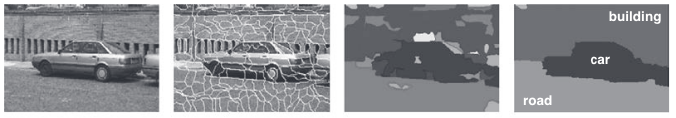
\includegraphics[width=0.9\textwidth]{img/Markov-network-computer-vision.png}
    \caption{Markov Random Fields for Computer Vision: Pairwise connections between adjacent superpixels for compatibility of segmentation labels.}
    \end{figure}
\end{center}
\begin{itemize}
    \item Nodes $\leftrightarrow$ (super-)pixels.
\item Unary factors: compatibility between pixel and class assignment.
\item Pairwise factors: compatibility between neighboring pixels (are they similar $\Rightarrow$ prefer same class assignment of both).
\end{itemize}
\end{example}
\end{frame}


\begin{frame}{Independencies, Soundness, Factorization $\Rightarrow$ I-Map}
\begin{definition}[Separation]
    A set of nodes $Z$ separates $X$ and $Y$ in a Markov network $H = (\mathcal{X},E)$ if there is no path between nodes in $X$ and $Y$ that does not intersect with $Z$.
    We define the global independencies of $H$ as 
    \begin{equation}
        \mathcal{I}(H) = \{(X \indep Y | Z) \mid Z \text{ separates } X \text{ and } Y\}\,.
    \end{equation}
\end{definition}
\pause
\begin{theorem}[Soundness of Separation]
    Let $\Pb$ be a Gibbs distribution that factorizes over $H = (\mathcal{X},E)$, then $H$ is an I-map for $\Pb$.
\end{theorem}
\pause
\begin{proof}
Let $X$, $Y$ and $Z$ be three disjoint subsets such that $Z$ separates $X$ and $Y$.
Assume $X \cup Y \cup Z = \mathcal{X}$.
\pause
As $Z$ separates $X$ and $Y$ there are no direct edges between $X$ and $Y$.
\pause
Hence any clique in $H$ is contained in either $X \cup Z$ or in $Y \cup Z$.
\pause
Let $\mathcal{I}_X$ be the indexes of cliques contained in $X \cup Z$ and $\mathcal{I}_Y$ those in $Y \cup Z$.
\pause
Then 
\begin{equation}
    \Pb[X_1,\ldots,X_n] =
     \frac{1}{Z} \prod_{i \in \mathcal{I}_X} \phi_i\left(X_{\Scope[\phi_i]}\right) \prod_{i \in \mathcal{I}_Y} \phi_i\left(X_{\Scope[\phi_i]}\right) 
     \pause 
     = \frac{f(X,Z)}{\sum_{X} f(X,Z)} \frac{g(Y,Z)}{\sum_{Y} g(Y,Z)}
\end{equation}
\pause
Independence follows from the factorization as a common cause Bayesian network.
\pause
Now consider the case that $U = \mathcal{X} \setminus (X \cup Y \cup Z) \neq \emptyset$.
\pause 
Partition $U$ into $U_1$ and $U_2$ such that $Z$ separates $X \cup U_1$ and $Y \cup U_2$.
\pause 
As above, $X,U_1 \indep Y, U_2 | Z$. 
\pause 
The decomposition property~\eqref{appendix:conditional-independence-properties} implies $X \indep Y | Z$.
\end{proof}
\end{frame}

\begin{frame}{Hammersley Clifford, I-Map $\Rightarrow$ Factorization}
\begin{theorem}[Hammersley Clifford Theorem]
    Let $\Pb$ be a positive distribution and $H = (\mathcal{X},E)$ be a Markov network. If $H$ is an I-map for $\Pb$, then $\Pb$ is a Gibbs distribution that factorizes over $H$.
\end{theorem}
%\pause
%\begin{proof}
%    Will be given later.
%\end{proof}
\pause
\begin{itemize}
    \item Proof will be given later.
\end{itemize}
\pause
\begin{example}[Hammersley Clifford Positivity Condition Necessary]
Let $X_1,\ldots,X_4$ be random binary variables giving probability $1/8$ to
\begin{equation}
\begin{array}{c}
    (0,0,0,0)\quad(1,0,0,0)\quad(1,1,0,0)\quad(1,1,1,0) \\%\quad
    (0,0,0,1)\quad(0,0,1,1)\quad(0,1,1,1)\quad(1,1,1,1)
\end{array}
\end{equation}
and $0$ to all other configurations.
Let $H$ be the graph $X_1 - X_2 - X_3 - X_4 - X_1$.
Then $\Pb$ satisfies independence properties associated with $H$ but $\Pb$ does not factorize according to $H$.
\end{example}
\begin{proof}
\begin{itemize}
    \pause \item Global independencies hold:
Consider $X_1 \indep X_3 | X_2, X_4$.
\pause
For $X_2 = 1, X_4 = 0$ only $X_1 = 1$ will have probability $>0$, thus $\Pb[X_1 = 1 | X_2=1, X_4=0] = 1$ and $X_1$ is trivially independent of $X_3$ given $X_2,X_4$.
\pause
Similar holds true for all other cases, hence global independencies hold.
\pause
\item $\Pb$ does not factorize:
Assume 
$\Pb = \phi_{12}(X_1,X_2) \phi_{23}(X_2,X_3) \phi_{34}(X_3,X_4) \phi_{14}(X_1,X_4)$, i.e. $\Pb$ factorizes according to $H$.
\pause
Since for any state of $X_1,X_2$ there exists states of $X_3,X_4$ that have positive probability, $\phi_{12} > 0$ must hold.
\pause
Similarly $\phi_{23},\phi_{34},\phi_{14} > 0$, which implies $\Pb > 0$.
\end{itemize}
\end{proof}
\end{frame}

\begin{frame}{Completeness of Separation}
\begin{theorem}[Completeness]
Let $H$ be a Markov network structure.
If $X$ and $Y$ are not separated given $Z$ in $H$, then $X$ and $Y$ are dependent given $Z$ in some distribution $\Pb$ that factorizes over $H$.
\end{theorem}
\pause
\begin{proof}
We construct a suitable distribution $\Pb$.
We assume w.l.o.g.\ that all random variables are binary.
\pause
Since $X$ and $Y$ are not separated, there exists a path $X = U_1 - \dots - U_k = Y$ not blocked by $Z$. Choose a minimal length such path.
\pause 
For any $i$ there exists a clique $C_i$ with $U_i, U_{i+1} \in C_i$.
\pause
Define $\phi_{C_i}(X_{\Scope[\phi_{C_i}]}) = \begin{cases} W, & U_i = U_{i+1} \\ 0,& \text{otherwise} \end{cases}$ with $W \gg 0$.
\pause
Note that $C_i \neq C_{i+1}$, since otherwise the path would not be a shortest one.
\pause
All other cliques are uniformly $1$.
\pause
In this distribution $X$ and $Y$ are dependent and the factorization respects $H$.
\end{proof}
\end{frame}

\begin{frame}{Local Independencies}
    \begin{itemize}
    \item Local independencies analoguous to the Bayesian case.
    \item But they are weaker than the global independencies!
    \end{itemize}
    \pause
\begin{definition}[Pairwise Independence]
    Let $H$ be a Markov network.
    We define the pairwise independencies associated with $H$ to be
    \begin{equation}
    \mathcal{I}_p(H) = \{ X \indep Y | \mathcal{X} \backslash \{X,Y\} : \{X,Y\} \notin E)\,.
    \end{equation}
\end{definition}
    \pause
    \begin{definition}[Markov Blanket Independencies]
        For a graph $H$ we define the Markov blanket $\MB_H(X)$ as the neighbors of $X$.
        We define the local independencies associated with $H$ to be
        \begin{equation}
        \mathcal{I}_l(H) = \{X \indep \mathcal{X} \backslash \{X\} - \MB_H(X) | \MB_H(X)\}\,.
        \end{equation}
    \end{definition}
    \begin{itemize}
    \item Trivially $\mathcal{I}_p(H) \subseteq \mathcal{I}_l(H) \subseteq \mathcal{I}(H)$, hence global implies local which in turn implies pairwise independency
    \item Under positivity assumption all three independency definitions are equivalent.
    \end{itemize}
\end{frame}

\begin{frame}{Equivalence of Dependency Definitions}
\begin{theorem}[Pairwise $\Rightarrow$ Global Independency]
Let $\Pb$ be a positive distribution. 
If $\Pb$ satisfies $\mathcal{I}_p(H)$ then it satisfies $\mathcal{I}(H)$.
\end{theorem}
\pause
\begin{proof}
    We want to prove that $X \indep Y | Z$ whenever $Z$ separates $X$ and $Y$.
    We proceed by reverse induction in the size of $Z$.
    \pause
    For $\abs{X} = n-2$ the global independency reduces to the pairwise one.
    \pause 
    Let now $\abs{Z} = k-1$ and let the theorem hold for any $Z'$ with $\abs{Z'} \geq k$.
    \pause
    \begin{itemize}
    \item Case 1: $\abs{X} \geq 2$ or $\abs{Y} \geq 2$. 
    \pause W.l.o.g. $\abs{X} \geq 2$.Choose some $A \in X$.
    It holds that $X \backslash \{A\} \indep Y | Z \cup \{A\}$ due to monotonicity.
    Also $Y$ and $A$ are separated by $Z$, so we have $A \indep Y | Z \cup \mathcal{X} \backslash \{A\}$ by the induction assumption.
    \pause
    Because $\Pb$ is positive, we can apply the intersection property~\eqref{eq:intersection-property} and conclude that
    $X \indep Y | Z$.
    \pause \item Case 2: $\abs{X} = \abs{Y} = 1$.
    \pause
    If $X \cup Y \cup Z = \mathcal{X}$ we refer to the base case.
    \pause Hence there exists an element $A \in \mathcal{X} \backslash (X \cup Y \cup Z)$. 
    \pause If $A$ is not reachable from $Y$ without going over $Z$, by the induction hypothesis it holds that $X \cup \{A\} \indep Y | Z$. By decomposition~\eqref{eq:decomposition-property} we infer $X \indep Y | Z$.
    \pause Analoguously if $A$ is not reachable from $X$.
    \pause The case that $A$ can be reached from both $X$ and $A$ is not possible, since then $Z$ would not separate them.
    \end{itemize}
\end{proof}
\pause
\begin{corollary}
    If $\Pb$ is positive: 
        $\mathcal{I}_p(H)$ is an I-map for $\Pb$
        $\Leftrightarrow$
        $\mathcal{I}_l(H)$ is an I-map for $\Pb$
        $\Leftrightarrow$
        $\mathcal{I}(H)$ is an I-map for $\Pb$.
\end{corollary}
\end{frame}

%\begin{frame}{Log-Linear Models, Energies?}
%\end{frame}


%\begin{frame}{D-Separation $\Leftrightarrow$ Separation in Upward Closure}
%\begin{proof}
%    Let $X$ and $Y$ be separated by $Z$ in the upward closure $G'$.
%    Let $U_1 \Leftrightarrow \ldots \Leftrightarrow U_k$ be a trail in $G$.
%    The trail corresponds to a path in $G'$ after potential shortcutting when using a moral edge.
%\end{proof}
%\end{frame}

\begin{frame}{Energy, Parametrization}
    \begin{definition}[Energy]
    Given a positive Gibbs distribution $\Pb$ with factors $\phi_1,\ldots,\phi_k$ its energy is defined as 
    \begin{equation}
        E(X_1,\ldots,X_n) = \log(\Pb[X_1,\ldots,X_n]) = \sum_{i=1}^k \log(\phi_i(X_{\Scope[\phi_i]}))
    \end{equation}
    We denote energy terms by $\epsilon_i := \log(\phi_i)$.
    \end{definition}
    \pause
\begin{example}[Non-Uniqueness of Parametrizations of Gibbs Distributions]
    \begin{minipage}{0.4\textwidth}
    \begin{center}
    \begin{tikzpicture}
    \node[rand_var] (X1) at (0,3) {$X_1$};
    \node (x11) at (0,0) {$\bullet$};
    \only<5->{\node at (-0.4,0) {\scriptsize$+\delta$};}
    \node (x12) at (0,1) {$\bullet$};
    \node (x13) at (0,2) {$\bullet$};
    \draw (-0.2,-0.2) -- (-0.2,2.2) -- (0.2,2.2) -- (0.2,-0.2) -- cycle;
    \node[rand_var] (X2) at (3,3) {$X_2$};
    \node (x21) at (3,0) {$\bullet$};
    \node (x22) at (3,1) {$\bullet$};
    \node (x23) at (3,2) {$\bullet$};
    \draw (2.8,-0.2) -- (2.8,2.2) -- (3.2,2.2) -- (3.2,-0.2) -- cycle;
    \draw[-] (x11) -- (x21)node[near start, below] {\scriptsize$-\delta$};
    \only<5->{\draw[-] (x11) -- (x21) node[near start, below] {\scriptsize$-\delta$}};
    \draw[-] (x11) -- (x22) node[near start, below] {\scriptsize$-\delta$};
    \only<5->{\draw[-] (x11) -- (x22) node[near start, below] {\scriptsize$-\delta$};}
    \draw[-] (x11) -- (x23) node[near start, below] {\scriptsize$-\delta$};
    \only<5->{\draw[-] (x11) -- (x23) node[near start, below] {\scriptsize$-\delta$};}
    \draw[-] (x12) -- (x21);
    \draw[-] (x12) -- (x22);
    \draw[-] (x12) -- (x23);
    \draw[-] (x13) -- (x21);
    \draw[-] (x13) -- (x22);
    \draw[-] (x13) -- (x23);
    \pause
    \draw[fill=blue!80,nearly transparent, rounded corners]
    (-0.3,-0.3) -- (-0.3,2.3) -- (0.3,2.3) -- (0.3,-0.3) -- cycle;
    \pause
    \draw[fill=green!80,nearly transparent, rounded corners]
    (2.7,-0.3) -- (2.7,2.3) -- (3.3,2.3) -- (3.3,-0.3) -- cycle;
    \pause
    \draw[fill=red!80,nearly transparent, rounded corners]
    (-0.5,-0.5) -- (3.5,-0.5) -- (3.5,2.5) -- (-0.5,2.5) -- cycle;
    \end{tikzpicture}
\end{center}
\end{minipage}
\begin{minipage}{0.59\textwidth}
    Let a Gibbs distribution with $\mathcal{X} = \{X_1,X_2\}$ and factors 
    \begin{itemize}
    \item unary: $\Scope[\textcolor{blue}{\phi_1}] = \{X_1\}$, $\Scope[\textcolor{green}{\phi_2}] = \{X_2\}$,
    \item pairwise: $\Scope[\textcolor{red}{\phi_{12}}] = \{X_1, X_2\}$ 
    \end{itemize}
    be given.
    Let the label space be $L_{X_i} = \{0,1,2\}$.
    Then 
    \begin{itemize}
    \item $\phi_1(x_1) \leftarrow \begin{cases} \phi_1(x_1) + \delta, & x_1 = 0, \\ \phi_{1}(x_1), & \text{otherwise}\end{cases}$
    \item $\phi'_{12}(x_1,x_2) \leftarrow \begin{cases} \phi_{12}(x_1,x_2) - \delta, & x_1 = 0, \\ \phi_{12}(x_1,x_2), & \text{otherwise}\end{cases}$
    \end{itemize}
    produces the same distribution for any $\delta \in \R$.
\end{minipage}
\end{example}
\end{frame}

\begin{frame}{Canonical Parametrization}
    \begin{itemize}
        \item Is there a way to arrive at a unique representative parametrization?
    \end{itemize}
\begin{definition}[Canonical Parametrization]
    Let a positive Gibbs distribution with factors $\phi_1,\ldots,\phi_k$ be given. 
    Fix an arbitrary assignment $\xi^* = (x_1^*, \ldots, x_n^*)$.
    We will refer to factors by specifying their scopes.
    \pause
    For any factor $\phi_i$ add additional factors for any subset $D \subsetneq \Scope[\phi_i]$.
\pause
    The canonical energy function for a clique $D$ is
    \begin{equation}
        \label{eq:canonical-energy-function}
        \epsilon_D(X_D) = \sum_{Z \subseteq D} (-1)^{\abs{D \backslash Z}} \log(\Pb(X_Z, \xi^*_{\mathcal{X} \backslash Z}))\,
    \end{equation}
    where the empty clique $\varnothing$ is also included.
\end{definition}
\begin{itemize}
\pause \item The canonical energy function~\eqref{eq:canonical-energy-function} performs an inclusion/exclusion summation.
\pause \item It is not useful for actual computations, but will help us in the proof of Hammersley Clifford.
\end{itemize}
\pause
\begin{theorem}[Soundness of Canonical Parametrization]
    Let $\Pb$ be a positive Gibbs distribution. The canonical parametrization gives the same probability distribution, i.e.\ 
    \begin{equation}
        \label{eq:canonical-parametrization}
        \Pb[x] = \exp\left(\sum_{i} \epsilon_{i}(x_{\Scope[\epsilon^*_i]})\right)\,.
    \end{equation}
    In particular, its partition function $Z$ is 1.
\end{theorem}
\end{frame}

\begin{frame}{Soundness of Canonical Parametrization, Proof}
\begin{proof}
    First, let $H=(\mathcal{X},E)$ be the complete graph.
\pause
For $Z = \mathcal{X}$ there is exactly one factor $\epsilon_{\mathcal{X}}$ that by construction has one term $\log(\Pb[X_{\mathcal{X}}])$ in $\epsilon_{\mathcal{X}}$.
\pause
For all other $Z \subsetneq \mathcal{X}$ we need to prove $\log(\Pb[X_Z, \xi^*_{\mathcal{X} \backslash Z}])$ appears equally often with negative and positive signs.

\pause 
The term $\log(\Pb[X_Z,\xi^*_{\mathcal{X} \backslash Z}])$ will appear in $\epsilon_D$
\begin{itemize}
\pause \item once, i.e.\ $= \binom{\abs{\mathcal{X}} - \abs{Z}}{0}$ for any $D$ with $\abs{D} = \abs{Z}$ with sign $+1$ (in $\epsilon_Z$),
\pause \item $\abs{\mathcal{X}} - \abs{Z} = \binom{\abs{\mathcal{X}} - \abs{Z}}{1}$ times for any $D$ with $\abs{D} = \abs{Z}+1$ with sign $-1$,
\pause \item $\binom{\abs{\mathcal{X}} - \abs{Z}}{2}$ times for any $D$ with $\abs{D} = \abs{Z}+2$ with sign $+1$,
\pause \item $\ldots$
\end{itemize}
Hence $\log(\Pb[X_Z, \xi^*_{\mathcal{X} \backslash{Z}}])$ appears in sum with coefficient
\begin{equation}
    \sum_{k=0}^{\abs{\mathcal{X}} -\abs{Z}} \binom{\abs{\mathcal{X}} - \abs{Z}}{k} (-1)^k
    \pause = (1 - 1)^{\abs{\mathcal{X}} - \abs{Z}}
    \pause = 0\,
\end{equation}
\pause
The proof for $H$ being not the complete graph will be a by-product of the proof of the Hammersley Clifford theorem.
\end{proof}
\end{frame}

\begin{frame}{Proof of Hammersley Clifford}
\begin{theorem}[Hammersley Clifford Theorem]
    $\Pb$ positive, $H$ a Markov network. $\mathcal{I}(H) \subseteq \mathcal{I}(\Pb)$ $\Rightarrow$ $\Pb$ is a Gibbs distribution that factorizes over $H$.
\end{theorem}
\begin{proof}
    We show existence of a Gibbs parametrization for any distribution $\Pb$ that satisfies the Markov assumption of $H$.
    \pause
    For this, we will construct the Gibbs parametrization using the canonical parametrization.
    \pause
    For any subset $D \subseteq \mathcal{X}$ (also $D$ that are not cliques) define $\epsilon_D$ as in~\eqref{eq:canonical-energy-function}.
    \pause 
    As seen above the resulting Gibbs distribution is $\Pb$.
    \pause
    It remains to show that the distribution factorizes over $H$.
    \pause 
    To this end we show that $\epsilon_D$ are identically zero whenever $D$ is not a clique in $H$.
    \pause 
    Assume we have $X, Y \in D$ such that there is no edge between $X$ and $Y$.
    \pause
    Then for any configuration $d$ of the random variables $\mathcal{X}$
    \begin{equation}
        \epsilon_D(d) = \sum_{Z \subseteq D} (-1)^{\abs{D \backslash Z}} \log(\Pb[d_Z, \xi^*_{\mathcal{X} \backslash Z}])\,.
    \end{equation}
    \pause 
    We rearrange the sum into groups of subsets.
    For $W \subseteq D \backslash \{X,Y\}$ the sets $W$, $W\cup \{X\}$, $W \cup \{Y\}$ and $W \cup \{X,Y\}$ are subsets of $D$.
    \pause
    We can rewrite the above summation as
    \begin{multline}
        \epsilon_D(d) =  \sum_{W \subseteq D \backslash \{X,Y\}} (-1)^{\abs{D \backslash \{X,Y\} \backslash W}} 
        \Big(
        \log(\Pb[d_W, \xi^*_{\mathcal{X} \backslash W}]) 
        - \log(\Pb[d_{W \cup \{X\}}, \xi^*_{\mathcal{X} \backslash (W \cup \{X\})}]) \\
        - \log(\Pb[d_{W \cup \{Y\}}, \xi^*_{\mathcal{X} \backslash (W \cup \{Y\})}])
        + \log(\Pb[d_{W \cup \{X,Y\}}, \xi^*_{\mathcal{X} \backslash (W \cup \{X,Y\})}])
        \Big)
    \end{multline}
\end{proof}
\end{frame}

\begin{frame}{Proof of Hammersley Clifford II}
    \begin{proof}
    Consider a specific $W$ in the above sum. 
    \begin{equation}
    \begin{aligned}
        & \log(\Pb[d_{W \cup \{X,Y\}}, \xi^*_{\mathcal{X} \backslash (W \cup \{X,Y\})}])
        - \log(\Pb[d_{W \cup \{X\}}, \xi^*_{\mathcal{X} \backslash (W \cup \{X\})}])  \\
        \pause = & \log(\frac{\Pb[d_{X}, d_{Y}, d_{W},\xi^*_{\mathcal{X} \backslash D}]}{\Pb[d_{X},\xi^*_{Y},d_{W},\xi^*_{\mathcal{X} \backslash D}]}) \\
        \pause = & \log(\frac{\Pb[d_{Y} | d_{X}, d_{W},\xi^*_{\mathcal{X} \backslash D}] \Pb[d_{X}, d_{W}, \xi^*_{\mathcal{X} \backslash D}]}{ \Pb[\xi^*_{Y} | d_{X}, d_{W},\xi^*_{\mathcal{X} \backslash D}] \Pb[d_{X}, d_{W}, \xi^*_{\mathcal{X} \backslash D}] } \\
        \pause = & \log(\frac{\Pb[d_{Y} | \xi^*_{X}, d_{W},\xi^*_{\mathcal{X} \backslash D}] \Pb[\xi^*_{X}, d_{W}, \xi^*_{\mathcal{X} \backslash D}]}{ \Pb[\xi^*_{Y} | \xi^*_{X}, d_{W},\xi^*_{\mathcal{X} \backslash D}] \Pb[\xi^*_{X}, d_{W}, \xi^*_{\mathcal{X} \backslash D}] } \\
        \pause = & \log(\frac{\Pb[\xi^*_{X}, d_{Y}, d_{W}, \xi^*_{\mathcal{X} \backslash D}]}{\Pb[\xi^*_{X}, \xi^*_{Y},d_{W}, \xi^*_{\mathcal{X} \backslash D}]}) \\
        \pause = &
        \log(\Pb[d_{W \cup \{Y\}}, \xi^*_{\mathcal{X} \backslash (W \cup \{Y\})}])
        - \log(\Pb[d_{W}, \xi^*_{\mathcal{X} \backslash (W)}])  \\
    \end{aligned}
\end{equation}
\pause The third equality is due to $X \indep Y | \mathcal{X} \backslash \{X,Y\}$.
\pause Hence terms sum to zero and the claim follows.
\end{proof}
\end{frame}

\begin{frame}{Bayesian Networks and Markov Networks}
    \begin{itemize}
        \pause \item Can we go from Bayesian networks to Markov ones and back?
    \end{itemize}
    \begin{proposition}[Bayesian $\rightarrow$ Markov]
        Let $G$ be a Bayesian network for $\Pb$. 
        Then $\Pb$ is a Gibbs distribution defined by the factors $\phi_{X_i} = \Pb[X_i | \Pa{G}{X_i}]$.
        The partition function is \pause $1$.
    \end{proposition}
    \begin{proof}
        Immediate from the definitions.
    \end{proof}
    \pause
\begin{itemize}
    \item The proposition above shows that to make a Bayesian network a Markov one edges between parents must be added.
\end{itemize}
    \pause
    \begin{definition}[Moralization]
       The moral graph $\mathcal{M}[G]$ of a Bayesian network structure $G$ is the undirected graph that contains an undirected edge $\{X,Y\}$ whenever $X \rightarrow Y$ or $X \leftarrow Y$ is present in $G$ or $X$ and $Y$ are parents of the same node.
    \end{definition}
    \begin{itemize}
        \pause \item In other words, the moral graph of a Bayesian network is an I-map for $\Pb$, i.e. $\mathcal{I}(\mathcal{M}(G)) \subseteq \mathcal{I}(\Pb)$.
        \pause \item Unpopular opinion: You \underline{must} marry if you have children!
        \pause \item Today's opinion: Moralization might lead to loss of independency.
        \begin{itemize} \item consider independence information of v-structure $X \rightarrow Z \leftarrow Y$). \end{itemize}
    \end{itemize}
\end{frame}

\begin{frame}{Soundness of D-Separation, Proof}
    \begin{itemize}
    \item D-separation soundness cannot be proved by naively looking at the moralized graph:
    \begin{itemize} 
        \pause \item For $X \rightarrow Z \leftarrow Y$ the active trail criterion gives that $X \indep Y$.
        \pause \item  I-map on the moralized graph does not reveal this!
    \end{itemize}
    \pause \item Idea: Remove all unobserved nodes in nodes in v-structures (i.e.\ barren nodes).
    \end{itemize}
    \pause
    \begin{proposition}[D-Separation $\Leftrightarrow$ Separation in Upward Closure]
    Let $X, Z, Y$ be three sets of nodes in a Bayesian network $G$.
    Let $U = X \cup Y \cup Z$ and let the upward closure be $G' = \Mor[G[U \cup \Anc[U]]$, i.e.\ take the induced graph of $U \cup \Anc[U]$ and moralize it.
    Then $X$ and $Y$ are d-separated in $G$ if and only if they are separated in $G'$.
    \end{proposition}
    \pause
    \begin{example}[Upward Closure]
    \begin{minipage}[t]{0.3\textwidth}
        \centering
        Bayesian network $G$ \\ \vspace{0.1cm}
            \begin{tikzpicture}[baseline=(I.base), scale=0.6]
                \node [rand_var] (I) at (0, 5) {I};
                \node [rand_var] (G) at (-1, 4) {G};
                \node [rand_var] (D) at (-2, 5) {D};
                \node [rand_var] (L) at (-1, 3) {L};
                \node [rand_var] (J) at (0, 2) {J};
                \node [rand_var] (A) at (0, 3) {A};
                \node [rand_var] (S) at (1, 4) {S};
                \draw[->] (D) to (G);
                \draw[->] (I) to (G);
                \draw[->] (G) to (L);
                \draw[->] (L) to (J);
                \draw[->] (A) to (J);
                \draw[->] (I) to (S);
                \draw[->] (S) to (J);
        \end{tikzpicture}
    \end{minipage} 
    \pause
    \hfill \vrule \hfill
    \begin{minipage}[t]{0.32\textwidth}
        \centering
        $\Mor[\{D,I,L\} \cup \Anc[\{D,I,L\}]]$ \\ \vspace{0.1cm}
        \begin{tikzpicture}[baseline=(I.base), scale=0.6]
                \node [rand_var] (I) at (0, 5) {I};
                \node [rand_var] (G) at (-1, 4) {G};
                \node [rand_var] (D) at (-2, 5) {D};
                \node [rand_var] (L) at (-1, 3) {L};
                \node [rand_var, gray!30] (J) at (0, 2) {J};
                \node [rand_var, gray!30] (A) at (0, 3) {A};
                \node [rand_var, gray!30] (S) at (1, 4) {S};
                \draw (D) to (G);
                \draw (I) to (G);
                \draw (G) to (L);
                \draw (D) to (I);
                \draw[gray!30] (L) to (J);
                \draw[gray!30] (A) to (J);
                \draw[gray!30] (I) to (S);
                \draw[gray!30] (S) to (J);
       \end{tikzpicture}
    \end{minipage}
    \pause
        \hfill \vrule \hfill
    \begin{minipage}[t]{0.36\textwidth}
        \centering
        $\Mor[\{D,I,A,S\} \cup \Anc[\{D,I,A,S\}]]$ \\ \vspace{0.1cm}
        \begin{tikzpicture}[baseline=(I.base), scale=0.6]
                \node [rand_var] (I) at (0, 5) {I};
                \node [rand_var, gray!30] (G) at (-1, 4) {G};
                \node [rand_var] (D) at (-2, 5) {D};
                \node [rand_var, gray!30] (L) at (-1, 3) {L};
                \node [rand_var, gray!30] (J) at (0, 2) {J};
                \node [rand_var] (A) at (0, 3) {A};
                \node [rand_var] (S) at (1, 4) {S};
                \draw[gray!30] (D) to (G);
                \draw[gray!30] (I) to (G);
                \draw[gray!30] (G) to (L);
                \draw[gray!30] (D) to (I);
                \draw[gray!30] (L) to (J);
                \draw[gray!30] (A) to (J);
                \draw (I) to (S);
                \draw[gray!30] (S) to (J);
        \end{tikzpicture}
    \end{minipage}
    \end{example}
    \pause
    \begin{proof}
        Path from $X$ to $Y$ in $G'$
        \pause $\Leftrightarrow$ Path can shortcut any v-structure
        \pause $\Leftrightarrow$ $\exists$ active trail in $G$.
    \end{proof}
\end{frame}

\begin{frame}{D-Separation, Proof}
    \begin{itemize}
        \item Recall that we did not yet prove that d-separation is sound, see slide~\ref{slide:d-separation}.
        \pause
        \item We can return to the Markov case through the upward closure and use it to derive d-separation soundness.
    \end{itemize}
    \pause 
    \begin{theorem}[Soundness of d-separation]
    If a distribution $\Pb$ factorizes according to $G$, then $\mathcal{I}(G) \subseteq \mathcal{I}(\Pb)$.
    \end{theorem}
    \begin{proof}
        Let $U = X \cup Y \cup Z$, let $U^* = U \cup \Anc[U]$, let $G_{U^*}$ be the induced graph over $U^*$ and let $H$ be the moralized graph of $G_{U^*}$.
        \pause
        Let $\Pb_{U^*}$ be the Bayesian network distribution defined over $G_{U^*}$.
        \pause
        Consider an independence assertion $X \indep Y | Z \in \mathcal{I}(G)$.
        We want to prove that this holds for $\Pb$.
        \pause
        By definition we have that $X$ and $Y$ are d-separated given $Z$ in $G$.
        This is equivalent to $X$ and $Y$ begin separated in $H$ given $Z$, and hence $X \indep Y | Z$.
        \pause 
        Since $P_{U^*}[X_{U^*}] =\Pb[X_{U^*}]$ (see Lemma \ref{lemma:Bayesian-network-restriction}), this is equivalent to $X \indep Y | Z$ in $\Pb$.
    \end{proof}
\end{frame}

\begin{frame}{Factor Graph}
\begin{columns}
    \column{0.35\textwidth}
    \begin{itemize}
        \item What can we say about factors of a Gibbs distribution $\Pb$ that factorize according to
    \end{itemize}
    \column{0.1\textwidth}
    \begin{tikzpicture}[baseline=(3.base)]
        \node[rand_var] (1) at (0,0) {$1$};
        \node[rand_var] (2) at (1,0) {$2$};
        \node[rand_var] (3) at (0,-1) {$3$};
        \node[rand_var] (4) at (1,-1) {$4$};
        \draw (1) -- (2);
        \draw (1) -- (3);
        \draw (1) -- (4);
        \draw (2) -- (4);
        \draw (3) -- (4);
    \end{tikzpicture}
    \column{0.55\textwidth}
    \begin{itemize}
        \pause \item $\Pb_c[X_{1:4}] = \frac{1}{Z} \phi_{124}(X_1,X_2,X_4) \phi_{134}(X_1,X_3,X_4)$.
        \pause \item $\Pb_p[X_{1:4}] = \frac{1}{Z} \phi_{12}(X_1,X_2)\allowbreak \phi_{13}(X_1,X_3)\allowbreak \phi_{14}(X_1,X_4)\allowbreak \phi_{24}(X_2,X_4)\allowbreak \phi_{34}(X_3,X_4)$
        \pause \item Or something in between?
    \end{itemize}
\end{columns}
\pause
\hrule
\begin{itemize}
    \item Graph structure does not reveal factorization structure uniquely.
    \pause\item We need a finer structure for this: The Factor Graph.
\end{itemize}
\pause
\hrule
\begin{definition}[Factor Graph]
    Giben a Gibbs distribution $\Pb$, its factor graph $F$ is an undirected graph whose nodes are the variables and factors of $\Pb$, called \emph{variable nodes} and \emph{factor nodes} respectively.
    Edges in the factor graph are between variables $X$ and factors $\phi$ such that $X \in \Scope[\phi]$.

    We also say that $\Pb$ factorizes over $F$ in this case.
\end{definition}
\pause
\begin{columns}
\column{0.5\textwidth}
\begin{center}
    $\Pb_c$ factorizes over \\ \vspace{0.1cm}
\begin{tikzpicture}
\node[rand_var] (1) at (0,0) {$1$};
\node[rand_var] (2) at (1,0) {$2$};
\node[rand_var] (3) at (2,0) {$3$};
\node[rand_var] (4) at (3,0) {$4$};
\node[factor_var] (124) at (0.5,1.5) {$\phi_{124}$};
\node[factor_var] (134) at (2.5,1.5) {$\phi_{134}$};
\draw (1) -- (124);
\draw (2) -- (124);
\draw (4) -- (124);
\draw (1) -- (134);
\draw (3) -- (134);
\draw (4) -- (134);
\end{tikzpicture}
\end{center}
\pause
%\hfill \vrule \hfill
\column{0.5\textwidth}
\begin{center}
    $\Pb_p$ factorizes over \\ \vspace{0.1cm}
\begin{tikzpicture}
\node[rand_var] (1) at (0,0) {$1$};
\node[rand_var] (2) at (1,0) {$2$};
\node[rand_var] (3) at (2,0) {$3$};
\node[rand_var] (4) at (3,0) {$4$};
\node[factor_var] (12) at (-0.5,1.5) {$\phi_{12}$};
\node[factor_var] (13) at (0.5,1.5) {$\phi_{13}$};
\node[factor_var] (14) at (1.5,1.5) {$\phi_{14}$};
\node[factor_var] (24) at (2.5,1.5) {$\phi_{24}$};
\node[factor_var] (34) at (3.5,1.5) {$\phi_{34}$};
\draw (1) -- (12);
\draw (1) -- (13);
\draw (1) -- (14);
\draw (2) -- (12);
\draw (2) -- (24);
\draw (3) -- (13);
\draw (3) -- (34);
\draw (4) -- (14);
\draw (4) -- (24);
\draw (4) -- (34);
\end{tikzpicture}
\end{center}
\end{columns}
\end{frame}

\section{Inference}

\begin{frame}{Inference: Questions}
\begin{itemize}
\item How to compute marginal probabilities $\Pb[X]$ for some variables $X \subseteq \mathcal{X}$?
\begin{itemize}
    \pause \item given evidence $\Pb[X | Y = e]$?
\end{itemize}
\pause \item How to draw samples $x \sim \Pb[X]$ given a probability distribution?
\begin{itemize}
    \pause \item given evidence $x \sim \Pb[X | Y = e]$?
\end{itemize}
\pause \item How to find most probable assignment $\argmax_{x} \Pb[x]$ (resp.\ conditional version)?
\pause \item In Markov networks: How to compute the partition function $Z$?
\pause \item Naive approach for marginal probabilities: Consider all possible assignments? 
\begin{itemize}
\pause \item Compute $\Pb[x,e] = \sum_{w} \Pb[x,e,w]$ where $w$ all non-observed variables we are not interested in.
\pause \item Next compute $\Pb[e] = \sum_{x} \Pb[x,e]$,
%\pause \item Draw samples according to $\Pb[X | Y = e] = \frac{\Pb[X,e]}{\Pb[e]}$, examining each.
\pause \item Not scalable, exponential blowup!
\pause \item In general inference is NP-hard: better general methods not probable to exist.
\pause \item Still worth studying: 
\begin{itemize}
    \item Fast exact methods possible in special cases.
    \pause \item Approximate methods might be good enough in practice.
\end{itemize}
\end{itemize}
\pause \item Can we exploit network structure if $\Pb$ is a $\{$Bayesian$|$Markov$\}$ network?
\end{itemize}
\end{frame}

%\subsection{Exact Inference with Variable Elimination}

\begin{frame}{Variable Elimination: Intuition}
    \begin{example}[Chain Graph BN]
    \begin{tikzpicture}[baseline={(A.base)}]
    \node[rand_var] (A) at (0,0) {$A$};
    \node[rand_var] (B) at (1,0) {$B$};
    \node[rand_var] (C) at (2,0) {$C$};
    \node[rand_var] (D) at (3,0) {$D$};
    \draw[->] (A) -- (B);
    \draw[->] (B) -- (C);
    \draw[->] (C) -- (D);
    \end{tikzpicture}

    \begin{itemize}
        \pause \item Factorization $\Pb[A,B,C,D] = \Pb[A] \Pb[B | A] \Pb[C | B] \Pb[D | C]$.
    \pause \item Goal: Compute $\Pb[B] \pause = \sum_a \Pb[a] \Pb[B | a]$. \pause All needed factors present in BN.
    \pause \item Goal: Compute $\Pb[C] \pause = \sum_b \Pb[b] \Pb[C | b]$. 
    \pause \item Goal: Compute $\Pb[D] \pause = \sum_c \Pb[c] \Pb[D | c]$. 
    \begin{itemize}
    \pause \item Complexity: $\mathcal{O}(k^2)$, where $k$ is number of states.
    \end{itemize}
    \pause \item General length $n$ chain complexity is \pause $\mathcal{O}(n k^2)$.
    \end{itemize}
    \end{example}
\pause
    \begin{example}[Full Graph BN]
    \begin{tikzpicture}[baseline={(A.base)}]
    \node[rand_var] (A) at (0,0) {$A$};
    \node[rand_var] (B) at (1,0) {$B$};
    \node[rand_var] (C) at (2,0) {$C$};
    \node[rand_var] (D) at (3,0) {$D$};
    \draw[->] (A) -- (B);
    \draw[->] (B) -- (C);
    \draw[->] (C) -- (D);
    \draw[->, bend left=30] (A) to (C);
    \draw[->, bend left=40] (A) to (D);
    \draw[->, bend left=30] (B) to (D);
    \end{tikzpicture}
    \begin{itemize}
        \pause \item Factorization $\Pb[A,B,C,D] = \Pb[A] \Pb[B | A] \Pb[C | A, B] \Pb[D | A,B,C]$.
        \pause \item Compute $\Pb[B]$ as above, $\Pb[C] = \sum_{a,b} \Pb[C | a,b] \Pb[b | a] \Pb[a]$.
        \pause \item $\Pb[D] = \sum_{a,b,c} \Pb[D | a,b,c] \Pb[c | a, b] \Pb[b | a] \Pb[a]$.
        \pause \item We cannot reuse computations as for chain graph.
    \pause \item Complexity using chain rule is \pause $\mathcal{O}(k^n)$!
    \end{itemize}
\end{example}
\end{frame}

\begin{frame}{Variable Elimination}
    \begin{itemize}
        \item Computing $\Pb[X]$ from $\Pb[X,Y]$ requires summing out all $Y$.
    \pause \item To this end: Define a basic operation summation operation on factors
%    \begin{itemize}
%    \item Given a factor $\phi(X,Y)$ (either in Bayesian or Markov network), obtain a marginal factor by summing out all $Y$.
%    \end{itemize}
    \end{itemize}
    \pause
    \begin{definition}[Factor Marginalization]
        Let $X$ be a set of random variables, $Y \notin X$.
        Let $\phi(X,Y)$ be a factor.
        We define the factor marginalization of $Y$ in $\phi$ as 
        \begin{equation}
            \psi(X) = \sum_Y \phi(X,Y)\,.
        \end{equation}
        We call this operation summing out $Y$.
    \end{definition}
    \pause
\begin{itemize}
    \item Idea for summing out variables in probability distribution: Do it one by one.
\end{itemize}
    \pause
    \begin{algorithm}[H]
        \caption{Sum-Product Variable Elimination}
        \vspace{-0.1cm}
        \KwInput{
            Factors $\Phi$,
            variable order $\prec$,
            variables to be eliminated $Z = \{Z_1 \prec \ldots \prec Z_k\}$.
            }
            \For{$i=1,\ldots,k$}{
                \begin{tcolorbox}[boxsep=0pt,width=5cm]
                $\Phi' \leftarrow \{ \phi \in \Phi: Z_i \in \Scope[\phi]\}$\;
                $\Phi'' \leftarrow \Phi \backslash \Phi'$\;
                $\psi \leftarrow \prod_{\phi \in \Phi'} \phi$\;
                $\tau \leftarrow \sum_{Z_i} \psi$\;
                $\Phi \leftarrow \Phi'' \cup \{\tau\}$\;
                \end{tcolorbox}
            }
            \KwOutput{$\Phi$}
        \label{alg:sum-product-variable-elimination}
    \end{algorithm}
\end{frame}

\begin{frame}{Sum-Product Application to Chain Graph}
    \begin{example}[Sum-Product on Chain Graph]
        Recall that the chain graph factorizes as
    \begin{equation}
    \Pb[A,B,C,D] = \phi_A \phi_{AB} \phi_{BC} \phi_{CD}
    \end{equation}
    \pause 
    Then application of Algorithm~\ref{alg:sum-product-variable-elimination} with $Z = \{A \prec B \prec C\}$ gives
    \begin{equation}
        \begin{aligned}
        \pause \Pb[D] = & \sum_{C} \sum_{B} \sum_{A} \phi_A \phi_{AB} \phi_{BC} \phi_{CD} \\
        \pause = & \sum_C \sum_B \phi_{CD} \phi_{BC} \underbrace{\left( \sum_A \phi_A \phi_{AB}\right)}_{= \tau_1, \text{Iteration } 1} \\
        \pause = & \underbrace{\sum_C \phi_{CD} \underbrace{\left(\sum_B \phi_{BC} \left( \sum_A \phi_A \phi_{AB}\right)\right)}_{= \tau_2, \text{Iteration } 2}}_{= \tau_3, \text{Iteration } 3} \\
        \end{aligned}
    \end{equation}
    \end{example}

    \pause
    \begin{itemize}
    \item Efficiency of Sum-Product relies on the fact that
    \begin{equation}
        \sum_X (\phi_1 \phi_2) = \phi_1 \sum_X \phi_2 \quad\quad \text{whenever } X \notin \Scope[\phi_1]\,.
    \end{equation}
    \end{itemize}
\end{frame}

\begin{frame}{Sum-Product Variable Elimination Correctness}
\begin{theorem}[Correctness of Algorithm~\ref{alg:sum-product-variable-elimination}]
Let $X$ be a set of random variables, $\Phi$ a set of factors with $\Scope[\phi] \subseteq X$ for $\phi \in \Phi$.
Let $Y \subseteq X$ be a set of query variables. For any ordering $\prec$ of $X \backslash Y$ Algorithm~\ref{alg:sum-product-variable-elimination}$(\Phi, X \backslash Y, \prec)$ returns a factor $\phi^*(Y)$ such that
\begin{equation}
    \phi^*(Y) = \sum_{X \backslash Y} \prod_{\phi \in \Phi} \phi\,.
\end{equation}
\end{theorem}
\pause
\begin{proof}
Immediate from the observation that Algorithm~\ref{alg:sum-product-variable-elimination} is just a reordering of summations.
\end{proof}
\begin{description}
    \pause \item[Bayesian Network:] Algorithm~\ref{alg:sum-product-variable-elimination} directly gives marginal probabilities:
\begin{equation}
    VE(\Phi, \prec, Z) = \prod_{X_i \notin Z} \Pb[X_i | \Pa{G}{X_i} \backslash Z]\,.
\end{equation}
    \pause \item[Markov Network:] Algorithm~\ref{alg:sum-product-variable-elimination} gives an unnormalized factor over the query. 
    \begin{equation}
    VE(\Phi, \prec, Z) = \sum_{X \in Z} \prod_{i} \phi_i 
    \end{equation}
    \begin{itemize}
        \pause \item Compute partition function to obtain a probability distribution via
        $Z = VE(\Phi, \prec, \mathcal{X})$.
    \end{itemize}
    \pause \item[Evidence:] Given evidence $E = e$ replace factors by $\phi[E = e]$ and apply Algorithm~\ref{alg:sum-product-variable-elimination}.
\end{description}
\end{frame}

\begin{frame}{Variable Elimination: Graph Transformation}
\begin{itemize}
    \item What happens to the factorization during Algorithm~\ref{alg:sum-product-variable-elimination}?
    \pause
    \begin{itemize}
        \item \underline{Graph viewpoint:} When Bayesian, moralize the graph.
    \end{itemize}
    \pause
    \item When a variable is eliminated in Algorithm~\ref{alg:sum-product-variable-elimination}:
    \begin{itemize}
    \pause \item Create factor $\psi$ with $\Scope[\psi] = \{X\} \cup \{Y : \{X,Y\} \in E\}$.
        \begin{itemize}
    \pause \item \underline{Graph viewpoint:} Add all edges in $\Scope[\psi]$ (called fill edges).
        \end{itemize}
    \pause \item Sum out $X$ from $\psi$, obtain factor $\tau$ with $\Scope[\tau] = \Scope[\psi] \backslash \{X\}$.
        \begin{itemize}
    \pause \item \underline{Graph viewpoint:} Remove node $X$ and all adjacent edges.
        \end{itemize}
    \end{itemize}
\end{itemize}
\pause
\hrule
\begin{center}
\begin{tikzpicture}[scale=0.6]
    \node at (0.5,6) {Original graph};
    \node[rand_var] (C) at (-1, 5) {C};
    \node[rand_var] (D) at (-1, 4) {D};
    \node[rand_var] (G) at (0, 3) {G};
    \node[rand_var] (I) at (1, 4) {I};
    \node[rand_var] (L) at (0, 2) {L};
    \node[rand_var] (H) at (-1, 1) {H};
    \node[rand_var] (S) at (1, 1) {S};
    \node[rand_var] (J) at (2, 3) {J};
    \draw[->] (C) to (D);
    \draw[->] (D) to (G);
    \draw[->] (I) to (G);
    \draw[->] (I) to (J);
    \draw[->] (J) to (S);
    \draw[->] (G) to (L);
    \draw[->] (L) to (S);
    \draw[->] (S) to (H);
    \draw[bend right=15,->] (G) to (H);
\pause
    \begin{scope}[shift={(4,0)}]
    \node at (0.5,6) {Moral graph};
    \node[rand_var] (C) at (-1, 5) {C};
    \node[rand_var] (D) at (-1, 4) {D};
    \node[rand_var] (G) at (0, 3) {G};
    \node[rand_var] (I) at (1, 4) {I};
    \node[rand_var] (L) at (0, 2) {L};
    \node[rand_var] (H) at (-1, 1) {H};
    \node[rand_var] (S) at (1, 1) {S};
    \node[rand_var] (J) at (2, 3) {J};
    \draw (C) to (D);
    \draw (D) to (G);
    \draw[blue] (D) to (I);
    \draw (I) to (G);
    \draw (I) to (J);
    \draw (J) to (S);
    \draw (G) to (L);
    \draw[blue, bend left=15] (G) to (S);
    \draw (L) to (S);
    \draw[blue] (L) to (J);
    \draw (S) to (H);
    \draw[bend right=15] (G) to (H);
    \node at (0.5,-0.5) {\textcolor{blue}{$-$}: Moral edge};
    \end{scope}
\pause
    \begin{scope}[shift={(8,0)}]
    \node at (0.5,6) {Eliminate C};
    \node[gray!30, rand_var] (C) at (-1, 5) {C};
    \node[rand_var] (D) at (-1, 4) {D};
    \node[rand_var] (G) at (0, 3) {G};
    \node[rand_var] (I) at (1, 4) {I};
    \node[rand_var] (L) at (0, 2) {L};
    \node[rand_var] (H) at (-1, 1) {H};
    \node[rand_var] (S) at (1, 1) {S};
    \node[rand_var] (J) at (2, 3) {J};
    \draw[gray!30] (C) to (D);
    \draw (D) to (G);
    \draw[blue] (D) to (I);
    \draw (I) to (G);
    \draw (I) to (J);
    \draw (J) to (S);
    \draw (G) to (L);
    \draw[blue, bend left=15] (G) to (S);
    \draw (L) to (S);
    \draw[blue] (L) to (J);
    \draw (S) to (H);
    \draw[bend right=15] (G) to (H);
    \end{scope}
\pause
    \begin{scope}[shift={(12,0)}]
    \node at (0.5,6) {Eliminate D};
    \node[gray!30, rand_var] (C) at (-1, 5) {C};
    \node[gray!30, rand_var] (D) at (-1, 4) {D};
    \node[rand_var] (G) at (0, 3) {G};
    \node[rand_var] (I) at (1, 4) {I};
    \node[rand_var] (L) at (0, 2) {L};
    \node[rand_var] (H) at (-1, 1) {H};
    \node[rand_var] (S) at (1, 1) {S};
    \node[rand_var] (J) at (2, 3) {J};
    \draw[gray!30] (C) to (D);
    \draw[gray!30] (D) to (G);
    \draw[gray!30] (D) to (I);
    \draw (I) to (G);
    \draw[blue] (I) to (J);
    \draw (J) to (S);
    \draw (G) to (L);
    \draw[blue, bend left=15] (G) to (S);
    \draw (L) to (S);
    \draw[blue] (L) to (J);
    \draw (S) to (H);
    \draw[bend right=15] (G) to (H);
    \end{scope}
\pause
    \begin{scope}[shift={(16,0)}]
    \node at (0.5,6) {Eliminate I};
    \node[gray!30, rand_var] (C) at (-1, 5) {C};
    \node[gray!30, rand_var] (D) at (-1, 4) {D};
    \node[rand_var] (G) at (0, 3) {G};
    \node[gray!30, rand_var] (I) at (1, 4) {I};
    \node[rand_var] (L) at (0, 2) {L};
    \node[rand_var] (H) at (-1, 1) {H};
    \node[rand_var] (S) at (1, 1) {S};
    \node[rand_var] (J) at (2, 3) {J};
    \draw[gray!30] (C) to (D);
    \draw[gray!30] (D) to (G);
    \draw[gray!30] (D) to (I);
    \draw[gray!30] (I) to (G);
    \draw[gray!30] (I) to (J);
    \draw[red] (G) to (J);
    \draw (J) to (S);
    \draw (G) to (L);
    \draw[blue, bend left=15] (G) to (S);
    \draw (L) to (S);
    \draw[blue] (L) to (J);
    \draw (S) to (H);
    \draw[bend right=15] (G) to (H);
    \node at (0.5,-0.5) {\textcolor{red}{$-$}: Fill edge};
    \end{scope}
\end{tikzpicture}
\end{center}
\end{frame}

\begin{frame}{Variable Elimination: Induced Graph}
    \label{slide:induced-graph}
\begin{definition}[Induced Graph]
    Let $\Phi$ be a set of factors over $\mathcal{X}$ and $\prec$ be an elimination order.
    The induced graph $\mathcal{I}_{\Phi,\prec}$ is an undirected graph over $\mathcal{X}$ with $X_i - X_j$ if they appear in some intermediate factor $\psi$ generated by Algorithm~\ref{alg:sum-product-variable-elimination} using $\prec$ as elimination order.
\end{definition}
\pause
\begin{itemize}
    \item Elimination order: C $\prec$ D $\prec$ I $\prec$ H $\prec$ G $\prec$ S $\prec$ L.
\end{itemize}
\vspace{-0.4cm}
    \begin{minipage}[t]{0.29\textwidth}
\begin{example}
    \begin{center}
Ind.\ Graph $\mathcal{I}_{\Phi,\prec}$
\begin{tikzpicture}[scale=0.7,baseline={(C.base)}]
    \node[rand_var] (C) at (-1, 5) {C};
    \node[rand_var] (D) at (-1, 4) {D};
    \node[rand_var] (G) at (0, 3) {G};
    \node[rand_var] (I) at (1, 4) {I};
    \node[rand_var] (L) at (0, 2) {L};
    \node[rand_var] (H) at (-1, 1) {H};
    \node[rand_var] (S) at (1, 1) {S};
    \node[rand_var] (J) at (2, 3) {J};
    \draw (C) to (D);
    \draw(D) to (G);
    \draw[blue]  (D) to (I);
    \draw (I) to (G);
    \draw (I) to (J);
    \draw[red] (G) to (J);
    \draw (J) to (S);
    \draw (G) to (L);
    \draw[blue, bend left=15] (G) to (S);
    \draw (L) to (S);
    \draw[blue] (L) to (J);
    \draw (S) to (H);
    \draw[bend right=15] (G) to (H);
\end{tikzpicture}
\end{center}
\end{example}
\end{minipage}
\pause
\begin{minipage}[t]{0.29\textwidth}
\begin{example}
\begin{center}
Cliques of $\mathcal{I}_{\Phi,\prec}$
\begin{tikzpicture}[scale=0.7,baseline={(C.base)}]
    \node[rand_var] (C) at (-1, 5) {C};
    \node[rand_var] (D) at (-1, 4) {D};
    \node[rand_var] (G) at (0, 3) {G};
    \node[rand_var] (I) at (1, 4) {I};
    \node[rand_var] (L) at (0, 2) {L};
    \node[rand_var] (H) at (-1, 1) {H};
    \node[rand_var] (S) at (1, 1) {S};
    \node[rand_var] (J) at (2, 3) {J};
    \draw (C) to (D);
    \draw (D) to (G);
    \draw (D) to (I);
    \draw (I) to (G);
    \draw (I) to (J);
    \draw (G) to (J);
    \draw (J) to (S);
    \draw (G) to (L);
    \draw[bend left=15] (G) to (S);
    \draw (L) to (S);
    \draw (L) to (J);
    \draw (S) to (H);
    \draw[bend right=15] (G) to (H);
    \pause 
    \filldraw[fill=blue!70, nearly transparent, tension=0.7] plot[smooth cycle] coordinates {(C.north west) (D.south west) (D.south east) (C.north east)};
    \pause 
    \filldraw[fill=green!70, nearly transparent, tension=0.7] plot[smooth cycle] coordinates {(D.north west) (G.south) (I.north east)};
    \pause 
    \filldraw[fill=orange!70, nearly transparent, tension=0.7] plot[smooth cycle] coordinates {(I.north) (G.south west) (J.south east)};
    \pause 
    \filldraw[fill=red!50, nearly transparent, tension=0.7, even odd rule] plot[smooth cycle] coordinates {(H.south west) (S.east) (G.north)} (L) circle (0.55cm);
    \pause 
    \filldraw[fill=brown!50, nearly transparent, tension=0.7] plot[smooth cycle] coordinates {(G.north west) (L.south west) (S.south) (J.east) };
    \pause 
    \filldraw[fill=gray!70, nearly transparent, tension=0.7] plot[smooth cycle] coordinates {(S.south) (L.west) (J.north east)};
    \pause 
    \filldraw[fill=black!70, nearly transparent, tension=0.7] plot[smooth cycle] coordinates {(L.south) (J.south) (J.north) (L.north)};
\end{tikzpicture}
\end{center}
\end{example}
\end{minipage}
\pause
\begin{minipage}[t]{0.39\textwidth}
\begin{theorem}
Let $\mathcal{I}_{\Phi,\prec}$ be the induced graph, then:
\begin{itemize}
    \item $\Scope[\psi]$ of every factor $\psi$ generated during Algorithm~\ref{alg:sum-product-variable-elimination} is a clique in $\mathcal{I}_{\Phi,\prec}$.
    \item Every maximal clique in $\mathcal{I}_{\Phi,\prec}$ is the scope of an intermediate factor $\psi$ in the computation.
\end{itemize}
\end{theorem}
\pause
\vspace{-0.35cm}
\begin{proof}
First statement clear from construction.
\pause
For the second, consider the first time $X$ is visited in the maximal clique $C$ creating $\psi$.
\pause
Since $X$ is connected to any other node in the clique, $\Scope[\psi] = C$.
\end{proof}
\end{minipage}
%\textbf{(Maximal) Clique tree:}
%\begin{tikzpicture}[baseline={(CD.base)}]
%    \node[rand_var] (CD) at (0,0) {CD};
%    \node[rand_var] (GID) at (2,0) {GID};
%    \node[rand_var] (GIS) at (4,0) {GIS};
%    \node[rand_var] (GJSL) at (6,0) {GJSL};
%    \node[rand_var] (GHJ) at (8,0) {GHJ};
%    %
%    \draw (CD) to node[below] {D} (GID);
%    \draw (GID) to node[below] {G,I} (GIS);
%    \draw (GIS) to node[below] {G,S} (GJSL);
%    \draw (GJSL) to node[below] {G,J} (GHJ);
%\end{tikzpicture}
\end{frame}

\begin{frame}{Induced Width, Tree Width}
    \begin{definition}[Induced Width]
        The induced width of a graph is the maximal number of variables in a clique minus one.
        The induced width $w_{H,\prec}$ of an order $\prec$ and graph $H$ is the induced width of $\mathcal{I}_{H,\prec}$.
    \end{definition}
    \pause
    \begin{definition}[Tree Width]
       The tree width of a graph $H$ is the minimal induced width over all possible elimination orders $w^*_H = \min_{\prec} \{ w_{H,\prec} \}$.
    \end{definition}
    \pause
    \begin{remark}[Complexity of Algorithm~\ref{alg:sum-product-variable-elimination}]
        The complexity of variable elimination is determined by the induced width as $\mathcal{O}(\abs{\mathcal{X}} \cdot (w_{H,\prec} + 1)^L)$, where $L$ is the maximal number of states of variables in $\mathcal{X}$.
    \end{remark}
    \pause
    \begin{remark}[Finding Best Elimination Order]
        Finding the best elimination order will allow to run Algorithm~\ref{alg:sum-product-variable-elimination} with minimal complexity.
        However, finding the best elimination order is NP-hard.
    \end{remark}
\end{frame}

 \begin{frame}{Naive Bayes Model: Tree Width}
     \begin{example}[Naive Bayes Model]
         \begin{minipage}[t]{0.32\textwidth}
 \begin{center}
 Original Bayesian network
 \\ \  \\
 \begin{tikzpicture}[scale=0.8]
 \node[rand_var] (A) at (0,0) {A};
 \foreach \a in {1,2,...,5}{
     \node[rand_var] (\a) at (-3 + \a, -2) {\a};
     \draw[->] (A) to (\a);
 }
 \end{tikzpicture}
 \end{center}
 \end{minipage}
 \pause
 \begin{minipage}[t]{0.32\textwidth}
     \begin{center}
     Elimination order $A \prec 1 \ldots \prec 5$
 \begin{tikzpicture}[scale=0.8]
\node[rand_var] (A) at (0,0) {A};
\node[rand_var] (1) at (-3 + 1, -2) {1};
\node[rand_var] (2) at (-3 + 2, -2) {2};
\node[rand_var] (3) at (-3 + 3, -2) {3};
\node[rand_var] (4) at (-3 + 4, -2) {4};
\node[rand_var] (5) at (-3 + 5, -2) {5};


\draw (1) to (A);
\draw (2) to (A);
\draw (3) to (A);
\draw (4) to (A);
\draw (5) to (A);

\pause
 \draw[red] (1) to (2);
 \draw[red, bend left=40] (1) to (3);
 \draw[red, bend left=45] (1) to (4);
 \draw[red, bend left=50] (1) to node (15) {} (5);
 \draw[red] (2) to (3);
 \draw[red, bend left=40] (2) to (4);
 \draw[red, bend left=45] (2) to node (25) {} (5);
 \draw[red] (3) to (4);
 \draw[red, bend left=40] (3) to node (35) {} (5);
 \draw[red] (4) to (5);
 \filldraw[fill=blue!70, nearly transparent, tension=0.7] plot[smooth cycle] coordinates {(A.north) (1.west) (2.south) (3.south) (4.south) (5.east)};
 \pause 
 \filldraw[fill=green!70, nearly transparent, tension=0.7] plot[smooth cycle] coordinates {(1.west) (1.south) (2.south) (3.south) (4.south) (5.south) (5.east) (5.east) (15.north)};
 \pause 
 \filldraw[fill=orange!70, nearly transparent, tension=0.7] plot[smooth cycle] coordinates {(2.west) (2.south) (3.south) (4.south) (5.south) (5.east) (25.north)};
 \pause 
 \filldraw[fill=red!70, nearly transparent, tension=0.7] plot[smooth cycle] coordinates {(3.west) (3.south) (4.south) (5.south) (5.east) (35.north)};
 \pause 
 \filldraw[fill=brown!70, nearly transparent, tension=0.7] plot[smooth cycle] coordinates {(4.west) (4.south) (5.south) (5.east) (5.north) (4.north)};
 \end{tikzpicture}
 \pause
 $w_{H,\prec} = \pause 5$
 \end{center}
 \end{minipage}
 %
 \begin{minipage}[t]{0.32\textwidth}
     \begin{center}
     Elimination order $1 \ldots \prec 5 \prec A$
 \begin{tikzpicture}[scale=0.8]
\node[rand_var] (A) at (0,0) {A};

\node[rand_var] (1) at (-3 + 1, -2) {1};
\node[rand_var] (2) at (-3 + 2, -2) {2};
\node[rand_var] (3) at (-3 + 3, -2) {3};
\node[rand_var] (4) at (-3 + 4, -2) {4};
\node[rand_var] (5) at (-3 + 5, -2) {5};

\draw (1) to (A);
\draw (2) to (A);
\draw (3) to (A);
\draw (4) to (A);
\draw (5) to (A);

 \pause 
 \filldraw[fill=blue!70, nearly transparent, tension=0.7] plot[smooth cycle] coordinates {(A.north) (A.east) (1.east) (1.south) (1.west) (A.west)};
 \pause 
 \filldraw[fill=green!70, nearly transparent, tension=0.7] plot[smooth cycle] coordinates {(A.north) (A.east) (2.east) (2.south) (2.west) (A.west)};
 \pause 
 \filldraw[fill=orange!70, nearly transparent, tension=0.7] plot[smooth cycle] coordinates {(A.north) (A.east) (3.east) (3.south) (3.west) (A.west)};
 \pause 
 \filldraw[fill=red!70, nearly transparent, tension=0.7] plot[smooth cycle] coordinates {(A.north) (A.east) (4.east) (4.south) (4.west) (A.west)};
 \pause 
 \filldraw[fill=brown!70, nearly transparent, tension=0.7] plot[smooth cycle] coordinates {(A.north) (A.east) (5.east) (5.south) (5.west) (A.west)};
 \end{tikzpicture}
 \pause
 $w_{H,\prec} = \pause 1$
 \end{center}
 \end{minipage}
 \end{example}
 \end{frame}
%\subsection{Cluster Graph \& Clique Tree}

\begin{frame}{Cluster Graph}
%\begin{itemize}
%\item We can interpret variable elimination Algorithm~\ref{alg:sum-product-variable-elimination} as working on the clique tree (set of maximal cliques), see slide~\ref{slide:induced-graph}.
%\pause \item This reinterpretation will be a starting point for non-exact inference algorithms. 
%\begin{itemize}
%    \pause \item Use when variable elimination would be too expensive (induced width $w_{H,\prec}$ too large).
%\end{itemize}
%\end{itemize}
%\pause
\begin{definition}[Cluster Graph]
   A cluster graph $U$ for a set of factors $\Phi$ is an undirected graph with nodes corresponding to subsets $C_i \subset \mathcal{X}$.
   A cluster graph must be family-preserving: For each factor $\phi \in \Phi$ there must exist $C_i$ such that $\Scope[\phi] \subseteq C_i$. 
   Each edge between clusters $C_i$ and $C_j$ is associated with a set of variables $S_{ij} = C_i \cap C_j$ (see below for details).
\end{definition}
\pause
\begin{example}[Cluster Graph Examples]
    \begin{minipage}[t]{0.24\textwidth}
\begin{center}
    Graph:
\begin{tikzpicture}[baseline={(B.base)}]
\node[rand_var] (A) at (0,1) {A};
\node[rand_var] (B) at (-1,0) {B};
\node[rand_var] (C) at (1,0) {C};
\node[rand_var] (D) at (0,-1) {D};
\draw (A) to (B);
\draw (A) to (C);
\draw (D) to (B);
\draw (D) to (C);
\end{tikzpicture}
\end{center}
\end{minipage}
\pause
\hfill\vrule\hfill
    \begin{minipage}[t]{0.24\textwidth}
\begin{center}
    Cluster graph:
\begin{tikzpicture}[baseline={(AB.base)}]
        \node[rand_var] (AB) at (-0.75,0.75) {AB};
        \node[rand_var] (AC) at (0.75,0.75) {AC};
        \node[rand_var] (BD) at (-0.75,-0.75) {BD};
        \node[rand_var] (CD) at (0.75,-0.75) {CD};
        \draw (AB) to node[above] {A} (AC);
        \draw (AB) to node[left] (B) {B} (BD);
        \draw (CD) to node[below] {D} (BD);
        \draw (CD) to node[right] {C} (AC);
\end{tikzpicture}
\end{center}
\end{minipage}
\pause
\hfill\vrule\hfill
\begin{minipage}[t]{0.24\textwidth}
\begin{center}
Trivial Cluster Graph:
\vspace{1cm}\\
\begin{tikzpicture}[baseline={(ABCD.base)}]
    \node[rand_var] (ABCD) at (0,0) {ABCD};
\end{tikzpicture}
\end{center}
\end{minipage}
\pause
\hfill\vrule\hfill
\begin{minipage}[t]{0.24\textwidth}
\begin{center}
Cluster Graph Tree:
\vspace{1cm}\\
\begin{tikzpicture}[baseline={(ABD.base)}]
    \node[rand_var] (ABD) at (0,0) {ABD};
    \node[rand_var] (ACD) at (2,0) {ACD};
    \draw (ABD) to node[below] {AD} (ACD);
\end{tikzpicture}
\end{center}
\end{minipage}
\end{example}

\begin{itemize}
\pause \item We will study the cluster graphs arising from variable elimination.
\begin{itemize}
    \pause \item These will have several interesting properties, i.e.\ the running intersection property, chordality, and separation.
\end{itemize}
\pause \item Additionally, the cluster graphs arising from variable elimination will allow us to formulate VE purely in graph theoretical terms.
\begin{itemize}
    \pause \item This will be useful for better VE and later extensions to approximate inference.
\end{itemize}
\end{itemize}
\end{frame}

\begin{frame}{Cluster Graph of Variable Elimination}
\begin{definition}[VE Cluster Graph]
    The cluster graph of VE is defined as follows: its node are subsets $C = 
    \Scope[\psi]$ of factors $\psi$ in Algorithm \ref{alg:sum-product-variable-elimination}.
    An edge is added between clusters $C_i$ and $C_j$ corresponding to factors $\psi_i$ and $\psi_j$ if $\tau_i$ (elimination of $\psi_i$) is used in the computation of $\tau_j$.
    The edge set is $S_{ij} = C_i \cap C_j$.
\end{definition}
\pause
\begin{theorem}[VE Cluster Graph is a Tree]
\label{thm:ve-cluster-graph-tree}
    The VE cluster graph is a tree, i.e.\ it has no cycles.
\end{theorem}
\pause
\begin{proof}
    Each factor $\tau$ is used once in the computation of any later $\tau'$, since it is folded into $\psi'$ and then eliminated.
\pause
Therefore every cluster has exactly one outgoing arc (when making the cluster graph directed), hence no cycles can be present.
\end{proof}
\pause
\hrule
\begin{columns}[T]
\column{0.05\textwidth}
\vspace{0.3cm}
\ \ \ C $\prec$ D $\prec$ I $\prec$ H $\prec$ G $\prec$ S $\prec$ L
\column{0.4\textwidth}
\begin{center}
    \begin{tikzpicture}[scale=0.5]
        \node[rand_var] (C) at (-1, 5) {C};
        \node[rand_var] (D) at (-1, 4) {D};
        \node[rand_var] (G) at (0, 3) {G};
        \node[rand_var] (I) at (1, 4) {I};
        \node[rand_var] (L) at (0, 2) {L};
        \node[rand_var] (H) at (-1, 1) {H};
        \node[rand_var] (S) at (1, 1) {S};
        \node[rand_var] (J) at (2, 3) {J};
        \draw (C) to (D);
        \draw (D) to (G);
        \draw (D) to (I);
        \draw (I) to (G);
        \draw (I) to (J);
        \draw (G) to (J);
        \draw (J) to (S);
        \draw (G) to (L);
        \draw[bend left=15] (G) to (S);
        \draw (L) to (S);
        \draw (L) to (J);
        \draw (S) to (H);
        \draw[bend right=15] (G) to (H);
        \pause 
        \filldraw[fill=blue!70, nearly transparent, tension=0.7] plot[smooth cycle] coordinates {(C.north west) (D.south west) (D.south east) (C.north east)};
        \pause 
        \filldraw[fill=green!70, nearly transparent, tension=0.7] plot[smooth cycle] coordinates {(D.north west) (G.south) (I.north east)};
        \pause 
        \filldraw[fill=orange!70, nearly transparent, tension=0.7] plot[smooth cycle] coordinates {(I.north) (G.south west) (J.south east)};
        \pause 
        \filldraw[fill=red!50, nearly transparent, tension=0.7, even odd rule] plot[smooth cycle] coordinates {(H.south west) (S.east) (G.north)} (L) circle (0.55cm);
        \pause 
        \filldraw[fill=brown!50, nearly transparent, tension=0.7] plot[smooth cycle] coordinates {(G.north west) (L.south west) (S.south) (J.east) };
        \pause 
        \filldraw[fill=gray!70, nearly transparent, tension=0.7] plot[smooth cycle] coordinates {(S.south) (L.west) (J.north east)};
        \pause 
        \filldraw[fill=black!70, nearly transparent, tension=0.7] plot[smooth cycle] coordinates {(L.south) (J.south) (J.north) (L.north)};
    \end{tikzpicture}
\end{center}
\column{0.55\textwidth}
\begin{center}
\begin{tikzpicture}[scale=1.2]
    \only<6->{\node [rand_var] (CD) at (-2.4, 0.7) {CD};}
	\only<7->{\node [rand_var] (DIG) at (-1.2, 0.7) {DIG};}
	\only<8->{\node [rand_var] (GIJ) at (0, 0.7) {GIJ};}
	\only<9->{\node [rand_var] (GHS) at (0, -0.7) {GHS};}
    \only<10->{\node [rand_var] (GJLS) at (0, 0) {GJLS};}
	\only<11->{\node [rand_var] (JLS) at (1.2, 0) {JLS};}
	\only<12->{\node [rand_var] (JL) at (2.4, 0) {JL};}
	\only<7->{\draw (CD) to node[below] {$\rightarrow$} node[above] {$D$} (DIG);}
	\only<8->{\draw (DIG) to node[below] {$\rightarrow$} node[above] {$GI$} (GIJ);}
	\only<10->{\draw (GIJ) to node[left] {$\downarrow$} node[right] {$GJ$} (GJLS);}
	\only<10->{\draw (GJLS) to node[left] {$\uparrow$} node[right] {$GS$} (GHS);}
	\only<11->{\draw (GJLS) to node[below] {$\rightarrow$} node[above] {$JLS$} (JLS);}
	\only<12->{\draw (JLS) to node[below] {$\rightarrow$} node[above] {$JL$} (JL);}
\end{tikzpicture}
\end{center}
\end{columns}
\end{frame}

\begin{frame}{Running Intersection Property}
    \begin{definition}[Running Intersection Property]
        Let $T$ be a cluster tree. 
        $T$ has the running intersection property if $X \in C_i$ and $X \in C_j$ implies that $X$ is also in every cluster on the unique path in $T$ between $C_i$ and $C_j$.
    \end{definition}
%    \begin{itemize}
%        \pause \item The running intersection property implies $S_{ij} = C_i \cap C_j$ in the cluster graph.
%    \end{itemize}
    \pause
    \begin{theorem}
        \label{thm:ve-cluster-tree-rip}
        Let $T$ be a VE cluster tree. Then $T$ satisfies the running intersection property.
    \end{theorem}
    \pause
    \begin{proof}
        Let $C$ and $C'$ be two clusters containing $X$.
        Let $C_X$ be the cluster where $X$ is eliminated.\\
        \pause 
        \textbf{Claim:}~$X$ is in every cluster on the path from $C$ to $C_X$, same for $C'$ to $C_X$. If $X$ is a query variable we assume $C_X$ is the last cluster.
        \pause
        \begin{itemize}
        \item \underline{Computation of $C_X$ comes later than $C$:} When $X$ is eliminated, all factors involving $X$ are multiplied together and $X$ is summed out.
        \pause 
        The result of the summation does not have $X$, so any factors generated after that will not have $X$.
        \pause \item \underline{$X$ is in the next cluster on the path toward $C_X$:}
        \pause
        By assumption $X$ is in $C$ and is not eliminated in $C$.
        \pause
        The next cluster $\bar{C}$ must also contain $X$: By definition, it uses $\tau$ in its elimination step, hence will have $X$ in its scope.
        \pause 
        The same argument holds true for all clusters on the path from $C$ to $C_X$ by the same reasoning.
        \pause \item The same reasoning applies for $C'$.
        \end{itemize}
    \end{proof}
\end{frame}

\begin{frame}{Clique Tree Definitions}
    \begin{definition}[Clique Tree I]
        \label{def:clique-tree-I}
    Let $\Phi$ be a set of factors over $\mathcal{X}$.
    A cluster tree over $\Phi$ that satisfies the running intersection property is called a clique tree.
    In the case of a clique tree, its clusters are called cliques.
    \end{definition}
\pause
\begin{itemize}
    \item Clique trees are also called junction tree or join tree.
\end{itemize}
\pause
    \begin{definition}[Clique Tree II]
        \label{def:clique-tree-II}
        We say that a tree $T$ is a clique tree for $H$ if
        \begin{itemize}
            \item Each node in $T$ corresponds to a clique in $H$ and each maximal clique in $H$ is a node in $T$.
            \pause \item Define $S_{ij} = C_i \cap C_j$ (called sepset). 
            Let $W_{<(i,j)}$ be all variables that are on the $C_i$ side of edge $ij$ in $T$, analoguously for $W_{>(ij)}$.
            Then we require that $S_{ij}$ separates $W_{<(ij)}$ from $W_{>(ij)}$.
        \end{itemize}
    \end{definition}
    \begin{itemize}
        \pause \item We will prove that for VE cluster trees both definitions are equivalent (See slide~\ref{slide:clique-tree-I-vs-II})
        \pause \item The running intersection property implies that $C_i \cap C_j$ separates nodes on either side of the graph.
        \begin{itemize}
            \pause \item Connection to independence!
        \end{itemize}
        \pause \item The induced graph from which the clique tree is built also has another important property: All cycles of length $\geq 4$ contain a shortcut (called chord), which we will see below.
        \pause \item We will study the relation between chordal graphs and clique trees below.
    \end{itemize}
\end{frame}

\begin{frame}{Chordal Graphs}
    \begin{definition}[Chordal Graph]
        Let $X_1 - X_2 - \dots - X_k - X_1$ be a cycle in a graph.
        A chord is an edge $X_i - X_j$ for two non-consecutive nodes (i.e.\ $|i-j| \geq 2$).
        A graph is chordal if any cycle of length $\geq 4$ has a chord.
    \end{definition}
    \pause
\begin{minipage}[t]{0.3\textwidth}
\begin{center}
    Non-chordal graph:
\begin{tikzpicture}[scale=0.7, baseline={(5.base)}]
\foreach \i in {1,...,5} {
    \node[rand_var] (\i) at ($(\i*360/5:1)$) {\i};
}
\draw (1) to (2);
\draw (2) to (3);
\draw (3) to (4);
\draw (4) to (5);
\draw (5) to (1);
\end{tikzpicture}
\end{center}
\end{minipage}
\pause
\begin{minipage}[t]{0.3\textwidth}
\begin{center}
    Chordal graph?\\
    \begin{tikzpicture}[scale=0.7, baseline={(5.base)}]
\foreach \i in {1,...,5} {
    \node[rand_var] (\i) at ($(\i*360/5:1)$) {\i};
}
\draw (1) to (2);
\draw (2) to (3);
\draw (3) to (4);
\draw (4) to (5);
\draw (5) to (1);
\draw (2) to (5);
\end{tikzpicture}
\\ \pause
No.
\end{center}
\end{minipage}
\pause
\begin{minipage}[t]{0.3\textwidth}
\begin{center}
    Chordal graph:\\
    \begin{tikzpicture}[scale=0.7, baseline={(5.base)}]
\foreach \i in {1,...,5} {
    \node[rand_var] (\i) at ($(\i*360/5:1)$) {\i};
}
\draw (1) to (2);
\draw (2) to (3);
\draw (3) to (4);
\draw (4) to (5);
\draw (5) to (1);
\draw (2) to (5);
\draw (3) to (5);
\end{tikzpicture}
\\ \pause
Yes.
\end{center}
\end{minipage}
    \pause
    \begin{theorem}
        \label{thm:induced-graph-chordal}
    Every induced graph is chordal
    \end{theorem}
    \begin{proof}
        Assume by contradiction that we have a cycle $X_1 - X_2 - \dots - X_k - X_1$ for $k \geq 4$ that does not have a chord.
        \pause
        W.l.o.g.\ assume that $X_1$ is the first eliminated variable.
        No edge incident on $X_1$ is added after $X_1$ is eliminated, hence $X_1 - X_2$ and $X_1 - X_k$ must exist at that time.
        \pause
        Hence, the edge $X_2 - X_k$ will be added at the same time, contradicting our assumption.
    \end{proof}
\end{frame}
    
\begin{frame}{Chordality $\Rightarrow$ Clique Tree}
    \begin{minipage}[t]{0.24\textwidth}
\begin{center}
    Not chordal:
\begin{tikzpicture}[scale=0.7, baseline={(B.base)}]
\node[rand_var] (A) at (0,0.5) {A};
\node[rand_var] (B) at (-1,0) {B};
\node[rand_var] (C) at (1,0) {C};
\node[rand_var] (D) at (0,-0.5) {D};
\draw (A) to (B);
\draw (A) to (C);
\draw (D) to (B);
\draw (D) to (C);
\end{tikzpicture}
\end{center}
\end{minipage}
\pause
    \begin{minipage}[t]{0.24\textwidth}
\begin{center}
    Cluster graph:
\begin{tikzpicture}[scale=0.7, baseline={(B.base)}]
\node[rand_var] (AB) at (-0.75,0.5) {AB};
\node[rand_var] (AC) at (0.75,0.5) {AC};
\node[rand_var] (BD) at (-0.75,-0.5) {BD};
\node[rand_var] (CD) at (0.75,-0.5) {CD};
\draw (AB) to node[below, yshift=0.05cm] {A} (AC);
\draw (AB) to node[left] (B) {B} (BD);
\draw (CD) to node[above,yshift=-0.05cm] {D} (BD);
\draw (CD) to node[right] {C} (AC);
\end{tikzpicture}
\end{center}
\end{minipage}
\pause
    \begin{minipage}[t]{0.24\textwidth}
\begin{center}
    Chordal:
\begin{tikzpicture}[scale=0.7, baseline={(B.base)}]
\node[rand_var] (A) at (0,0.5) {A};
\node[rand_var] (B) at (-1,0) {B};
\node[rand_var] (C) at (1,0) {C};
\node[rand_var] (D) at (0,-0.5) {D};
\draw (A) to (B);
\draw (A) to (C);
\draw (D) to (B);
\draw (D) to (C);
\draw (A) to (D);
\end{tikzpicture}
\end{center}
\end{minipage}
\pause
    \begin{minipage}[t]{0.24\textwidth}
\begin{center}
    Cluster tree:
\begin{tikzpicture}[scale=0.7, baseline={(ABD.base)}]
\node[rand_var] (ABD) at (-1.25,0) {ABD};
\node[rand_var] (ACD) at (1.25,0) {ACD};
\draw (ABD) to node[below] {AC} (ACD);
\end{tikzpicture}
\end{center}
\end{minipage}
    \pause
    \begin{theorem}[Chordal Graphs have Clique Trees]
        \label{thm:chordal-graphs-have-clique-trees}
    Every chordal graph $H$ has a clique tree $T$ according to Definition~\ref{def:clique-tree-II}.
    \end{theorem}
    \pause
    \begin{proof}
    We proceed by induction on the number of nodes $n$.
    \pause
    The case $n=1$ is trivial.
    \pause
    Let $n>1$. If $H$ is a clique, then the theorem holds trivially again.
    \pause
    Therefore let us assume there exists $X_1$ and $X_2$ that do not have an edge between them. W.l.o.g.\ $H$ is connected.
    \pause
    Let $S$ be a minimal subset of nodes that separates $X_1$ and $X_2$.
    Removing $S$ from $H$ results into at least two disconnected components $W_2$ and $W_2$ with $X_i \in W_i$.
    \pause
    \begin{itemize}
        \item 
        \underline{$S$ is a clique:} Let $Z_1, Z_2 \in S$ not be connected via an edge.
        \pause
        Due to minimality of $S$ each $Z_i$ must lie on a path between $X_1$ and $X_2$ that does not do through any other node in $S$.
        \pause
        Therefore there exists a minimal path between $Z_1$ and $Z_2$ that is entirely in $W_1$ resp.\ $W_2$.
        \pause
        The two paths form a cycle of length $\geq 4$ without a chord, which contradicts chordality of $H$.
    \end{itemize}
    \end{proof}
\end{frame}

\begin{frame}{Clique Tree II, Proof cont.}
\begin{proof}
    \begin{itemize}
        \item \underline{Clique tree construction:}
Consider the induced graph $H_1 = H[W_1 \cup S]$.
\pause
$H_1$ is chordal and smaller than $H$, since $X_2 \notin H_1$.
\pause
Therefore there exists a clique tree $T_1$ for $H_1$.
\pause
Let $C_1$ be a clique in $T_2$ that contains $S$.
\pause
Similarly define $H_2$, $T_2$ and $C_2$.
\pause
If neither $C_i$ is equal to $S$, we construct a tree $T$ that contains the union of cliques in $T_i$ and connects $C_1$ and $C_2$ via an edge.
\pause
Otherwise assume $C_i = S$. Create $T$ by merging $T_1$ without $C_1$ into $T_2$, making all of $C_1$'s neighbors adjacent to $C_2$ instead.
\pause \item $T$ is a clique tree:
\pause
\begin{itemize} \item \underline{All nodes of $T$ are cliques of $H$:}
There is no clique in $H$ that intersects both $W_1$ and $W_2$, hence any maximal clique in $H$ is a maximal clique in either $H_1$, $H_2$ or both (in the case of $S$).
\pause
Hence, all maximal cliques of $H$ appear in $T$ and the nodes of $T$ are cliques of $H$.
\pause
\item \underline{$S_{ij}$ separates $W_{<(i,j)}$ from $W_{>(i,j)}$:}
\pause
Let $X \in W_{<(i,j)}$ and $Y \in W_{>(i,j)}$.
\pause
First, assume that $X,Y \in H_1$. As all the nodes in $H_1$ are on the $T_1$ side of $T$, we also have that $S_{ij} \subset H_1$.
\pause
Any path between two nodes in $H_1$ that goes through $H_2$ can be shortcutted to go only through $H_1$.
\pause
Thus, if $S_{ij}$ separates $X$ and $Y$, then it also separates them in $H$.
\pause
The case $X,Y \in H_2$ is analogous.
\pause
Now assume $X \in H_1$ and $Y \in H_2$.
\pause
If $S = S_{ij}$ then the result follows from $S$ separating $W_1$ and $W_2$.
\pause
Otherwise assume $S_{ij}$ is in $T_1$, on the path from $X$ to $C_1$.
In this case we have that $S_{ij}$ separates $X$ from $S$, and $S$ separates $S_{ij}$ from $Y$.
\end{itemize}
    \end{itemize}
\end{proof}
\end{frame}

\begin{frame}{Clique Tree $\Leftrightarrow$ Clique Tree II}
%    \begin{itemize}
%    \item Goal: show that the two clique tree definitions are equivalent.
%    \end{itemize}
%    \pause
    \begin{theorem}[Running Intersection Property $\Leftrightarrow$ Separation]
        \label{thm:rip-separation}
        Let $\Phi$ be a set of factors, $H$ its associated Markov network and $T$ a cluster tree over $\Phi$.
        Then $T$ satisfies the running intersection property $\Leftrightarrow$ for every set $S_{ij}$ we have that $W_{<(ij)}$ and $W_{>(ij)}$ are separated by $S_{ij}$ in $H$.
    \end{theorem}
\pause
    \begin{proof}
        Let $X \in W_{<(ij)}$ and $Y \in W_{>(ij)}$ and let $X_1 - \dots - X_k$ be a path between them.
        \pause
        Assume that the path does not intersect $S_{ij}$.
        \pause
        We pick randomly a clique for every $X_l, X_{l+1}$ such that $X_l,X_{l+1} \in C_i$.
        \pause
        Then the path corresponds to a path in $T$ as follows:
        For each $X_l - X_{l+1}$ we take the node $C_l$. If $C_l \neq C_{l+1}$ we append the unique path in $T$ between them.
        \pause
        Then running intersection property implies that all paths from $C_l$ to $C_{l+1}$ contain $X_{l+1}$, and hence do not pass through $S_{ij}$.
        Hence, the path is completely in $W_{<(ij)}$, contradicting $Y \in W_{>(ij)}$.

        \pause
        The reverse direction is left as an exercise
    \end{proof}
    \pause
%    \begin{itemize}
%        \item We need to show that running intersection implies that each node in $T$ corresponds to a clique in a chordal graph $H'$ containing $H$, and that each maximal clique in $H'$ is represented in $T$. To this end we will show that any clique tree can be used to perform inference.
%    \end{itemize}
\begin{itemize}
\item We have proved so far: 
\begin{itemize}
    \item VE Clique Tree $\Rightarrow$ running intersection property $\Leftrightarrow $ Clique tree def.~\ref{def:clique-tree-I}, Separation $\Leftrightarrow$ Clique tree II def.~\ref{def:clique-tree-II}.
\end{itemize}
\pause \item Hence for clique trees both definitions are equivalent.
\end{itemize}
\end{frame}

%\subsection{Clique Tree Inference, Message Passing}
\begin{frame}{Variable Elimination in a Clique Tree, Example}
\begin{itemize}
    \item Idea: Given clique tree, use it to perform inference.
    \begin{itemize}
        \pause \item VE: algorithm induced clique tree, now the other way around.
    \end{itemize}
    \pause \item Modify factors with messages to obtain marginal probabilities.
    \begin{itemize}
        \pause \item Factor modifications are done with \emph{messages}.
    \end{itemize}
\end{itemize}
\pause
\begin{example}[Clique Tree and Conditional Probability Distributions]
\begin{columns}[T]
\column{0.2\textwidth}
    \begin{center}
        \begin{tikzpicture}[scale=0.7]
            \node[rand_var] (C) at (-1, 5) {C};
            \node[rand_var] (D) at (-1, 4) {D};
            \node[rand_var] (G) at (0, 3) {G};
            \node[rand_var] (I) at (1, 4) {I};
            \node[rand_var] (L) at (0, 2) {L};
            \node[rand_var] (H) at (-1, 1) {H};
            \node[rand_var] (S) at (1, 1) {S};
            \node[rand_var] (J) at (2, 3) {J};
            \draw[->] (C) to (D);
            \draw[->] (D) to (G);
            \draw[->] (I) to (G);
            \draw[->] (I) to (J);
            \draw[->] (J) to (S);
            \draw[->] (G) to (L);
            \draw[->] (L) to (S);
            \draw[->] (S) to (H);
            \draw[bend right=15,->] (G) to (H);
            \pause
            % moral edges
            \draw[blue] (D) to (I);
            \draw[blue] (L) to (J);
            \draw[blue, bend left=15] (G) to (S);
            \pause
            % fill edges
            \draw[red] (G) to (J);
        \end{tikzpicture}
    \end{center}
    \pause
    \column{0.8\textwidth}
    \begin{tikzpicture}[scale=1.9]
        \node[rand_var] (CD) at (0,0) {1:CD};
        \node[rand_var] (DIG) at (1,0) {2:DIG};
        \node[rand_var] (GIJ) at (2,0) {3:GIJ};
        \node[rand_var] (GJLS) at (3,0) {5:GJLS};
        \node[rand_var] (GHS) at (4,0) {4:GHS};
        \draw (CD) to node[below] {D} (DIG);
        \draw (DIG) to node[below] {GI} (GIJ);
        \draw (GIJ) to node[below] {GJ} (GJLS);
        \draw (GJLS) to node[below] {GS} (GHS);
        \only<4->{
        \draw[->] (CD) to node[below] {D} (DIG);
        \draw[->](DIG) to node[below] {GI} (GIJ);
        \draw[->] (GIJ) to node[below] {GJ} (GJLS);
        \draw[<-] (GJLS) to node[below] {GS} (GHS);
        }
        %
        \pause
        \node[fill=gray!20, text width=1cm, shape=rectangle callout, callout relative pointer={(0.5,1)},  callout pointer width=0.51cm]
         (CDpb) at (-0.4,-0.85) {$\Pb[D|C]$ $\Pb[C]$};
        \pause
        \node[fill=gray!20, shape=rectangle callout, callout relative pointer={(0.5,1)},  callout pointer width=0.51cm]
         (DIGpb) at (-0.4+1,-0.8) {$\Pb[G|I,D]$};
        \pause
        \node[fill=gray!20, text width=1cm, shape=rectangle callout, callout relative pointer={(0.5,1)},  callout pointer width=0.51cm]
         (GIJpb) at (-0.4+2,-0.85) {$\Pb[J|I]$ $\Pb[I]$};
        \pause
        \node[fill=gray!20, text width=1.1cm, shape=rectangle callout, callout relative pointer={(0.5,1)},  callout pointer width=0.51cm]
         (GJLSpb) at (-0.4+3,-0.85) {$\Pb[L|G]$ $\Pb[S|L,J]$};
        \pause
        \node[fill=gray!20, text width=1.25cm, shape=rectangle callout, callout relative pointer={(0.5,1)},  callout pointer width=0.51cm]
         (GHSpb) at (-0.4+4,-0.8) {$\Pb[H|G,S]$};
        %
        \pause
        \node[fill=brown!20, text width=1.5cm, shape=rectangle callout, callout relative pointer={(0.5,-1)},  callout pointer width=0.51cm]
         (12msg) at (0.0,0.75) {$\delta_{1 \rightarrow 2}(D)=$ $\sum_C \psi_1(C_1)$};
        \pause
        \node[fill=brown!20, text width=1.6cm, shape=rectangle callout, callout relative pointer={(0.5,-1)},  callout pointer width=0.51cm]
         (23msg) at (1.0+0.1,0.8) {$\delta_{2 \rightarrow 3}(G,I)=$ $\sum_D \psi_2(C_2) \times \delta_{1 \rightarrow 2}(D)$};
        \pause
        \node[fill=brown!20, text width=1.6cm, shape=rectangle callout, callout relative pointer={(0.5,-1)},  callout pointer width=0.51cm]
         (35msg) at (2.0+0.1,0.8) {$\delta_{3 \rightarrow 5}(G,J)=$ $\sum_I \psi_3(C_3) \times \delta_{2 \rightarrow 3}(G,I)$};
        \pause
        \node[fill=brown!20, text width=1.6cm, shape=rectangle callout, callout relative pointer={(-0.5,-1)},  callout pointer width=0.51cm]
         (45msg) at (4.0-0.2+0.1,0.75) {$\delta_{4 \rightarrow 5}(G,S)=$ $\sum_H \psi_4(C_4)$};
    \end{tikzpicture}
    \end{columns}
        \begin{itemize}
        \pause\item Assume we want to compute $\Pb[S]$, then:
        \begin{itemize}
            \pause \item Compute factors $\psi_i(C_i) = \prod_{\phi: \Scope[\phi] \in C_i} \phi$.
            \pause \item Perform message passing, computing $\delta_{i \rightarrow j}$ in direction of clique $5$.
            \pause \item Compute $\Pb[S] = \sum_{G,L,J} \psi_5(G,J,S,L) \times \delta_{3 \rightarrow 5}(G,J) \times \delta_{4 \rightarrow 5}(G,S)$.
        \end{itemize}
        \end{itemize}
\end{example}
\end{frame}

\begin{frame}{Clique Tree Message Passing}
    Notation for Clique Tree VE:
    \begin{itemize}
        \item $C_r$: root clique containing the variable we want to infer.
        \pause \item Choose edge directions such that $C_r$ becomes the root of a directed tree.
        \begin{itemize}
            \pause \item $p_r(i)$: parent of $i$ in the clique tree.
        \end{itemize}
        \pause \item $\xi(\phi)$: (randomly chosen) clique $C_i$ such that $\Scope[\phi] \subseteq C_i$.
        \pause \item $\delta_{i \rightarrow j}$: message from clique $C_i$ to clique $C_j$.
    \end{itemize}
    \pause
    \begin{algorithm}[H]
    \label{alg:clique-tree-variable-elimination}
    \caption{Upward Pass Clique Tree VE}
    \KwInput{$\Phi$, $T$, root clique $C_r$}
    \pause
    \tcp{Initialize Cliques}
    \For{$C \in T$}{
        $\psi_C \leftarrow \prod_{\phi: \xi(\phi) = i} \phi$\;
        Mark $C$ as not ready if it has incoming edges, else as ready.\;
    }
    \pause
    \tcp{Upward Pass}
%    Mark cliques with children as not ready.\;
    \While{$C_r$ is not ready}{
        Let $C_i$ be a ready clique\;
    \pause
        \begin{tcolorbox}[width=8.5cm]
        $\delta_{i \rightarrow p_r(i)}(S_{i p_r(i)}) \leftarrow \sum_{C_i \setminus S_{i,p_r(i)}} \psi_{C_i} \cdot \prod_{k \in \Nb(i) \backslash \{p_r(i)\}} \delta_{k \rightarrow i}$\;
        \end{tcolorbox}
    \pause
        \If{all messages $\delta_{j p_r(j)} : p_r(i) = p_r(j)$ are sent}{
            Mark $C_{p_r(i)}$ as ready.\;
        }
    }
    \end{algorithm}
\end{frame}

\begin{frame}{Clique Tree Message Passing Correctness}
%    \begin{definition}[Variable Elimination Clique Tree VE]
%    We say $X$ is eliminated in Algorithm~\ref{alg:clique-tree-variable-elimination} when a message is sent from $C_i$ to $C_j$ such that $X \in C_i$ but $X \notin C_j$.
%    \end{definition}
%    \pause
\begin{lemma}
    \label{lemma:clique-tree-elimination}
    We say $X$ is eliminated in Algorithm~\ref{alg:clique-tree-variable-elimination} when a message is sent from $C_i$ to $C_j$ such that $X \in C_i$ but $X \notin C_j$.
Assume that $X$ is eliminated when a message is sent from $C_i$ to $C_j$. Then $X$ does not appear anywhere in the tree on the $C_j$ side of edge $ij$.
\end{lemma}
\begin{proof}
    The proof follows from the running intersection property.
    \pause
    Assume by contradiction that $X$ appears in some clique $C_k$ that is on the $C_j$ side of the tree.
    \pause
    Then $C_j$ is on the path from $C_i$ to $C_k$.
    \pause
    But $X$ appears in both $C_i$ and $C_k$ but not in $C_j$, violating the running intersection property.
\end{proof}
%\begin{itemize}
%    \item Meaning of message in clique tree:
%\end{itemize}
\pause
\begin{theorem}
    \label{thm:clique-tree-sp-message-expression}
Let $\delta_{i \rightarrow j}$ be a message from $C_i$ to $C_j$. 
Let $W_{<(ij)}$ be the variables found only on the $C_i$ side of $T$ and $F_{<(ij)}$ the cliques on the $C_i$ side. Then 
\begin{equation}
    \label{eq:clique-tree-message-expression}
    \delta_{i \rightarrow j}(S_{ij}) = \sum_{X \in W_{<(ij)}} \prod_{\phi: \xi(\phi) \in F_{<(ij)}} \phi 
\end{equation}
\end{theorem}
\pause
\vspace{-0.2cm}
\begin{corollary}
    After running Algorithm~\ref{alg:clique-tree-variable-elimination} it holds
    $\psi_r \prod_{k \in \Nb(r)} \delta_{k \rightarrow r} = \sum_{\mathcal{X} \backslash C_r} \prod_{i} \phi_i$ where $C_r$ is the root clique.
\end{corollary}
\end{frame}

\begin{frame}{Clique Tree Message Passing Correctness, Proof}
    \begin{proof}[Proof of Theorem~\ref{thm:clique-tree-sp-message-expression}]
        By induction on the length of taken path from leaves.
        \begin{itemize}
            \pause \item \underline{Base Case:}
            Then $C_i$ is a leaf. The result follows from examining the operations executed at the clique.
            \pause \item \underline{$C_i$ not a leaf:}
            Let $i_1,\ldots,i_m$ be the neighboring cliques of $C_i$ other than $C_j$.
            \pause
            From Lemma~\ref{lemma:clique-tree-elimination} it follows that $W_{<(ij)}$ is the disjoint union of $W_{<(i_1i)},\ldots,W_{<(i_mi)}$ and the variables $Y_i$ eliminated at $C_i$ itself.
            \pause
            Similarly, $C_{<(ij)}$ is the disjoint union of $F_{<(i_1i)},\ldots,F_{<(i_mi)}$ and the factors in $F_i$ from which $\psi_i$ was computed.
            \pause
            Then~\eqref{eq:clique-tree-message-expression} is equal to
            \begin{equation*}
               \sum_{Y_i} \sum_{W_{<(i_1i)}} \sum_{W_{<(i_mi)}} \left( \prod_{\phi \in F_i} \phi \right) \left(\prod_{\phi \in F_{<(i_1i)}} \phi \right) \dots \left(\prod_{\phi \in F_{<(i_mi)}} \phi \right) 
            \end{equation*}
            \pause
            \begin{equation}
               = \sum_{Y_i} \left(\prod_{\phi \in F_i} \phi \right) \sum_{W_{<(i_1i)}} \left(\prod_{\phi \in F_{<(i_1i)}} \phi \right) \dots \sum_{W_{<(i_mi)}}  \left(\prod_{\phi \in F_{<(i_mi)}} \phi \right) 
            \end{equation}
            \pause
            \vspace{-0.1cm}
            Using the inductive hypothesis and the definition of $\psi_i$ we the upward pass expression we get
            \begin{equation}
            \sum_{Y_i} \psi_i \cdot \delta_{i1 \rightarrow i} \dots \delta_{i_m \rightarrow i}\,.
            \end{equation}
        \end{itemize}
    \end{proof}
\end{frame}

\begin{frame}{Clique Tree Calibration}
\begin{itemize}
\item How way to compute marginals for all variables?
\begin{itemize}
    \pause \item \underline{Naive:} Run Algorithm~\ref{alg:sum-product-variable-elimination} (resp.~\ref{alg:clique-tree-variable-elimination}) once for each variable. \pause Not efficient!
    \pause \item \underline{Better:} Reuse messages in in Algorithm~\ref{alg:clique-tree-variable-elimination}.
\end{itemize}
\end{itemize}
\begin{example}[Upstream \& Downstream Message Passing]
    \begin{center}
    \begin{tikzpicture}[scale=1.9]
        \node[rand_var] (CD) at (0,0) {1:CD};
        \node[rand_var] (DIG) at (1,0) {2:DIG};
        \node[rand_var] (GIJ) at (2,0) {3:GIJ};
        \node[rand_var] (GJLS) at (3,0) {5:GJLS};
        \node[rand_var] (GHS) at (4,0) {4:GHS};
        % upstream pass
        \pause
        \draw[->, transform canvas={yshift=0.075cm}] (CD) to (DIG);
        \node[fill=brown!20, text width=1.5cm, shape=rectangle callout, callout relative pointer={(0.5,-1)},  callout pointer width=0.51cm]
         (12msg) at (0.13,0.80) {$\delta_{1 \rightarrow 2}(D)=$ $\sum_C \psi_1(C_1)$};
        \pause
        \draw[->, transform canvas={yshift=0.075cm}] (DIG) to (GIJ);
        \node[fill=brown!20, text width=1.6cm, shape=rectangle callout, callout relative pointer={(0.5,-1)},  callout pointer width=0.51cm]
         (23msg) at (1.0+0.1,0.85) {$\delta_{2 \rightarrow 3}(G,I)=$ $\sum_D \psi_2(C_2) \times \delta_{1 \rightarrow 2}(D)$};
        \pause
        \draw[->, transform canvas={yshift=0.075cm}] (GIJ) to (GJLS);
        \node[fill=brown!20, text width=1.6cm, shape=rectangle callout, callout relative pointer={(0.5,-1)},  callout pointer width=0.51cm]
         (35msg) at (2.0+0.1,0.85) {$\delta_{3 \rightarrow 5}(G,J)=$ $\sum_I \psi_3(C_3) \times \delta_{2 \rightarrow 3}(G,I)$};
        \pause
        \draw[<-, transform canvas={yshift=0.075cm}] (GJLS) to (GHS);
        \node[fill=brown!20, text width=1.6cm, shape=rectangle callout, callout relative pointer={(-0.5,-1)},  callout pointer width=0.51cm]
         (45msg) at (4.0-0.1,0.80) {$\delta_{5 \rightarrow 4}(G,S)=$ $\sum_H \psi_4(C_4)$};
        % downstream pass
        \pause
        \draw[->, transform canvas={yshift=-0.055cm}] (GJLS) to (GHS);
        \node[fill=cyan!20, text width=1.7cm, shape=rectangle callout, callout relative pointer={(-0.5,1)},  callout pointer width=0.51cm]
         (54msg) at (4.0-0.1,-0.85) {$\delta_{5 \rightarrow 4}(G,S)=$ $\sum_{H} \psi_5(C_5) \times \delta_{3 \times 5}(G,S)$};
         \pause
        \draw[<-, transform canvas={yshift=-0.075cm}] (GIJ) to (GJLS);
        \node[fill=cyan!20, text width=1.6cm, shape=rectangle callout, callout relative pointer={(-0.5,1)},  callout pointer width=0.51cm]
        (53msg) at (3.0-0.1,-0.85) {$\delta_{5 \rightarrow 3}(G,J)=$ $\sum_{L,S} \psi_5(C_5) \times \delta_{4 \rightarrow 5}(G,J)$};
        \pause
        \draw[<-, transform canvas={yshift=-0.075cm}] (DIG) to (GIJ);
        \node[fill=cyan!20, text width=1.6cm, shape=rectangle callout, callout relative pointer={(-0.5,1)},  callout pointer width=0.51cm]
         (23msg) at (2.0-0.1,-0.85) {$\delta_{3 \rightarrow 2}(G,I)=$ $\sum_J \psi_3(C_3) \times \delta_{5 \rightarrow 3}(I)$};
        \pause
        \draw[<-, transform canvas={yshift=-0.075cm}] (CD) to (DIG);
        \node[fill=cyan!20, text width=1.7cm, shape=rectangle callout, callout relative pointer={(-0.4,1)},  callout pointer width=0.51cm]
         (12msg) at (1.0-0.2,-0.85) {$\delta_{2 \rightarrow 1}(D)=$ $\sum_{I,G} \psi_2(C_2) \times \delta_{3 \rightarrow 2}(D)$};
    \end{tikzpicture}
\end{center}
\end{example}

\pause 
\begin{itemize}
\item Add downstream pass going from root node to leaves.
\pause \item Upstream messages $\delta_{i \rightarrow p_r(i)}$ $\forall i \neq r$.
\pause \item Downstream messages $\delta_{p_r(i) \rightarrow i}$ $\forall i \neq r$. 
\end{itemize}
\end{frame}

\begin{frame}{Clique Tree Calibration}
\begin{itemize}
\item We will formalize the two-direction message passing algorithm below.
\end{itemize}
\pause
\begin{definition}[Ready to Transmit]
    Let $T$ be a clique tree. We say that $C_i$ is ready to transmit to a neighbor $C_j$ when $C_i$ has messages from all its neighbors except $C_j$.
\end{definition}
\pause
\begin{algorithm}[H]
   \caption{Calibration Sum-Produce Message Passing in Clique Tree}
   \label{alg:calibration-sum-product-clique-tree}
    \KwInput{$\Phi$, $T$, root clique $C_r$}
    Call Algorithm~\ref{alg:clique-tree-variable-elimination}($\Phi, T, C_r$).\;
    %\tcp{Initialize Cliques}
    %\For{$C \in T$}{
    %    $\psi_C \leftarrow \prod_{\phi: \xi[phi] = i} \phi$\;
    %    Mark $C$ as not ready.\;
    %}
    \tcp{Downstream Pass}
    \While{$\exists ij$ such that $i$ is ready to transmit to $j$}
    {
        $\underbrace{\delta_{i \rightarrow j}(S_{ij}) \leftarrow \sum_{C_i \setminus S_{ij}} \psi_{C_i} \cdot \prod_{k \in \Nb(i) \backslash \{j\}} \delta_{k \rightarrow i}}_{= \text{SP-Message}(i,j)}$\;
    }
\end{algorithm}
\begin{itemize}
    \pause \item If we schedule the downstream pass such that messages from the root to the children are computed in order than only twice the computations of Algorithm~\ref{alg:clique-tree-variable-elimination} are needed.
    \pause \item We will see that all posterior probabilities $\sum_{\mathcal{X} \backslash C} \prod_i \phi_i$ are computed by Algorithm~\ref{alg:calibration-sum-product-clique-tree}.
    \begin{itemize}
        \pause \item More efficient than calling Algorithm~\ref{alg:clique-tree-variable-elimination} $\abs{\mathcal{X}}$ times.
    \end{itemize}
\end{itemize}
\end{frame}

\begin{frame}{Beliefs}
\begin{proposition}[Beliefs]
\label{prop:clique-tree-sp-beliefs}
    Define the belief of a clique $C_i$ as
    %\begin{equation}
    $\beta_i(C_i) = \psi_i \cdot \prod_{k \in \Nb(i)} \delta_{k \rightarrow i}$.
    %\end{equation}
    Then it holds that the beliefs after executing Algorithm~\ref{alg:calibration-sum-product-clique-tree} are
    \begin{equation}
        \beta_i(C_i) = \sum_{\mathcal{X} \backslash C_i} \prod_{i} \phi_i \,.
    \end{equation}
\end{proposition}
\pause
\begin{proof}
    Proof by observing that the beliefs from Algorithm~\ref{alg:calibration-sum-product-clique-tree} coincide with those from Algorithm~\ref{alg:clique-tree-variable-elimination} when called for each clique.
\end{proof}
\pause
\begin{definition}[Calibrated Messages, Beliefs]
    \label{def:calibrated-messages}
    We say that two adjacent cliques $C_i$ and $C_j$ are calibrated if
    \begin{equation}
        \label{eq:calibrated-beliefs}
        \sum_{C_i \backslash S_{ij}} \beta_i(C_i) = \sum_{C_j \backslash S_{ij}} \beta_j(C_j)
    \end{equation}
    \pause
    A clique tree is calibrated if all pairs of adjacent cliques are calibrated.
    \pause
    For a calibrated clique tree we use the term clique belief for $\beta_i(C_i)$ and sepset belief for
    \begin{equation}
        \mu_{ij}(S_{ij}) =
        \sum_{C_i \backslash S_{ij}} \beta_i(C_i) = \sum_{C_j \backslash S_{ij}} \beta_j(C_j)
    \end{equation}
\end{definition}
\pause
\begin{corollary}
Beliefs after Algorithm~\ref{alg:calibration-sum-product-clique-tree} are calibrated.
\end{corollary}
\pause
\begin{proof}
Follows from Proposition~\ref{prop:clique-tree-sp-beliefs} by noting that we can sum out the posterior distribution from any clique $i$ or $j$.
\end{proof}
\end{frame}

\begin{frame}{Calibrated Clique Tree}
\begin{proposition}[Unnormalized Gibbs Distribution $=$ Clique/Sepset Beliefs]
    \label{prop:calibrated-clique-tree}
    At convergence of Algorithm~\ref{alg:calibration-sum-product-clique-tree} we have
    \begin{equation}
    \tilde{\Pb}_{\Phi}(\mathcal{X}) := \prod_i \phi_i(\mathcal{X}_{\Scope[\phi]}) = \frac{\prod_{i} \beta_i(C_i)}{\prod_{ij} \mu_{ij}(S_{ij})}\,.
    \end{equation}
\end{proposition}
\pause
    \begin{proof}
        At convergence we have that $\beta_i = \psi_i \cdot \prod_{k \in \Nb(i)} \delta_{k \rightarrow i}$.
\pause
        We also have that
        \begin{equation}
            \begin{aligned}
                \mu_{ij}(S_{ij}) = & \sum_{C_i \backslash S_{ij}} \beta_i(C_i) 
                \pause = \sum_{C_i \backslash S_{ij}} \psi_i \cdot \prod_{k \in \Nb(i)} \delta_{k \rightarrow i} \\
                \pause = & \sum_{C_i \backslash S_{ij}} \psi_i \cdot \delta_{j \rightarrow i} \cdot \prod_{k \in \Nb(i) \backslash \{j\}} \delta_{k \rightarrow i}  
                \pause = \delta_{j \rightarrow i} \sum_{C_i \backslash S_{ij}} \psi_i \cdot \prod_{k \in \Nb(i) \backslash \{j\}} \delta_{k \rightarrow i} 
                \pause = \delta_{j \rightarrow i} \delta_{i \rightarrow j}
            \end{aligned}
        \end{equation}
        \pause
        Each message $\delta_{i \rightarrow j}$ appears exactly once in the numerator and exactly once in the denominator, hence all messages cancel out.
        \pause
        What remains is the factors $\psi$ in the numerator, which form the original Gibbs distribution.
    \end{proof}
    \begin{itemize}
    \item Proposition~\ref{prop:calibrated-clique-tree} shows from the beliefs we can obtain the original Gibbs distribution on top of the posterior distributions.
    \end{itemize}
\end{frame}

\begin{frame}{Clique Tree Measure}
    \begin{definition}[Clique Tree Measure]
       The clique tree measure induced by a calibrated tree $T$ is 
       \begin{equation}
              Q_T(\mathcal{X}) = \frac{\prod_{i} \beta_i(C_i)}{\prod_{ij} \mu_{ij}(S_{ij})}\,.
       \end{equation}
    \end{definition}
    \pause
\begin{theorem}[Clique Tree Measure $\propto$ unnormalized Gibbs Distribution]
\label{thm:calibrated-clique-tree-Q}
Let $T$ be a clique tree over $\Phi$ and $\beta_i(C_i)$ be calibrated beliefs. 
Then $\tilde{\Pb}_{\Phi}[\mathcal{X}] \propto Q_T$ $\Leftrightarrow$ for each $i$ we have $\beta_i(C_i) \propto \tilde{\Pb}_{\Phi}(C_i)$.
\end{theorem}
\pause
\begin{proof}
Let $r$ be a clique in $T$, which is chosen to be the root.
The descendant cliques of $C_i$ to be those that are downstream from $C_i$ relative to $C_r$. The non-descendant ones are the remaining ones.
Let $X$ be the non-descendant variables.
\end{proof}
\end{frame}
\begin{frame}{Clique Tree Measure Proof cont.}
\begin{proof}
\begin{itemize} \item $\Leftarrow$:
    \pause
It follows from Theorem~\ref{thm:rip-separation} that for the distribution $\tilde{\Pb}_{\Phi}$ we have
\begin{equation}
    C_i \indep X | S_{i,p_r(i)}
\end{equation}
From this we obtain using the chain rule that 
\begin{equation}
    \tilde{\Pb}_{\Phi} = \tilde{\Pb}_{\Phi}[C_r] \cdot \prod_{i \neq r} \tilde{\Pb}_{\Phi}[C_i | S_{i,p_r(i)}]
\end{equation}
We can rewrite $Q_T$ similarly as 
\begin{equation}
    Q_T(\mathcal{X}) = \beta_r(C_r) \cdot \prod_{i \neq r} \beta_i(C_i | S_{i,p_r(i)})
\end{equation}
The claim follows from substituting $\beta$ for each $\tilde{\Pb}_{\Phi}(C_i)$.
\pause \item $\Rightarrow$: \pause
Note that each of the terms $\beta_i(C_i | S_{i p_r(i)})$ is a conditional distribution.
Hence, if we marginalize out the variables not in $C_r$ in the distribution $Q_T$, we obtain a conditional distribution that sums up to $1$, and so we are left with $Q_T(C_r) = \beta_r(C_r)$.
\pause
It follows that if $\tilde{\Pb}_{\Phi} \propto Q_T$ then $\tilde{\Pb}_{\Phi}(C_r) \propto Q_T(C_r) = \beta_r(C_r)$.
\pause
This argument applies to all choices of root clique $r$, proving the claim.
\end{itemize}
\end{proof}
\end{frame}

\subsection{Optimization for Inference}

\begin{frame}{Introduction}
    \textbf{Inspiration from previous algorithms:}
\begin{itemize}
    \item The previous Algorithms~\ref{alg:sum-product-variable-elimination} and~\ref{alg:clique-tree-variable-elimination} directly produce posterior distributions.
    \begin{itemize}
        \pause \item Either in terms of factors or in terms of messages.
    \end{itemize}
    \pause \item \underline{Problem:} What should we do when clique tree has prohibitively large cliques?
    \pause \item \underline{Technical insight:} The calibration conditions~\eqref{eq:calibrated-beliefs} give us an idea of how to iteratively improve our beliefs, even if the cluster graph we operate on is not a clique tree.
\end{itemize}
\pause
\textbf{General Ideas for inference for arbitrary graphs:}
\begin{itemize}
    \pause \item Use clique tree message passing on cluster graphs other than trees that might have smaller cliques.
    \begin{itemize}
        \pause \item Loopy belief propagation.
    \end{itemize}
    \pause \item Use message passing on clique trees with approximate messages.
    \begin{itemize}
        \pause \item Expectation propagation.
    \end{itemize}
    \pause \item Solve exactly an approximation of the original probability distribution.
    \begin{itemize}
        \pause \item Mean field methods.
    \end{itemize}
\end{itemize}
\pause
\textbf{Viewpoints:}
\begin{itemize}
    \pause\item \underline{Procedural:} Look at an algorithm in terms of its operations.
\begin{itemize}
\pause \item Analoguous to sum-product variable elimination Algorithm~\ref{alg:sum-product-variable-elimination}.
\end{itemize}
\pause \item \underline{Optimization:} Search for a set of conditions to be satisfied.
\begin{itemize}
\pause \item Analoguous to clique-tree message passing Algorithm~\ref{alg:calibration-sum-product-clique-tree} and the calibration equations~\eqref{eq:calibrated-beliefs}.
\end{itemize}
\end{itemize}
\end{frame}

\begin{frame}{Preliminaries}
    \begin{itemize}
    \item First, a few stochastic preliminaries are needed.
    \item We want to measure how close two probability distributions are for optimization. For this we will use entropy.
    \end{itemize}
    \pause
    \begin{definition}[Relative Entropy]
        The relative entropy betwen two probability distributions $\Pb_1$ and $\Pb_2$ is defined as
        \begin{equation}
            D(\Pb_1 || \Pb_2) = \E_{\Pb_1}[\log(\frac{\Pb_1}{\Pb_2})] = \sum_{x \in \mathcal{X}} \Pb_1[x] \log( \frac{\Pb_1[x]}{\Pb_2[x]})\,.
        \end{equation}
    \end{definition}
    \pause
    \begin{proposition}
       The relative entropy is non-negative and zero iff $\Pb_1 = \Pb_2$. 
    \end{proposition}
    \pause
    \begin{itemize}
        \item However, $D$ is not symmetric, i.e.\ $D(\Pb_1 || \Pb_2) \neq D(\Pb_2 || \Pb_1)$ in general.
    \end{itemize}
    \pause
    \begin{itemize}
        \item We will also use the entropy of a probability distribution for favoring distributions that are ``as random as possible'' later on.
    \end{itemize}
    \pause
    \begin{definition}[Entropy]
        The entropy of a probability distribution $\Pb$ is defined as
        \begin{equation}
            H(\Pb) = -\E_{\Pb}[\log(\Pb)] = -\sum_{x \in \mathcal{X}} \Pb[x] \log(\Pb[x])\,.
        \end{equation}
    \end{definition}
\end{frame}

\begin{frame}{Inference as Optimization}
    \textbf{Optimization for inference idea:}
    \begin{itemize}
        \item Search over a set of beliefs $Q(\mathcal{X}) = \frac{\prod_i \beta_i}{\prod_{ij} \mu_{ij}}$ that is close to $\Pb$ w.r.t.\ $D$.
        \pause \item Recall that beliefs, when calibrated, must satisfy $\beta_i(C_i) = Q(C_i)$ and $\mu_{ij}(C_i \cap C_j) = Q(C_i \cap C_j)$.
        \pause\item Let $T$ be a cluster graph, then directly searching over beliefs for doing inference can be cast as:
    \end{itemize}
    \pause
    \begin{equation}
    \begin{aligned}
            \min_Q\  & D(Q || \Pb_{\Phi}) \\
            \text{subject to } & \mu_{ij}(s_{ij}) = \sum_{c_i: c_{i|S_{ij}} = s_{ij}} \beta_i(c_i) \quad \forall ij, s_{ij} \\
            & \sum_{c_i} \beta_i(c_i) = 1
    \end{aligned}
    \end{equation}
    \pause
    \begin{corollary}
        If $T$ is a clique tree, we obtain the calibration equations~\eqref{eq:calibrated-beliefs} and thus posterior distributions.
    \end{corollary}
    \pause
    \begin{itemize}
    \item Evaluating $D(Q || \Pb_{\Phi})$ is intractable in general. Hence, the above formulation is a conceptual starting point that does not immediately yield a practical algorithm.
    \end{itemize}
\end{frame}

\begin{frame}{Energy Functional}
    \begin{definition}[Energy Functional]
    Define the energy functional as
    \begin{equation}
        F[\tilde{\Pb}_{\Phi},Q] = \E_Q[\log(\tilde{\Pb}[\mathcal{X}])]  + H_Q(\mathcal{X}) = \sum_{\phi \in \Phi} \E_Q[\log(\phi)] + H_Q(\mathcal{X})
    \end{equation}
    \end{definition}
\pause
    \begin{theorem}
    \label{thm:energy-functional}
    \begin{equation}
        D(Q || \Pb_{\Phi}) = \log(Z) - F[\tilde{\Pb}_{\Phi},Q]\,.
    \end{equation}
    \end{theorem}
\pause
    \begin{proof}
        First, by decomposing the relative entropy we get
        %\begin{equation}
            $
            D(Q || \Pb_{\Phi}) = \E_Q[\log(Q(\mathcal{X}))] - \E_Q[\log(\tilde{\Pb}_{\Phi}(\mathcal{X}))]
            $.
        %\end{equation}
\pause
        Using the product form of the Gibbs distribution gives
        %\begin{equation}
            $
            \log(\Pb_{\Phi}(\mathcal{X})) = \sum_{\phi \in \Phi} \phi(\mathcal{X}_{\Scope[\phi]}) - \log(Z)
        $.
        %\end{equation}
\pause
        Plugging the definition of the entropy $H_Q(\mathcal{X})$ into the first term yields
        \begin{equation}
            D(Q || \Pb_{\Phi}) = -H_Q(\mathcal{X}) - \E_{Q}\left[ \sum_{\phi \in \Phi} \log(\phi(\mathcal{X}_{\Scope[\phi]})) \right] + \E_Q[\log(Z)] = -F[\tilde{\Pb}_{\Phi},Q] + \log(Z)\,.
        \end{equation}
    \end{proof}
\end{frame}

\begin{frame}{Energy Functional}
    \begin{itemize}
    \item The free energy is more amenable to optimization:
    \begin{itemize}
\pause
        \item The first term $\E_Q[\log(\tilde{\Pb}_{\Phi}(\mathcal{X}))]$ factorizes according to the involved factors, splitting into smaller sums.
\pause
        \item The second term $H_Q(\mathcal{X})$ might be amenable depending on the choice of the potential family of possible $Q$'s.
    \end{itemize}
\pause
    \item The term $\log(Z)$ is not accounted for in the free energy and remains hard to compute. However, since $D \geq 0$, we have
    \begin{equation}
        \log(Z) \geq F[\tilde{\Pb}_{\Phi},Q]\,.
    \end{equation}
\pause
    \begin{itemize}
        \item If $D(Q || \Pb_{\Phi})$ is small, then we have a good approximation to $Z$.
    \end{itemize}
\pause
    \item Thus, we will investigate optimizing the free energy as
    \end{itemize}
    \begin{equation}
        \label{eq:free-energy-optimization}
    \begin{aligned}
        \max_Q\ & F[\tilde{\Pb}_{\Phi},Q] \\
        \text{subject to } & \mu_{ij}(s_{ij}) = \sum_{c_i: c_{i|S_{ij}} = s_{ij}} \beta_i(c_i) \quad \forall ij, s_{ij} \\
        & \sum_{c_i} \beta_i(c_i) = 1 \quad \forall i\\
        & \beta_i(c_i) \geq 0 \quad \forall i, c_i \\
    \end{aligned}
    \end{equation}
\end{frame}

\begin{frame}{Factored Free Energy Functional}
\begin{itemize}
    \item As noted above, the entropy might be hard to compute.
    \pause \item An approximation that factorizes over the cluster structure of $T$ is
\end{itemize}
\pause
\begin{definition}
   Let $T$ be a cluster tree, Q a set of beliefs and $\xi$ an assignment that maps factors to clusters in $T$. 
   Let $\psi_i = \prod_{\phi: \xi(\phi) = i} \phi$ be the product of all factors in cluster $i$.
   Then the factored free energy is defined as
\begin{equation}
        \tilde{F}[\tilde{\Pb}_{\Phi},Q] = \sum_{\phi \in \Phi} \E_{C_i \sim \beta_i}[\log(\psi_i)] + \sum_{C_i} H_{\beta_i}(C_i) - \sum_{ij} H_{\mu_{ij}}(_{ij}) 
\end{equation}
\end{definition}
\pause
\begin{theorem}[Factored Free Energy = Free Energy for calibrated beliefs \& cluster trees]
    \label{thm:factored-equals-free-energy}
    Let $T$ be a cluster tree and let $\beta$ be calibrated.
    Then $\tilde{F}[\tilde{\Pb}_{\Phi},Q] = F[\tilde{\Pb}_{\Phi},Q]$.
\end{theorem}
\pause
\begin{proof}
    Since $\beta_i(c_i) = Q(c_i)$ we have $\sum_i \E_{C_i \sum \beta_i}[\log(\psi_i)] = \sum_{\phi \in \Phi} \E_Q[\log(\phi)]$.
    \pause
    It remains to show $H_Q(\mathcal{X}) = \sum_{i} H_{\beta_i}(C_i) - \sum_{ij}  H_{\mu_{ij}}(S_{ij})$.
    \pause
    This equality follows directly from the definition $Q(\mathcal{X}) = \frac{\prod_i \beta_i}{\prod_{ij} \mu_{ij}}$ and Theorem~\ref{thm:calibrated-clique-tree-Q}.
\end{proof}
\end{frame}

\begin{frame}{Factored Free Energy Optimization}
\begin{itemize}
    \item With the help of Theorem~\ref{thm:factored-equals-free-energy} we can reformulate the harder problem~\eqref{eq:free-energy-optimization} as a simpler one by replacing $F$ with $\tilde{F}$ in~\eqref{eq:free-energy-optimization}.
\begin{equation}
    \label{eq:factored-free-energy-optimization}
    \max_{\beta,\mu} \tilde{F}[\tilde{\Pb}_{\Phi}, Q] \quad\text{ s.t. }\quad \mu_{ij} = \sum_{C_i \backslash S_{ij}} \beta_i,\quad \sum_{C_i} \beta_i(C_i) = 1,\quad \beta_i \geq 0\,.
\end{equation}
\pause
    \item When we optimize~\eqref{eq:factored-free-energy-optimization} we will not get to the global optimum in general for non-tree clique graphs.
     \begin{itemize}
        \pause \item Instead, the attainable stationary points, e.g.\ $\nabla \tilde{F} = 0$, will be characterized by a set of equations.
    \end{itemize}
 \end{itemize}
 \pause
 \begin{theorem}[Stationary Points of~\eqref{eq:factored-free-energy-optimization}]
    \label{thm:stationary-points-factored-free-energy}
 A set of beliefs $Q$ is a stationary point of~\eqref{eq:factored-free-energy-optimization} iff there exists a set of factors $\{\delta_{i \rightarrow j}[S_{ij}] : ij \in E_T\}$ such that
 \begin{equation}
    \delta_{i \rightarrow j} \propto \sum_{C_i \backslash S_{ij}} \psi_i \cdot \prod_{k \in \Nb(i) \backslash \{j\}} \delta_{k \rightarrow i}
 \end{equation}
 \pause
 In this case we have 
 \begin{equation}
 \beta_i \propto \psi \cdot \prod_{j \in \Nb(i)} \delta_{j \rightarrow i}
 \end{equation}
 \pause
 \begin{equation}
 \mu_{ij} = \delta_{i \rightarrow j} \delta_{j \rightarrow i}\,.
 \end{equation}
 \end{theorem}
\end{frame}

\begin{frame}{Proof of Factored Free Energy Fixed Points}
    \begin{proof}
       First, we write the Lagrangian of~\eqref{eq:factored-free-energy-optimization} w.r.t.\ the two equality constraints as 
       \begin{equation}
        J(\beta,\mu,\lambda) = \tilde{F}[\tilde{\Pb}_{\Phi},Q]
        \pause
        - \sum_i \lambda_i \underbrace{\left( \sum_{C_i} \beta_i - 1 \right)}_{\sum_{c_i} \beta_i(c_i) = 1}
        \pause
        - \sum_{ij} \sum_{s_{ij}}\lambda_{i \rightarrow j}(s_{ij}) \underbrace{\left( \sum_{c_i \sim s_{ij}} \beta_i(c_i) - \mu_{ij}(s_{ij}) \right)}_{\mu_{ij}(s_{ij}) = \sum_{c_i \sim s_{ij}} \beta_i(c_i)}
       \end{equation}
       \pause
    Then
    \begin{equation}
        \frac{\partial J}{\partial_{\beta_i(c_i)}} = \log(\psi_i(c_i)) - \log(\beta_i(c_i)) - 1 - \lambda_i - \sum_{j \in \Nb(i)} \lambda_{i \rightarrow j}(s_{ij}) \,.
    \end{equation}
    \pause
    \begin{equation}
        \frac{\partial J}{\partial_{\mu_{ij}(s_{ij})}} = \log(\mu_{ij}(s_{ij})) + 1 + \lambda_{i \rightarrow j}(s_{ij}) + \lambda_{j \rightarrow i}(s_{ij}) \,.
    \end{equation}
    \pause
    For stationary points these derivatives are zero. Setting to zero, rearranging and exponentiating gives
    \pause
    \begin{equation}
        \beta_i(c_i) = \exp(-1-\lambda_i) \psi_i(c_i) \prod_{j \in \Nb(i)} \exp{-\lambda_{i \rightarrow j}(s_{ij})} \,.
    \end{equation}
    \pause
    \begin{equation}
        \label{eq:mu-exp-lambda}
        \mu_{ij}(s_{ij}) = \exp(-1) \exp(-\lambda_{i \rightarrow j}(s_{ij})) \exp(-\lambda_{j \rightarrow i}(s_{ij})) \,.
    \end{equation}
\end{proof}
\end{frame}

\begin{frame}{Proof cont.\ of Factored Free Energy Fixed Points}
    \begin{proof}
    By observing the similarity of~\eqref{eq:mu-exp-lambda} and the equality $\mu_{ij} = \delta_{i \rightarrow j} \delta_{j \rightarrow i}$ we define
    \begin{equation}
        \delta_{i \rightarrow j}(s_{ij}) = \exp( - \lambda_{i \rightarrow j}(s_{ij}) - 0.5) \,.
    \end{equation}
    \pause 
We can rewrite $\beta$ and $\mu$ from above as
    \begin{equation}
        \beta_i(c_i) = \exp\left(-1-\lambda_i + \frac{1}{2} \abs{\Nb(i)}\right) \psi_i(c_i) \prod_{j \in \Nb(i)} \delta_{j \rightarrow i}(s_{ij})\,.
    \end{equation}
    \pause
    \begin{equation}
        \mu_{ij}(s_{ij}) = \delta_{j \rightarrow i}(s_{ij}) \delta_{i \rightarrow j}(s_{ij})\,.
    \end{equation}
    \pause
    Combining gives
    \begin{multline}
       \delta_{i \rightarrow j}(s_{ij}) = \frac{\mu_{ij}(s_{ij})}{\delta_{j \rightarrow i}(s_{ij})} 
       \pause = \frac{\sum_{c_i \sim s_{ij}} \beta_i(c_i)}{\delta_{j \rightarrow i}(s_{ij})} \\
       \pause = \exp\left( -\lambda_i - 1 + \frac{1}{2} \abs{\Nb(i)} \right) \sum_{c_i \sim s_{ij}} \psi_i(c_i) \prod_{k \in \Nb(i) \backslash \{j\}} \delta_{k \rightarrow i}(s_{ij})\,.
    \end{multline}
    \end{proof}
\end{frame}

%\begin{frame}{Cluster-Graph Belief Propagation}
%    \begin{itemize}
%        \item We defined clique trees as cluster graphs that 
%        \begin{itemize}
%            \pause \item are trees
%            \pause \item have the running intersection property.
%        \end{itemize}
%        \pause \item Our plan: Remove tree condition, generalize rip, see what we can do with message passing.
%    \end{itemize}
%    \pause
%    \begin{definition}[RIP for Cluster Graphs]
%        We say that a cluster graph $U$ satisfies the running intersection property if for all variables $X$ such that $X \in C_i$ and $X \in C_j$ there is a single path between $C_i$ and $C_j$ for which $X \in S_e$ for all edges $e$ in the path.
%    \end{definition}
%    \begin{itemize}
%    \pause \item Obviously reverts to clique tree rip for clique trees.
%    \pause \item All edges with $X$ in them form a tree that span all clusters containing $X$.
%    \pause \item There is a single path through which information directly containing $X$ can flow through.
%    \begin{itemize}
%        \pause \item Prevents information about $X$ to ``cycle'' through the graph for belief propagation.
%    \end{itemize}
%    \end{itemize}
%    \pause
%    \begin{definition}[Cluster Graph Calibration]
%        \label{def:cluster-graph-calibration}
%        We say that a cluster graph is calibrated if for each edge $ij$ we have that
%        \begin{equation}
%            \sum_{C_i \backslash S_{ij}} \beta_i = \sum_{C_j \backslash S_{ij}} \beta_j\,.
%        \end{equation}
%    \end{definition}
%    \begin{itemize}
%    \pause \item Definition~\ref{def:cluster-graph-calibration} might be weaker than Definition~\ref{def:calibrated-messages} for clique trees when the sepsets do not contain all joint variables.
%    \end{itemize}
%\end{frame}

\begin{frame}{Asynchronous Sum-Product Message Passing in Cluster Graph}
    \textbf{Idea:} Theorem~\ref{thm:stationary-points-factored-free-energy} suggests to chase messages such that $\delta_{i \rightarrow j} \propto \sum_{C_i \backslash S_{ij}} \psi_i \cdot \prod_{k \in \Nb(i) \backslash \{j\}} \delta_{k \rightarrow i}$.
    \pause
    \begin{itemize}
        \item Asynchronous BP: Try to make messages fulfill stationarity conditions one after the other.
    \end{itemize}
    \pause
    \begin{minipage}{0.6\textwidth}
\begin{algorithm}[H]
    \caption{Asynchronous Sum-Product Message Passing in Cluster Graph}
    \label{alg:asynchronous-spmp}
    \KwInput{factors $\Phi$, cluster graph $U$, step size $\alpha$, factor-cluster assignment $\xi$}
    \tcp{Initialize Cluster Graph}
    \For{each cluster $C_i$}
    {
        $\psi_i = \prod_{\phi: \xi(\phi) = i} \phi$\;
    }
    \pause
    \For{each edge $ij$}
    {
        $\delta_{i \rightarrow j} \leftarrow 1$, $\delta_{j \rightarrow i} \leftarrow 1$\;
    }
    \pause
    \tcp{Message Passing}
    \While{not converged}
    {
        Select $i \rightarrow j$\;
        \pause
        \tcp{SP-Message(i,j)}
        $\delta'_{i \rightarrow j} \leftarrow \sum_{C_i \backslash S_{ij}} \psi_i \cdot \prod_{k \in \Nb(i) \backslash \{j\}} \delta_{k \rightarrow i}$\;
        \pause
        \tcp{Make damped message update step}
        $\delta_{i \rightarrow j} \leftarrow \alpha \cdot \delta'_{i \rightarrow j} + (1-\alpha) \delta_{i \rightarrow j}$\;
    }
    \pause
    \tcp{Compute Beliefs}
    \For{each clique $i$}
    {
        $\beta_i \leftarrow \psi_i \cdot \prod_{j \in \Nb(i)} \delta_{j \rightarrow i}$\;
    }
\end{algorithm}
\end{minipage}
    \begin{minipage}{0.39\textwidth}
\begin{itemize}
    \pause \item Other than $U$ being a graph, Algorithm~\ref{alg:asynchronous-spmp} is almost identical to Algorithm~\ref{alg:calibration-sum-product-clique-tree}.
    \pause \item But message passing schedule is unclear, hot to select $ij$, how to generalize ``ready to transmit''?
    \begin{itemize}
        \pause \item For a cycle there is no cluster that has received all incoming messages!
    \end{itemize}
    \pause \item Messages for next iteration are convex combination of sum-product update and previous messages
    \pause \item In practice asynchronous with $\alpha = 1$ might oscillate: Beliefs cyclically change value
    \begin{itemize}
        \pause \item $\alpha < 1$ often necessary for convergence.
    \end{itemize}
\end{itemize}
\end{minipage}
\end{frame}

\begin{frame}{Synchronous (Parallel) Sum-Product Message Passing in Cluster Graph}
    \textbf{Idea:} Theorem~\ref{thm:stationary-points-factored-free-energy} suggests to chase messages such that $\delta_{i \rightarrow j} \propto \sum_{C_i \backslash S_{ij}} \psi_i \cdot \prod_{k \in \Nb(i) \backslash \{j\}} \delta_{k \rightarrow i}$.
    \pause
    \begin{itemize}
        \item Synchronous BP: Try to make messages fulfill stationarity conditions all at once.
    \end{itemize}
    \begin{minipage}{0.6\textwidth}
\begin{algorithm}[H]
    \caption{Synchronous Sum-Product Message Passing in Cluster Graph}
    \label{alg:synchronous-spmp}
    \KwInput{factors $\Phi$, cluster graph $U$, step size $\alpha$, factor-cluster assignment $\xi$}
    \For{each cluster $C_i$} 
    {
        $\psi_i = \prod_{\phi: \xi(\phi) = i} \phi$\;
    }
    \pause
    \For{each edge $ij$}
    {
        $\delta_{i \rightarrow j} \leftarrow 1$, $\delta_{j \rightarrow i} \leftarrow 1$\;
    }
    \pause
    \tcp{Message Passing}
    \While{not converged}
    {
        \tcp{Compute sum-product message}
        \For{each $i \rightarrow j$}
        {
            $\delta'_{i \rightarrow j} \leftarrow \sum_{C_i \backslash S_{ij}} \psi_i \cdot \prod_{k \in \Nb(i) \backslash \{j\}} \delta_{k \rightarrow i}$\;
        }
        \pause
        \tcp{Make damped message update step}
        \For{each $i \rightarrow j$}
        {
            $\delta_{i \rightarrow j} \leftarrow \alpha \cdot \delta'_{i \rightarrow j} + (1-\alpha) \cdot \delta_{i \rightarrow j}$\;
        }
    }
    \pause
    \tcp{Compute Beliefs}
    \For{each clique $i$}
    {
        $\beta_i \leftarrow \psi_i \cdot \prod_{j \in \Nb(i)} \delta_{j \rightarrow i}$\;
    }
\end{algorithm}
\end{minipage}
    \begin{minipage}{0.39\textwidth}
        \begin{itemize}
            \pause \item All message updates are computed in parallel.
            \begin{itemize}
                \pause \item No message passing schedule necessary.
            \end{itemize}
            \pause \item Asynchronous message passing typically significantly better than synchronous message passing.
            \begin{itemize}
                \pause \item But synchronous message passing has parallelization potential.
            \end{itemize}
        \end{itemize}
\end{minipage}
\end{frame}

\begin{frame}{Cluster Graph Reparametrization}
    \begin{theorem}
        Let $U$ be a cluster graph over $\Phi$. Consider beliefs $\beta_i$ and sepsets $\mu_{ij}$ at any iteration of Algorithm~\ref{alg:asynchronous-spmp}~or~\ref{alg:synchronous-spmp}.
        Then
        \begin{equation}
            \tilde{\Pb}_{\Phi}[\mathcal{X}] = \frac{\prod_i \beta_i(C_i)}{\prod_{ij} \mu_{ij}(S_{ij})}\,.
        \end{equation}
    \end{theorem}
    \pause
    \begin{proof}
        Recall that $\beta_i = \psi_i \prod_{j \in \Nb(i)} \delta_{j \rightarrow i}$ and $\mu_{ij} = \delta_{i \rightarrow j} \delta_{j \rightarrow i}$.
        \pause
        Then
        \begin{equation}
           \frac{\prod_i \beta_i(C_i)}{\prod_{ij} \mu_{ij}(S_{ij})} 
           \pause= \frac{\prod_i \psi_i \prod_{j \in \Nb(i)} \delta_{j \rightarrow i}}{\prod_{ij} \delta_{i \rightarrow j} \delta_{j \rightarrow i}}
           \pause = \prod_{i} \psi_i(C_i) 
           \pause = \prod_{\phi \in \Phi} \phi
        \end{equation}
    \end{proof}
\end{frame}


\begin{frame}{Sum-Product Message Passing Considerations}
\begin{minipage}[t]{0.6\textwidth}
    \textbf{Information Propagation:}
    \begin{itemize}
        \item Assume cluster graph has diameter $k$.
 \pause
        \begin{itemize}
            \item Then $k$ iterations of synchronous BP (Algorithm~\ref{alg:synchronous-spmp}) are necessary for information from one end to reach the other.
 \pause
        \item But asynchronous BP (Algorithm~\ref{alg:synchronous-spmp}) can transmit information in one pass over all messages with a good schedule.
        \end{itemize}
    \end{itemize}
 \pause
\begin{example}[Sequential Message Passing Schedule]
\label{example:sequential-message-passing-schedule}
\begin{center}
\begin{tikzpicture}
    \node[draw] (x11) at (0,0) {};
    \node[draw] (x12) at (0,1) {};
    \node[draw] (x13) at (0,2) {};
    \node[draw] (x14) at (0,3) {};
    \node[draw] (x21) at (1,0) {};
    \node[draw] (x22) at (1,1) {};
    \node[draw] (x23) at (1,2) {};
    \node[draw] (x24) at (1,3) {};
    \node[draw] (x31) at (2,0) {};
    \node[draw] (x32) at (2,1) {};
    \node[draw] (x33) at (2,2) {};
    \node[draw] (x34) at (2,3) {};
    \node[draw] (x41) at (3,0) {};
    \node[draw] (x42) at (3,1) {};
    \node[draw] (x43) at (3,2) {};
    \node[draw] (x44) at (3,3) {};
    % edges
    % vertical
    \draw (x11) to (x12);
    \draw (x12) to (x13);
    \draw (x13) to (x14);
    \draw (x21) to (x22);
    \draw (x22) to (x23);
    \draw (x23) to (x24);
    \draw (x31) to (x32);
    \draw (x32) to (x33);
    \draw (x33) to (x34);
    \draw (x41) to (x42);
    \draw (x42) to (x43);
    \draw (x43) to (x44);
    % horizontal
    \draw (x11) to (x21);
    \draw (x21) to (x31);
    \draw (x31) to (x41);
    \draw (x12) to (x22);
    \draw (x22) to (x32);
    \draw (x32) to (x42);
    \draw (x13) to (x23);
    \draw (x23) to (x33);
    \draw (x33) to (x43);
    \draw (x14) to (x24);
    \draw (x24) to (x34);
    \draw (x34) to (x44);
    % node x11
    \pause
    \node[green,fill] at (x11) {};
    \pause
    \draw[blue,thick,<-] (x11) to (x12);
    \draw[blue,thick,<-] (x11) to (x21);
    \pause
    \draw[red,thick,->] (x11) to (x12);
    \draw[red,thick,->] (x11) to (x21);
    % node x12
    \pause
    \node[green,fill] at (x12) {};
    \pause
    \draw[blue,thick,<-] (x12) to (x13);
    \draw[blue,thick,<-] (x12) to (x22);
    \pause
    \draw[red,thick,->] (x12) to (x13);
    \draw[red,thick,->] (x12) to (x22);
    % node x13
    \pause
    \node[green,fill] at (x13) {};
    \pause
    \draw[blue,thick,<-] (x13) to (x14);
    \draw[blue,thick,<-] (x13) to (x23);
    \pause
    \draw[red,thick,->] (x13) to (x14);
    \draw[red,thick,->] (x13) to (x23);
    % node x14
    \pause
    \node[green,fill] at (x14) {};
    \pause
    \draw[blue,thick,<-] (x14) to (x24);
    \pause
    \draw[red,thick,->] (x14) to (x24);
    % node x24
    \pause
    \node[green,fill] at (x24) {};
    \pause
    \draw[blue,thick,<-] (x24) to (x34);
    \draw[blue,thick,<-] (x24) to (x23);
    \pause
    \draw[red,thick,->] (x24) to (x34);
    \draw[red,thick,->] (x24) to (x23);
    % node x23
    \pause
    \node[green,fill] at (x23) {};
    \pause
    \draw[blue,thick,<-] (x23) to (x33);
    \draw[blue,thick,<-] (x23) to (x22);
    \pause
    \draw[red,thick,->] (x23) to (x33);
    \draw[red,thick,->] (x23) to (x22);
    % node x22
    \pause
    \node[green,fill] at (x22) {};
    \pause
    \draw[blue,thick,<-] (x22) to (x32);
    \draw[blue,thick,<-] (x22) to (x21);
    \pause
    \draw[red,thick,->] (x22) to (x32);
    \draw[red,thick,->] (x22) to (x21);
    % node x21
    \pause
    \node[green,fill] at (x21) {};
    \pause
    \draw[blue,thick,<-] (x21) to (x31);
    \pause
    \draw[red,thick,->] (x21) to (x31);
    % node x31
    \pause
    \node[green,fill] at (x31) {};
    \pause
    \draw[blue,thick,<-] (x31) to (x41);
    \draw[blue,thick,<-] (x31) to (x32);
    \pause
    \draw[red,thick,->] (x31) to (x41);
    \draw[red,thick,->] (x31) to (x32);
    % node x32
    \pause
    \node[green,fill] at (x32) {};
    \pause
    \draw[blue,thick,<-] (x32) to (x42);
    \draw[blue,thick,<-] (x32) to (x33);
    \pause
    \draw[red,thick,->] (x32) to (x42);
    \draw[red,thick,->] (x32) to (x33);
    % node x33
    \pause
    \node[green,fill] at (x33) {};
    \pause
    \draw[blue,thick,<-] (x33) to (x43);
    \draw[blue,thick,<-] (x33) to (x34);
    \pause
    \draw[red,thick,->] (x33) to (x43);
    \draw[red,thick,->] (x33) to (x34);
    % node x34
    \pause
    \node[green,fill] at (x34) {};
    \pause
    \draw[blue,thick,<-] (x34) to (x44);
    \pause
    \draw[red,thick,->] (x34) to (x44);
    % node x44
    \pause
    \node[green,fill] at (x44) {};
    \pause
    \draw[blue,thick,<-] (x44) to (x43);
    \pause
    \draw[red,thick,->] (x44) to (x43);
    % node x43
    \pause
    \node[green,fill] at (x43) {};
    \pause
    \draw[blue,thick,<-] (x43) to (x42);
    \pause
    \draw[red,thick,->] (x43) to (x42);
    % node x42
    \pause
    \node[green,fill] at (x42) {};
    \pause
    \draw[blue,thick,<-] (x42) to (x41);
    \pause
    \draw[red,thick,->] (x42) to (x41);
    % node x41
    \pause
    \node[green,fill] at (x41) {};
\end{tikzpicture}
\end{center}
\end{example}
\end{minipage}
 \pause
\begin{minipage}[t]{0.39\textwidth}
    \textbf{Damping Factor $\alpha$:}
\begin{itemize}
    \item We have seen that damping, i.e.\ $\alpha < 1$, can be helpful for convergence of Algorithms~\ref{alg:asynchronous-spmp}~and~\ref{alg:synchronous-spmp}.
 \pause
    \item Which values to choose in Example~\ref{example:sequential-message-passing-schedule}?
    \begin{itemize}
 \pause
        \item \textcolor{blue}{$\rightarrow$}: $\alpha = 1$.
 \pause
        \item \textcolor{red}{$\rightarrow$}: $\alpha = \frac{1}{\abs{\text{outgoing messages}}}$.
    \end{itemize}
 \pause
    \item Intuition: If we send $l$ messages from a single factor, then having cumulative weights $>1$ would overshoot.
\end{itemize}
\end{minipage}
\end{frame}

\begin{frame}{Bethe Cluster Graph}
\begin{itemize}
    \item Which cluster graph to choose naturally?
\end{itemize}
\pause
    \begin{definition}
        \label{def:bethe-cluster-graph}
    Given a Gibbs distribution $\Phi$ its Bethe cluster graph is a bipartite graph with 
        each node corresponding to either a variable or a factor with corresponding scopes and
        edges corresponding to whether a variable is in the scope of a factor.
    \end{definition}
\pause
\begin{example}[Bethe Cluster Graph]
   Consider $\tilde{\Pb} = \phi_{ABC} \phi_{BCD} \phi_{BDF} \phi_{BE} \phi_{DE}$.
   Its Bethe cluster graph is
\begin{center}
\begin{tikzpicture}
    % potentials
   \pause
   \node[rand_var] at (0,0) (ABC) {$A,B,C$}; 
   \node[rand_var] at (2,0) (BCD) {$B,C,D$};
   \node[rand_var] at (4,0) (BDF) {$B,D,F$};
   \node[rand_var] at (6,0) (BE) {$B,E$};
   \node[rand_var] at (8,0) (DE) {$D,E$};
   % variables
   \pause
   \node[rand_var] at (0,-2) (A) {$A$};
   \node[rand_var] at (0+1*1.6,-2) (B) {$B$};
   \node[rand_var] at (0+2*1.6,-2) (C) {$C$};
   \node[rand_var] at (0+3*1.6,-2) (D) {$D$};
   \node[rand_var] at (0+4*1.6,-2) (E) {$E$};
   \node[rand_var] at (0+5*1.6,-2) (F) {$F$};
   % edges
   \pause
   \draw (A) -- (ABC);
   \draw (B) -- (ABC);
   \draw (B) -- (BCD);
   \draw (B) -- (BDF);
   \draw (B) -- (BE);
   \draw (C) -- (ABC);
   \draw (C) -- (BCD);
   \draw (D) -- (BCD);
   \draw (D) -- (BDF);
   \draw (D) -- (DE);
   \draw (E) -- (BE);
   \draw (E) -- (DE);
   \draw (F) -- (BDF);
\end{tikzpicture}
\end{center}
\end{example}
\begin{itemize}
    \pause \item Note the similarity to the factor graph!
    \pause \item Information between different factors flows only through variable nodes.
    \begin{itemize}
        \pause \item Discards interaction between multiple variables and leads to poorer approximation.
    \end{itemize}
\end{itemize}
\end{frame}

\begin{frame}{Beyond Bethe Cluster Graph}
    \begin{itemize}
        \item Introduce intermediate cluster nodes that contain variable subsets.
        \pause Information flowing between factor nodes now contains higher-order variable interaction.
    \end{itemize}
 \pause
    \begin{definition}[Generalized Cluster Graph]
        Let $\Phi$ be a Gibbs distribution. Then its generalized cluster graph contains nodes that correspond to factors and variables as well as nodes that correspond to subsets of scopes of the variables.
        Edges are present whenever a node contains a subset of the variables in the scope of a factor and there is no smaller such one.
    \end{definition}
 \pause
    \begin{example}
   Consider $\tilde{\Pb} = \phi_{ABC} \phi_{BCD} \phi_{BDF} \phi_{BE} \phi_{DE}$.
\begin{center}
\begin{tikzpicture}
    % potentials
   \pause
   \node[rand_var] at (0,0) (ABC) {$A,B,C$}; 
   \node[rand_var] at (2,0) (BCD) {$B,C,D$};
   \node[rand_var] at (4,0) (BDF) {$B,D,F$};
   \node[rand_var] at (6,0) (BE) {$B,E$};
   \node[rand_var] at (8,0) (DE) {$D,E$};
   % pairs of variables
   \node[rand_var] at (0,-1) (AB) {$A,B$};
   \node[rand_var] at (2,-1) (BC) {$B,C$};
   \node[rand_var] at (4,-1) (BD) {$B,D$};
   \node[rand_var] at (6,-1) (CD) {$C,D$};
   \node[rand_var] at (8,-1) (DF) {$D,F$};
   % variables
   \pause
   \node[rand_var] at (0,-2) (A) {$A$};
   \node[rand_var] at (0+1*1.6,-2) (B) {$B$};
   \node[rand_var] at (0+2*1.6,-2) (C) {$C$};
   \node[rand_var] at (0+3*1.6,-2) (D) {$D$};
   \node[rand_var] at (0+4*1.6,-2) (E) {$E$};
   \node[rand_var] at (0+5*1.6,-2) (F) {$F$};
   % edges to pairwise subsets
   \pause
    \draw (A) -- (AB);
    \draw (B) -- (AB);
    \draw (B) -- (BC);
    \draw (B) -- (BD);
    \draw[bend right=20] (B) to (BE);
    \draw (C) -- (BC);
    \draw (C) -- (CD);
    \draw (D) -- (BD);
    \draw (D) -- (CD);
    \draw (D) -- (DF);
    \draw[bend right=10] (D) to (DE);
    \draw (F) -- (DF);
    \draw[bend right=30] (E) to (BE);
    \draw (E) -- (DE);
   % pairwise subsets to factors 
   \pause
   \draw (AB) -- (ABC);
   \draw (BC) -- (ABC);
   \draw (BC) -- (BCD);
   \draw (BD) -- (BCD);
   \draw (BD) -- (BDF);
   \draw (CD) -- (BCD);
   \draw (DF) -- (BDF);
\end{tikzpicture}
\end{center}
\end{example}
    
\end{frame}

\subsubsection{Excursion: Coding}

\begin{frame}{Excursion: Application to Codes}
    \begin{itemize}
        \item Assume we want to send $u_1,\ldots,u_k$ over a channel.
        \pause \item We encode the message as $x_1,\ldots, x_n$ (see below for possibilities how to do it).
        \pause \item After sending the encoded message, the receiver obtains $y_1,\ldots,y_n$.
        \begin{itemize}
            \pause \item The channel is noisy, and $x_i \neq y_i$ with some probability.
        \end{itemize}
        \pause \item One simple way to mitigate corruption: $x_{3 \cdot i} = x_{3 \cdot i + 1} = x_{3 \cdot i + 2} = u_i$ for all $i$.
        \begin{itemize}
        \item The receiver can then decode $\hat{u}_i$ as the majority vote over $y_{3\cdot i}$, $y_{3 \cdot i + 1}$ and $y_{3 \cdot i + 2}$.
        \end{itemize}
        \pause \item The \underline{bit error rate} is the probability that a bit is decoded incorrectly.
        \pause \item The \underline{rate of a code} is $k/n$, i.e.\ $1/3$ for the above code.
        \begin{itemize}
            \pause \item If the channel corrupts each bit with probability $p$, the bit error rate is $p^3 + 3p^2$ which is smaller than $p$ for $p$ small enough.
        \end{itemize}
        \pause \item Can we design better codes with higher rate and lower bit error rate?
    \end{itemize}
    \pause
    \begin{example}[Simple Parity Check Code]
        \label{example:parity-check-code}
            \begin{minipage}{0.49\textwidth}
            \begin{itemize}
                \item Original message: $u_1,\ldots,u_4$.
                \pause \item Encoding: 
                \begin{itemize}
                    \item $x_i = u_i$ for $i=1,\ldots,4$
                    \item $x_5 = u_1 + u_2 + u_3 \ mod\ 2$,
                    \item $x_6 = u_1 + u_2 + u_4 \ mod\ 2$,
                    \item $x_7 = u_2 + u_3 + u_4 \ mod\ 2$,
                \end{itemize}
            \pause \item Decoding?
            \end{itemize}
            \end{minipage}
            \begin{minipage}{0.49\textwidth}
                \begin{center}
            \begin{tikzpicture}[scale=0.7]
                \node[rand_var] at (0,0) (Y1) {$Y_1$};
                \node[rand_var] at (2,0) (Y2) {$Y_2$};
                \node[rand_var] at (4,0) (Y3) {$Y_3$};
                \node[rand_var] at (6,0) (Y4) {$Y_4$};
                \node[rand_var] at (0,-1) (X1) {$X_1$};
                \node[rand_var] at (2,-1) (X2) {$X_2$};
                \node[rand_var] at (4,-1) (X3) {$X_3$};
                \node[rand_var] at (6,-1) (X4) {$X_4$};
                \node[rand_var] at (0,-2) (U1) {$U_1$};
                \node[rand_var] at (2,-2) (U2) {$U_2$};
                \node[rand_var] at (4,-2) (U3) {$U_3$};
                \node[rand_var] at (6,-2) (U4) {$U_4$};
                \node[rand_var] at (1,-3) (X5) {$X_5$};
                \node[rand_var] at (3,-3) (X6) {$X_6$};
                \node[rand_var] at (5,-3) (X7) {$X_7$};
                \node[rand_var] at (1,-4) (Y5) {$Y_5$};
                \node[rand_var] at (3,-4) (Y6) {$Y_6$};
                \node[rand_var] at (5,-4) (Y7) {$Y_7$};
                % edges
                \draw[->] (X1) to (Y1);
                \draw[->] (X2) to (Y2);
                \draw[->] (X3) to (Y3);
                \draw[->] (X4) to (Y4);
                \draw[->] (U1) to (X1);
                \draw[->] (U2) to (X2);
                \draw[->] (U3) to (X3);
                \draw[->] (U4) to (X4);
                \draw[->] (U1) to (X5);
                \draw[->] (U1) to (X6);
                \draw[->] (U2) to (X5);
                \draw[->] (U2) to (X6);
                \draw[->] (U2) to (X7);
                \draw[->] (U3) to (X5);
                \draw[->] (U3) to (X7);
                \draw[->] (U4) to (X6);
                \draw[->] (U4) to (X7);
                \draw[->] (X5) to (Y5);
                \draw[->] (X6) to (Y6);
                \draw[->] (X7) to (Y7);
            \end{tikzpicture}
        \end{center}
            \end{minipage}
        \end{example}
    \end{frame}
    
    \begin{frame}{Excursion: Code Decoding Via Probabilistic Message Decoding}
        \begin{itemize}
            \pause \item \underline{Idea:} Reformulate message decoding as probabilistic inference task.
        \end{itemize}
        \textbf{Probabilistic Ansatz:}
        \begin{itemize}
            \item \underline{Prior} over message bits $U = (U_1,\ldots,U_k)$.
            \pause \item \underline{Encoder:} Function for converting $U$ to codeword $X = (X_1,\ldots,X_n)$.
            \pause \item \underline{Corruption:} Stochastic model for channel corruption $Y = (Y_1,\ldots,Y_n)$ given $X$.
            \pause \item \underline{Decoding:}  Find the most likely joint assignment of $U$ given the observed message bit $Y = y$, i.e.\ 
            \begin{equation}
                \argmax_{U} \Pb[U | Y = y]
            \end{equation}
        \end{itemize}
        \pause
        \hrule
        \begin{itemize}
            \item Clique tree message passing Algorithm~\ref{alg:calibration-sum-product-clique-tree} works for simple coding, like in Example~\ref{example:parity-check-code}.
            \pause \item Not applicable to codes with $n$ big enough and with large tree-width clique trees.
            \begin{itemize}
                \pause \item Use belief propagation instead!
                \pause \item A lot of the impetus on approximate inference came from this application.
            \end{itemize}
            \pause \item Nowadays used in hard drives, cellular communication, deep space communication etc.
        \end{itemize}
    \end{frame}

\subsubsection{Convex Belief Propagation}

\begin{frame}{Convex Belief Propagation}
Recall the Factored Free Energy:
\begin{equation}
        \tilde{F}[\tilde{\Pb}_{\Phi},Q] = \underbrace{\sum_{\phi \in \Phi} \E_{C_i \sim \beta_i}[\log(\psi_i)]}_{\text{linear}} \underbrace{+ \sum_{C_i} H_{\beta_i}(C_i)}_{\text{concave}} \underbrace{- \sum_{ij} H_{\mu_{ij}}(S_{ij})}_{\text{convex}}
\end{equation}
\begin{itemize}
\pause \item The Factored Free Energy is not a concave function of the beliefs $\beta_i$ and sepset beliefs $\mu_{ij}$.
\begin{itemize}
    \pause \item Stationary Points are local optimal in general.
\end{itemize}
\pause \item The negative entropy terms $H_{\mu_{ij}}$ for sepset beliefs destroy concavity.
\begin{itemize}
    \pause \item Idea: Reweight the sepset beliefs to make the overall objective concave.
\end{itemize}
\end{itemize}
\pause
\textbf{Ansatz:}
\begin{itemize}
    \item Introduce coefficients $\kappa_i, \kappa_{ij}$ for each entropy term to make the overall objective concave.
\end{itemize}
\pause
\begin{definition}[Counting Numbers, Weighted Approximate Entropy]
Introduce for each node and each edge in a cluster graph positive numbers $\kappa_i$, $\kappa_{ij}$, called counting numbers.
The weighted approximate entropy is    
\begin{equation}
        \tilde{H}^{\kappa}_Q(\mathcal{X}) =
          \sum_{C_i} \kappa_i H_{\beta_i}(C_i) - \sum_{ij} \kappa_{ij} H_{\mu_{ij}}(S_{ij})
\end{equation}
\end{definition}
\end{frame}

\begin{frame}{Factored Free Energy for Convex BP}
\textbf{Assumption:}
\begin{itemize}
    \item In the following we will assume a Bethe cluster graph (see Definition~\ref{def:bethe-cluster-graph}).
\end{itemize}
\pause
\hrule
The factored free energy for a Bethe cluster graph can be written as
\begin{equation}
    \label{eq:factored-free-energy-bethe-cluster-graph-orig}
        \tilde{F}[\tilde{\Pb}_{\Phi},Q] = \sum_{\phi \in \Phi} \E_{C_i \sim \beta_i}[\log(\psi_i)] + \sum_{\phi \in \Phi} H_{\beta_{\phi}}(C_\phi) + \sum_{i} H_{\beta_{i}}(X_i) - \sum_{(i,\phi): i \in \Scope(\phi)} H_{\mu_{i,\phi}}(X_i)\,.
\end{equation}
\pause
\begin{proposition}
For a calibrated set of beliefs the Bethe cluster graph with clusters $\{C_\phi : \phi \in \Phi\} \cup \{ X_i : X_i \in \mathcal{X}\}$, the factored free energy is equal to
\begin{equation}
    \label{eq:factored-free-energy-bethe-cluster-graph}
   \tilde{F}[\tilde{\Pb}_{\Phi},Q] = \sum_{\phi \in \Phi} \E_{C_i \sim \beta_i}[\log(\psi_i)] + \sum_{\phi \in \Phi} H_{\beta_{\phi}}(C_\phi) - \sum_{i} (d_i - 1) H_{\beta_{i}}(X_i)\,,
\end{equation}
where $d_i = \abs{\{ \phi \in \Phi : i \in \Scope[\phi]\}}$ is the number of factors that contain $X_i$.
\end{proposition}
\pause
\begin{proof}
    Immediate from the definition of factored free energy~\eqref{eq:factored-free-energy-bethe-cluster-graph-orig} and $H_{\beta_i}(X_i) = H_{\mu_{i,\phi}}(X_i)$ for calibrated beliefs.
\end{proof}
\end{frame}

\begin{frame}{Convex Counting Numbers}
\begin{itemize}
\item How to choose counting numbers $\kappa$ to make the weighted approximate entropy concave?
\end{itemize}
\pause
\begin{definition}[Convex Counting Numbers]
    Counting numbers $\kappa$ are called convex if there exist nonnegative numbers $\nu_{\phi},\nu_i$ and $\nu_{\phi,i}$ such that
    \begin{equation}
        \kappa_{\phi} = \nu_\phi + \sum_{i \in \Scope(\phi)} \nu_{\phi,i} \ \ \forall \phi \in \Phi,
        \quad \quad \quad \quad \quad
        \kappa_{i} = \nu_i - \sum_{i \in \Scope(\phi)} \nu_{\phi,i} \ \  \forall X_i \in \mathcal{X}\,.
    \end{equation}
\end{definition}
\pause
We can rewrite the entropy in the factored free energy function for Bethe cluster graphs~\eqref{eq:factored-free-energy-bethe-cluster-graph} as
\begin{multline}
    \label{eq:convex-weighted-entropy}
   \sum_{\phi} \kappa_{\phi} H_{\beta_{\phi}}(C_\phi) + \sum_{i} \kappa_{i} H_{\beta_{i}}(X_i) 
   = \\
   \sum_{\phi} \nu_{\phi} H_{\beta_{\phi}}(C_\phi) + \sum_{\phi,i : i \in \Scope[\phi]} \nu_{\phi,i} \left( H_{\beta_{\phi}}(C_{\phi}) - H_{\beta_{i}}(X_i) \right) + \sum_i \nu_{i} H_{\beta_{i}}(X_i)\,. 
\end{multline}
\pause
\begin{proposition}
    The weighted entropy~\eqref{eq:convex-weighted-entropy} is a concave function for any calibrated set of beliefs $Q$. 
\end{proposition}
\end{frame}

\begin{frame}{Weighted Entropy Concavity, Proof}
\begin{proof}
   The middle term in~\eqref{eq:convex-weighted-entropy} is a conditional entropy
   \begin{equation}
    \begin{aligned}
    & H_{\beta_{\phi}}(C_{\phi}) - H_{\beta_i}(X_i) \\
    \pause
    = &
    \sum_{C_{\phi}} \beta_{\phi}(C_{\phi}) \log(\beta_{\phi}(C_{\phi})) - \sum_{X_i} \beta_i(X_i) \log(\beta_i(X_i))\\
    \pause
    = &
    \sum_{C_{\phi}} \beta_{\phi}(C_{\phi}) \log(\frac{\beta_{\phi}(C_{\phi})}{\beta_i(X_i)}) \\
    \pause
    = &
    \sum_{X_i} \beta_i \sum_{C_{\phi} : {C_{\phi}}_i = X_i} \beta_{\phi}(C_{\phi} | X_i) \log(\beta_{\phi}(C_{\phi} | X_i)) \\
    \pause
    = &
    H_{\beta_{\phi}}(C_{\phi} | X_i)\,.
    \end{aligned}
   \end{equation}
   \pause
   Hence, all (conditional) entropies in~\eqref{eq:convex-weighted-entropy} have positive coefficients, making the overall function concave.
\end{proof}
\end{frame}

\begin{frame}{Convex Asynchronous Belief Propagation}
    \begin{algorithm}[H]
        \label{alg:convex-asynchronous-bp}
        \caption{Convex Asynchronous Belief Propagation}
        \KwInput{$\Phi$, $\kappa$}
        \tcp{Initialize messages}
        \For{$i,\phi : i \in \Scope[\phi]$}
        {
            $\delta_{\phi \rightarrow i}(X_i) \leftarrow 1$\;
            $\sigma_{i \rightarrow \phi}(C_{\phi}) \leftarrow 1$\;
        }
        \pause
        \tcp{Initialize counting numbers}
        $\hat{\nu}_i = \nu_i + \sum_{\phi : i \in \Scope[\phi]} \nu_{\phi}$ $\forall i$\;
        $\hat{\nu}_{i,\phi} = \nu_\phi + \nu_{i, \phi}$ $\forall i,\phi : i \in \Scope[\phi]$\;
        \pause
        \While{not converged}
        {
        \For{$i=1,\ldots,n$}
        {
        \pause
            \tcp{Compute incoming messages for $X_i$}
            \For{$\phi \in \Phi : i \in \Scope[\phi]$}
            {
                $\delta_{\phi \rightarrow i}(X_i) \leftarrow \sum_{C_{\phi} \backslash \{X_i\}} \left( 
                \phi(C_{\phi}) \prod_{j \in \Nb(\phi) \backslash \{i\}} \sigma_{j \rightarrow \phi}(C_{\phi})
               \right)^{1/\hat{\nu}_{i,\phi}} $\;
            }
        \pause
            \tcp{Compute beliefs for $X_i$}
            $\beta_i(X_i) \leftarrow \frac{1}{Z_{X_i}} \prod_{\phi \in \Phi : i \in \Scope[\phi]} \left( \delta_{\phi \rightarrow i}(X_i) \right)^{\hat{\nu}_{i,\phi}/\hat{\nu}_i}$\;
        \pause
            \tcp{Compute outgoing messages from $X_i$}
            \For{$\phi \in \Phi : i \in \Scope[\phi]$}
            {
                $\sigma_{i \rightarrow \phi}(C_{\phi}) \leftarrow 
                \left( \phi(C_{_{\phi}} \prod_{j \in \Scope[\phi] \backslash \{i\}} \sigma_{j \rightarrow \phi} (C_{\phi}) )\right)^{-\nu_{i,\phi}/\hat{\nu}_{i,\phi}}
                \left( \frac{\beta_i(X_i)}{\delta_{\phi \rightarrow i}(X_i)} \right)^{\nu_{\phi}}
                $\;
            }
        }
        }
    \end{algorithm}
\end{frame}

\begin{frame}{Convex Belief Propagation Discussion}
    \textbf{Discussion:}
    \begin{itemize}
        \item \underline{Advantages:}
        \begin{itemize}
            \pause \item Convex BP converges to the global optimum of the weighted free factored energy.
            \pause \item Many other algorithms from convex optimization can be applied.
        \end{itemize}
        \pause \item \underline{Disadvantages:}
        \begin{itemize}
            \pause \item The approximation to the free factored energy might not be good. Hence, solutions of convex BP might be worse than those of BP.
            \pause \item Standard BP often converges faster in practice.
        \end{itemize}
    \end{itemize}
    \textbf{Other considerations:}
\begin{itemize}
    \item How to choose counting numbers $\kappa$?
    \begin{itemize}
        \pause \item Search for $\kappa_{\phi}$ such that $\sum_{\phi} (\kappa_\phi - 1)^2$ is minimized. Counting numbers for factors are then as close as possible to $1$.
    \end{itemize}
\end{itemize}
\end{frame}


\subsubsection{Mean-Field Methods}
\begin{frame}{Mean-Field Methods Motivation}
\begin{itemize}
\item \underline{Belief Propagation:} Relative entropy $\rightarrow$ free energy $\rightarrow$ (convex) factored free energy.
\pause \item \underline{Mean-Field Methods:} Beliefs from $Q$ factorizing as $\Pb_{\Phi}$ $\rightarrow$ $Q$ factorizing as $\Phi' \subset \Phi$.
\end{itemize}
\pause \textbf{Formally:}
\begin{equation}
\label{eq:mean-field}
\max_{Q \in \mathcal{Q}} F[\tilde{\Pb},Q]
\end{equation}
\begin{minipage}{0.6\textwidth}
\begin{itemize}
\pause \item \underline{Exact Inference:} $\mathcal{Q} = \{\Pb : \Pb \text{ prob.\ distr.\ on } \mathcal{X}\}$.
\pause \item \underline{Mean-Field:} small $\mathcal{Q}$ of independent marginals, efficient, high approximation error.
\pause \item \underline{Structured Mean-Field:} complicated larger $\mathcal{Q}$ (e.g. low-treewidth subgraphs), less efficient, better approximation.
\end{itemize}
\end{minipage}
\begin{minipage}{0.39\textwidth}
    \begin{center}
    \begin{tikzpicture}
        \fill[red!30,opacity=0.8] (0,0) -- (2,0) -- (3,1) -- (2.4,1.6) -- (1.6,2) -- (0,1.3) -- cycle;
        \pause
        \fill[blue,opacity=0.5] (0.1,0.2) -- (2,0) -- (2.5,1) -- (2.4,1.6) -- (1.6,1.8) -- (0.1,1.2) -- cycle;
        \pause
        \fill[green,opacity=0.4] (0.2,0.2) -- (2.1,0.2) -- (2.4,1.6) -- (0.2,1.2) -- cycle;
        %legend
        \node at (3.5,1.5) [fill=red!30,opacity=0.8,label=right:full $\mathcal{Q}$] {};
        \node at (3.5,1) [fill=blue,opacity=0.5,label=right:larger $\mathcal{Q}$] {};
        \node at (3.5,0.5) [fill=green,opacity=0.4,label=right:simple $\mathcal{Q}$] {};
    \end{tikzpicture}
\end{center}
\end{minipage}
\pause
\begin{example}[Independent Marginals]
    The familiy of distributions with independent marginals are those distributions that can be written as
    \begin{equation}
    Q(\mathcal{X}) = \prod_i Q(X_i)\,.
    \end{equation}
\end{example}
\end{frame}

\begin{frame}{Mean-Field Energy Functional}
We will look into what the free energy is under independent marginals.
    \begin{itemize}
        \pause \item \underline{First term:}
        \begin{equation}
        \begin{aligned}
        \E_{Q}[\log(\phi)] 
        \pause = & \sum_{X_{\Scope[\phi]}} Q(X_{\Scope[\phi]}) \log(\phi(X_{\Scope[\phi]})) \\
        \pause = & \sum_{X_{\Scope[\phi]}} \left(\prod_{i \in \Scope[\phi]} Q(X_i) \right) \log(\phi(X_{\Scope[\phi]}))\,.
        \end{aligned}
        \end{equation}
        \pause \item \underline{Entropy term:}
        \begin{equation}
            \label{eq:entropy-marginal-distribution}
        \begin{aligned}
        H_Q(\mathcal{X}) 
        \pause = & - \sum_{X_{\Scope[\phi]}} Q(X_{\Scope}) \log(Q(X_{\Scope})) \\
        \pause = & - \sum_{X_{\Scope[\phi]}} \left(\prod_{i \in \Scope[\phi]} Q(X_i) \right) \log \left(\prod_{i \in \Scope[\phi]} Q(X_i)) \right) \\
        \pause = & - \sum_{i \in \Scope[\phi]} \underbrace{\sum_{X_{\Scope[\phi]} \backslash \{X_i\}} \left( \prod_{j \neq i} Q_j(X_j) \right)}_{=1} \sum_{X_i} Q(X_i) \log(Q(X_i)) \\
        %\pause = & - \sum_{i \in \Scope[\phi]} \sum_{X_i} Q(X_i) \log(Q(X_i)) \\
        \pause = & \sum_{i \in \Scope[\phi]} H_Q(X_i)
        \end{aligned}
        \end{equation}
        %\pause \item \underline{Factorization:} Both terms hence fully factorize according to the random variables and the topology of the network does not play a role.
    \end{itemize}
\end{frame}

\begin{frame}{Mean-Field Fixed Point}
The variational formulation for the marginal mean-field approximation is
\begin{equation}
    \label{eq:marginal-mean-field}
    %\begin{aligned}
    \max_{Q(X_1),\ldots,Q(X_n)}\ F[\tilde{\Pb}_{\Phi}, Q] 
    \quad
    \text{s.t. }  Q(X) = \prod_i Q(X_i), \quad
                  \sum_{X_i} Q(X_i) = 1\,.
    %\end{aligned}
\end{equation}
\pause
\begin{theorem}[Fixed Point of Marginal Mean-Field]
    \label{thm:local-maximal-marginal-mean-field}
    The distribution $Q(X_i)$ is a local maximum of~\eqref{eq:marginal-mean-field} given $\{Q(X_j)\}_{j \neq i}$ if and only if
    \begin{equation}
        \label{eq:marginal-mean-field-local-maximum}
        Q(X_i) = \frac{1}{Z_i} \exp\left(
             \sum_{\phi \in \Phi} \E_{\mathcal{X} \sim Q}[\log(\phi) | X_i] 
             \right)\,.
    \end{equation}
    where 
    \begin{equation}
        \E_{\mathcal{X} \sim Q}[\log(\phi) | X_i] 
        = 
        \sum_{X_{\Scope[\phi] \backslash \{X_i\}}} Q(X_{\Scope[\phi] \backslash \{X_i\}}) \log\left(\phi(X_{\Scope[\phi] \backslash \{X_i\}}, X_i) \right)
    \end{equation} 
    is the expected value of $\log(\phi)$ under the distribution $Q$ conditioned on $X_i$.
\end{theorem}
\pause
\begin{corollary}
    The distribution $Q$ is a stationary point of~\eqref{eq:marginal-mean-field} iff, for each $X_i$ equation~\eqref{eq:marginal-mean-field-local-maximum} holds.
\end{corollary}
\end{frame}

\begin{frame}{Mean-Field Fixed Point, Proof of Theorem~\ref{thm:local-maximal-marginal-mean-field}}
\begin{proof}
First, consider the restriction of the objective $F[\tilde{\Pb}_{\Phi},Q]$ to terms involving $Q(X_i)$:
\begin{equation}
    F_i[Q] 
    = \sum_{\phi \in \Phi} \E_{\mathcal{X} \sim Q}[\log(\phi)] + H_Q(X_i)\,.
    %= \sum_{\phi \in \Phi} \E_{\mathcal{X} \sim Q}[\log(\phi) | X_i] + H_Q(X_i)\,.
\end{equation}
\pause
To optimize $Q(X_i)$, define the Lagrangian
\begin{equation}
    L_i(Q,\lambda) = \sum_{\phi \in \Phi} \E_{\mathcal{X} \sim Q}[\log(\phi)] + H_Q(X_i) + \lambda (\sum_{X_i} Q(X_i) - 1)\,.
\end{equation}
\pause
Take derivatives with respect to $Q(X_i)$:
\begin{equation}
    \frac{\partial}{\partial Q(X_i)} L_i = \pause \sum_{\phi \in \Phi}
    \underbrace{\E_{X \sim Q}[ \log(\phi) | X_i]}_{= \frac{\partial \E_{X \sim Q}[\log(\phi)]}{\partial Q(X_i)}} \pause \underbrace{- \log(Q(X_i)) - 1}_{= \frac{\partial H_Q(X_i)}{\partial Q(X_i)}} \pause + \underbrace{\lambda}_{= \frac{\partial \lambda(\sum_{X_i} Q(X_i) - 1)}{\partial Q(X_i)}} = 0\,.
\end{equation}
\end{proof}
\end{frame}

\begin{frame}{Mean-Field Fixed Point, Proof of Theorem~\ref{thm:local-maximal-marginal-mean-field} cont.}
\begin{proof}
The derivative of the first term can be seen as follows:
\begin{equation}
    \begin{aligned}
    \frac{\partial}{\partial Q(X_i)} \E_{X \sim Q} [\log(\phi)] 
    \pause
    = & \frac{\partial}{\partial Q(X_i)} \sum_{X_{\Scope[\phi]}} \left( \prod_{i \in \Scope[\phi]} Q(X_i) \right) \log(\phi(X_{\Scope[\phi]})) \\
    \pause
    = & \sum_{X_{\Scope[\phi] \backslash \{i\}}} \left( \prod_{i \in \Scope[\phi] \backslash \{i\}} Q(X_i) \right) \log(\phi(X_{\Scope[\phi] \backslash \{i\}}, X_i)) \\
    \pause
    = & \E_{X \sim Q}[ \log(\phi) | X_i]
    \end{aligned}
\end{equation}
\pause
Derivative of entropy and Lagrange multiplier are standard.
\pause
Setting the derivative to $0$ and rearranging yields
\begin{equation}
    \log(Q(X_i)) = \lambda - 1 + \sum_{\phi \in \Phi} \E_{X \sim Q}[ \log(\phi) | X_i] \,.
\end{equation}
\pause
We take exponents and normalize.
\pause Since $\lambda$ is constant relative to $X_i$, it drops out in the normalization, so we obtain the result.
\end{proof}
\end{frame}

\begin{frame}{Mean-Field Algorithm}
\begin{algorithm}[H]
\label{alg:mean-field}
\caption{Mean-Field Algorithm}
\KwInput{Factors $\Phi$, Initial $Q_0$}
\pause
$Q \leftarrow Q_0$\;
\pause
$Unprocessed \leftarrow \mathcal{X}$\;
\pause
\While{$Unprocessed \neq \varnothing$}
{
    Choose $X_i$ from $Unprocessed$\;
    \pause
    $Q_{old}(X_i) \leftarrow Q(X_i)$\;
    \pause
    \For{$x_i \in Val(X_i)$}
    {
        $Q(x_i) \leftarrow \exp\left( \sum_{\phi \in \Phi : i \in \Scope[\phi]} \E_{X_{\Scope[\phi]} \backslash \{X_i\} \sim Q}[\log(\phi(X_{\Scope[\phi] \backslash \{X_i\}}), x_i)] \right)$\;
    }
    \pause
    Normalize $Q(X_i)$ to one\;
    \pause
    \If{$Q_{old}(X_i) \neq Q(X_i)$}
    {
        $Unprocessed \leftarrow Unprocessed \cup (\cup_{\phi \in \Phi: i \in \Scope[\phi]} \Scope[\phi])$\;
    }
    \pause
    $Unprocessed \leftarrow Unprocessed \backslash \{X_i\}$\;
}
return $Q$\;
\end{algorithm}
\begin{itemize}
\pause \item Each step in Algorithm~\ref{alg:mean-field} increases the free energy according to Theorem~\ref{thm:local-maximal-marginal-mean-field}.
\end{itemize}

    \pause
    \begin{theorem}[Mean-Field Convergence]
    The Mean-Field Algorithm~\ref{alg:mean-field} converges. The distribution $Q^*$ returned is a stationary point of $F[\tilde{\Pb},Q]$ subject to the constraint that $Q$ marginalizes.
    \end{theorem}
%\pause
%\begin{proof}
%    Each iteration of Algorithm~\ref{alg:mean-field} is monotonically nondecreasing.
%    \pause
%    Because the energy functional is bounded and the space of distributions is compact, there must exist a limit point $Q^*$.
%    \pause
%    Since the update equations are continuous, $Q^*$ must be a limit point.
%    \pause
%    At convergence, the fixed-point equations of Theorem~\ref{thm:local-maximal-marginal-mean-field} must hold for all variables in the domain.
%    \pause
%    As a consequence, the convergence point is a stationary point of the energy.
%\end{proof}
\end{frame}

\begin{frame}{Structured Mean-Field}
\begin{itemize}
\item \underline{Problem:} Marginal distributions might be too simplistic to capture the information contained in $\Pb_{\Phi}$.
\pause \item \underline{Idea:} \pause Use more expressive, but still tractable distribution.
\end{itemize}
\pause
\begin{example}
   \begin{tikzpicture}[scale=0.65,font=\scriptsize]
    \node at (1.5,3.75) {\small Original network};
   % nodes
   \node[rand_var] at (0,0) (x11) {$x_{11}$};
   \node[rand_var] at (1,0) (x12) {$x_{12}$};
   \node[rand_var] at (2,0) (x13) {$x_{13}$};
   \node[rand_var] at (3,0) (x14) {$x_{14}$};
   \node[rand_var] at (0,1) (x21) {$x_{21}$};
   \node[rand_var] at (1,1) (x22) {$x_{22}$};
   \node[rand_var] at (2,1) (x23) {$x_{23}$};
   \node[rand_var] at (3,1) (x24) {$x_{24}$};
   \node[rand_var] at (0,2) (x31) {$x_{31}$};
   \node[rand_var] at (1,2) (x32) {$x_{32}$};
   \node[rand_var] at (2,2) (x33) {$x_{33}$};
   \node[rand_var] at (3,2) (x34) {$x_{34}$};
   \node[rand_var] at (0,3) (x41) {$x_{41}$};
   \node[rand_var] at (1,3) (x42) {$x_{42}$};
   \node[rand_var] at (2,3) (x43) {$x_{43}$};
   \node[rand_var] at (3,3) (x44) {$x_{44}$};
   % edges
   % horizontal
   \draw (x11) -- (x12);
   \draw (x12) -- (x13);
   \draw (x13) -- (x14);
   \draw (x21) -- (x22);
   \draw (x22) -- (x23);
   \draw (x23) -- (x24);
   \draw (x31) -- (x32);
   \draw (x32) -- (x33);
   \draw (x33) -- (x34);
   \draw (x41) -- (x42);
   \draw (x42) -- (x43);
   \draw (x43) -- (x44);
   % vertical
   \draw (x11) -- (x21);
   \draw (x21) -- (x31);
   \draw (x31) -- (x41);
   \draw (x12) -- (x22);
   \draw (x22) -- (x32);
   \draw (x32) -- (x42);
   \draw (x13) -- (x23);
   \draw (x23) -- (x33);
   \draw (x33) -- (x43);
   \draw (x14) -- (x24);
   \draw (x24) -- (x34);
   \draw (x34) -- (x44); 

   \pause
        \begin{scope}[xshift=5cm]
    \node at (1.5,3.75) {\small Approx.\ network 1};
   % nodes
   \node[rand_var] at (0,0) (x11) {$x_{11}$};
   \node[rand_var] at (1,0) (x12) {$x_{12}$};
   \node[rand_var] at (2,0) (x13) {$x_{13}$};
   \node[rand_var] at (3,0) (x14) {$x_{14}$};
   \node[rand_var] at (0,1) (x21) {$x_{21}$};
   \node[rand_var] at (1,1) (x22) {$x_{22}$};
   \node[rand_var] at (2,1) (x23) {$x_{23}$};
   \node[rand_var] at (3,1) (x24) {$x_{24}$};
   \node[rand_var] at (0,2) (x31) {$x_{31}$};
   \node[rand_var] at (1,2) (x32) {$x_{32}$};
   \node[rand_var] at (2,2) (x33) {$x_{33}$};
   \node[rand_var] at (3,2) (x34) {$x_{34}$};
   \node[rand_var] at (0,3) (x41) {$x_{41}$};
   \node[rand_var] at (1,3) (x42) {$x_{42}$};
   \node[rand_var] at (2,3) (x43) {$x_{43}$};
   \node[rand_var] at (3,3) (x44) {$x_{44}$};
   % edges
   % horizontal
   \draw (x11) -- (x12);
   \draw (x12) -- (x13);
   \draw (x13) -- (x14);
   \draw (x21) -- (x22);
   \draw (x22) -- (x23);
   \draw (x23) -- (x24);
   \draw (x31) -- (x32);
   \draw (x32) -- (x33);
   \draw (x33) -- (x34);
   \draw (x41) -- (x42);
   \draw (x42) -- (x43);
   \draw (x43) -- (x44);
        \end{scope}

        \pause
        \begin{scope}[xshift=10cm]
    \node at (1.5,3.75) {\small Approx.\ network 2};
   % nodes
   \node[rand_var] at (0,0) (x11) {$x_{11}$};
   \node[rand_var] at (1,0) (x12) {$x_{12}$};
   \node[rand_var] at (2,0) (x13) {$x_{13}$};
   \node[rand_var] at (3,0) (x14) {$x_{14}$};
   \node[rand_var] at (0,1) (x21) {$x_{21}$};
   \node[rand_var] at (1,1) (x22) {$x_{22}$};
   \node[rand_var] at (2,1) (x23) {$x_{23}$};
   \node[rand_var] at (3,1) (x24) {$x_{24}$};
   \node[rand_var] at (0,2) (x31) {$x_{31}$};
   \node[rand_var] at (1,2) (x32) {$x_{32}$};
   \node[rand_var] at (2,2) (x33) {$x_{33}$};
   \node[rand_var] at (3,2) (x34) {$x_{34}$};
   \node[rand_var] at (0,3) (x41) {$x_{41}$};
   \node[rand_var] at (1,3) (x42) {$x_{42}$};
   \node[rand_var] at (2,3) (x43) {$x_{43}$};
   \node[rand_var] at (3,3) (x44) {$x_{44}$};
   % edges 
   % vertical
   \draw (x11) -- (x21);
   \draw (x21) -- (x31);
   \draw (x31) -- (x41);
   \draw (x12) -- (x22);
   \draw (x22) -- (x32);
   \draw (x32) -- (x42);
   \draw (x13) -- (x23);
   \draw (x23) -- (x33);
   \draw (x33) -- (x43);
   \draw (x14) -- (x24);
   \draw (x24) -- (x34);
   \draw (x34) -- (x44); 
        \end{scope}
   
\pause
        \begin{scope}[xshift=15cm]
    \node at (1.5,3.75) {\small Approx.\ network 3};
   % nodes
   \node[rand_var] at (0,0) (x11) {$x_{11}$};
   \node[rand_var] at (1,0) (x12) {$x_{12}$};
   \node[rand_var] at (2,0) (x13) {$x_{13}$};
   \node[rand_var] at (3,0) (x14) {$x_{14}$};
   \node[rand_var] at (0,1) (x21) {$x_{21}$};
   \node[rand_var] at (1,1) (x22) {$x_{22}$};
   \node[rand_var] at (2,1) (x23) {$x_{23}$};
   \node[rand_var] at (3,1) (x24) {$x_{24}$};
   \node[rand_var] at (0,2) (x31) {$x_{31}$};
   \node[rand_var] at (1,2) (x32) {$x_{32}$};
   \node[rand_var] at (2,2) (x33) {$x_{33}$};
   \node[rand_var] at (3,2) (x34) {$x_{34}$};
   \node[rand_var] at (0,3) (x41) {$x_{41}$};
   \node[rand_var] at (1,3) (x42) {$x_{42}$};
   \node[rand_var] at (2,3) (x43) {$x_{43}$};
   \node[rand_var] at (3,3) (x44) {$x_{44}$};
   % edges
   % horizontal
   \draw (x11) -- (x12);
   \draw (x12) -- (x13);
   \draw (x13) -- (x14);
   \draw (x21) -- (x22);
   \draw (x22) -- (x23);
   \draw (x23) -- (x24);
   \draw (x31) -- (x32);
   \draw (x32) -- (x33);
   \draw (x33) -- (x34);
   \draw (x41) -- (x42);
   \draw (x42) -- (x43);
   \draw (x43) -- (x44);
   % some connecting between rows
   \draw (x12) -- (x22);
   \draw (x23) -- (x33);
   \draw (x31) -- (x41);
        \end{scope}
   \end{tikzpicture} 
\end{example}
\pause
\begin{definition}[Structured Mean-Field Distribution]
    Given a set of potential scopes 
        $\{C_j \subset \mathcal{X} : j = 1,\ldots,J\}$
    the structured mean-field distribution is
    \begin{equation}
        Q(\mathcal{X}) = \frac{1}{Z_Q} \prod_{j=1}^J \psi_j\,, \quad \text{ where } \Scope[\psi_j] = C_j\,.
    \end{equation}
\end{definition}
\end{frame}

\begin{frame}{Structured Mean-Field Distribution}
    \begin{itemize}
        \item For structured mean-field to be tractable, we first study how the entropy behaves.
    \end{itemize}
    \pause
    \begin{proposition}
        If $Q(\mathcal{X}) = \frac{1}{Z_Q} \prod_j \psi_j$ is a structured mean-field distribution, then
        \begin{equation}
            H_Q(\mathcal{X}) = - \sum_{j=1}^J \E_{C_j \sim Q}[\log(\psi_j(C_j))] + \log(Z_Q)\,.
        \end{equation}
    \end{proposition}
    \pause
    \begin{proof}
    \begin{equation}
        \begin{aligned}
            H_Q(\mathcal{X}) 
            \pause = & - \sum_{\mathcal{X}} Q(\mathcal{X}) \log(Q(\mathcal{X})) 
            \pause = - \sum_{\mathcal{X}} Q(\mathcal{X}) \log \left( \frac{1}{Z_Q} \prod_{j=1}^J \psi_j(C_j) \right) \\
            \pause = & - \sum_{\j=1}^J \sum_{\mathcal{X}} Q(\mathcal{X}) \log(\psi_j(C_j)) + \sum_{\mathcal{X}} Q(\mathcal{X}) \log(Z_Q) 
            \pause = - \sum_{\j=1}^J \E_{C_j \sim Q}[\log \psi_j(C_j)] + \log(Z_Q) \\
        \end{aligned}
    \end{equation}
    \end{proof}
    \pause
    \begin{itemize}
        \item If we can compute the partition function $Z_Q$, we will be able to evalute $H_Q$.
        \pause \item We can use exact methods from before for $Z_Q$ for low tree-width distributions.
    \end{itemize}
\end{frame}

\begin{frame}{Structured Mean-Field Stationary Points}
    \begin{itemize}
        \item The overall the free energy can be written as
        \begin{equation}
            F[\tilde{\Pb}_{\Phi},Q] = \sum_{\phi} \E_Q[\log(\phi)] - \sum_{j=1}^J \E_Q[\log(\psi_j)] + \log(Z_Q)\,.
        \end{equation}
    \end{itemize}
    \pause
    \begin{theorem}[Fixed Points of Structured Mean-Field]
       If $Q(\mathcal{X}) = \frac{1}{Z_Q} \prod_j \psi_j$, then $Q$ is a stationary point of $F[\tilde{\Pb}_{\Phi},Q]$ if and only if 
       \begin{equation}
        \psi_j(C_j) \propto \exp \left(
            \E_Q[\log(\tilde{\Pb}_{\Phi} | C_j)] - \sum_{k \neq i} \E_Q[\log(\psi_k) | C_j] - F[\tilde{\Pb}_{\Phi}, Q]
            \right)\,.
       \end{equation}
    \end{theorem}
    \pause
    \begin{proof}
    Algebraic manipulations similar to the marginal mean-field case.
    \end{proof}
    \begin{itemize}
        \pause \item  The last term $F[\tilde{\Pb}_{\Phi},Q]$ above is independent of the state $C_j$.
        Hence, we can absorb this term into the normalization and ignore it.
    \end{itemize}
    \pause
    \begin{corollary}
       $Q(\mathcal{X}) = \frac{1}{Z_Q} \prod\limits_j \psi_j$ is stat.\ point of $F[\tilde{\Pb}_{\Phi},Q]$ iff 
        $\psi_j(C_j) \propto \exp (
            \E_Q[\log(\tilde{\Pb}_{\Phi} | C_j)] - \sum\limits_{k \neq i} \E_Q[\log(\psi_k) | C_j] 
            )$
    \end{corollary}
\end{frame}

\begin{frame}{Optimizing Structured Mean-Field}
In order to optimize $F[\tilde{\Pb}_{\Phi},Q]$, similarly to Algorithm~\ref{alg:mean-field} we:
\begin{itemize}
    \pause \item Set $\psi_j(C_j) = \exp\left( \E_Q[\log(\tilde{\Pb}_{\Phi} | C_j)] - \sum_{k \neq i} \E_Q[\log(\psi_k) | C_j] \right)$ to the right-hand side of the fixed-point equation and normalize
    \begin{itemize}
        \pause \item The first term $\E_Q[\log(\tilde{\Pb}_{\Phi} | C_j)]$ is conditioned on $C_j$ and therefore does not depend on $\psi_j(C_j)$.
        \pause \item Same for the second term $\sum_{k \neq i} \E_Q[\log(\psi_k) | C_j]$.
    \end{itemize}
    \pause \item As for marginal mean-field, this increases the objective and leads to convergence.
    \pause \item The evaluation of the rhs.\ requires inference over the structured distribution.
    \begin{itemize}
        \pause \item Use the exact methods we have developed so far.
    \end{itemize}
    \pause \item We can simplify update steps by discarding irrelevant sub-terms.
\end{itemize}
\pause
\begin{theorem}
If $Q(\mathcal{X}) = \frac{1}{Z_Q} \prod_j \psi_j$, then $\psi_j$ is locally optimal only if
\begin{equation}
    \psi_j(C_j) \propto \exp \left(
        \sum_{\phi \in A_j} \E_{\mathcal{X} \sim Q} [ \log(\phi) | C_j] - \sum_{\psi_k \in B_j} \E_Q[\log(\psi_k) | C_j]
        \right)
\end{equation}
where 
\begin{equation}
    A_j = \{\phi \in \Phi : X_{\Scope[\phi]} \indep C_j \text{ for } Q\}, \quad
    B_j = \{\psi_k : C_k \indep C_j \text{ for } Q\} \backslash \{\psi_j\}\,.
\end{equation}
\end{theorem}
\begin{itemize}
    \pause \item In words, the parametrization of $\psi_j$ only depends on factors in $\tilde{\Pb}_{\Phi}$ and in $Q$ whose scopes are not independent of $C_j$.
\end{itemize}
\end{frame}

\subsubsection{Expectation Propagation}
\begin{frame}{Factorized Messages Motivation}

\begin{itemize}
\item \underline{Belief Propagation:} Relax clique tree to cluster graph.
\pause \item \underline{Expectation Propagation:} Keep clique tree, relax message step.
\begin{itemize}
    \pause \item Approximate high-dimensional messages $\delta_{i \rightarrow j}$ by more compact representation.
    \pause \item Use product of marginals.
\end{itemize}
\end{itemize}

\pause
\begin{example}[$4 \times 4$ grid graph]
    \textbf{Clique Tree:}
    \begin{center}
    \begin{tikzpicture}[scale=0.8]
        % nodes
        \node[rand_var] at (0,0) (x11) {$x_{11}$};
        \node[rand_var] at (1,0) (x12) {$x_{12}$};
        \node[rand_var] at (2,0) (x13) {$x_{13}$};
        \node[rand_var] at (3,0) (x14) {$x_{14}$};
        \node[rand_var] at (0,1) (x21) {$x_{21}$};
        \node[rand_var] at (1,1) (x22) {$x_{22}$};
        \node[rand_var] at (2,1) (x23) {$x_{23}$};
        \node[rand_var] at (3,1) (x24) {$x_{24}$};
        \node[rand_var] at (0,2) (x31) {$x_{31}$};
        \node[rand_var] at (1,2) (x32) {$x_{32}$};
        \node[rand_var] at (2,2) (x33) {$x_{33}$};
        \node[rand_var] at (3,2) (x34) {$x_{34}$};
        \node[rand_var] at (0,3) (x41) {$x_{41}$};
        \node[rand_var] at (1,3) (x42) {$x_{42}$};
        \node[rand_var] at (2,3) (x43) {$x_{43}$};
        \node[rand_var] at (3,3) (x44) {$x_{44}$};
        % edges
        % horizontal
        \draw (x11) -- (x12);
        \draw (x12) -- (x13);
        \draw (x13) -- (x14);
        \draw (x21) -- (x22);
        \draw (x22) -- (x23);
        \draw (x23) -- (x24);
        \draw (x31) -- (x32);
        \draw (x32) -- (x33);
        \draw (x33) -- (x34);
        \draw (x41) -- (x42);
        \draw (x42) -- (x43);
        \draw (x43) -- (x44);
        % vertical
        \draw (x11) -- (x21);
        \draw (x21) -- (x31);
        \draw (x31) -- (x41);
        \draw (x12) -- (x22);
        \draw (x22) -- (x32);
        \draw (x32) -- (x42);
        \draw (x13) -- (x23);
        \draw (x23) -- (x33);
        \draw (x33) -- (x43);
        \draw (x14) -- (x24);
        \draw (x24) -- (x34);
        \draw (x34) -- (x44);

        \pause
        \draw[->] (3.5,1.5) to (4.5,1.5);

        \begin{scope}[xshift=5cm]
        \node[rand_var] at (0,0) (x11) {$x_{11}$};
        \node[rand_var] at (0,1) (x21) {$x_{21}$};
        \node[rand_var] at (0,2) (x31) {$x_{31}$};
        \node[rand_var] at (0,3) (x41) {$x_{41}$};
        \draw (x11) -- (x21);
        \draw (x21) -- (x31);
        \draw (x31) -- (x41);
        \end{scope}

        \pause
        \begin{scope}[xshift=6.5cm]
        \node[rand_var] at (0,0) (x11) {$x_{11}$};
        \node[rand_var] at (0,1) (x21) {$x_{21}$};
        \node[rand_var] at (0,2) (x31) {$x_{31}$};
        \node[rand_var] at (0,3) (x41) {$x_{41}$};
        \node[rand_var] at (1,0) (x12) {$x_{12}$};
        \node[rand_var] at (1,1) (x22) {$x_{22}$};
        \node[rand_var] at (1,2) (x32) {$x_{32}$};
        \node[rand_var] at (1,3) (x42) {$x_{42}$};
        \draw (x11) -- (x12);
        \draw (x21) -- (x22);
        \draw (x31) -- (x32);
        \draw (x41) -- (x42);
        \draw (x12) -- (x22);
        \draw (x22) -- (x32);
        \draw (x32) -- (x42);
        \end{scope}

        \pause
        \begin{scope}[xshift=9cm]
        \node[rand_var] at (0,0) (x12) {$x_{12}$};
        \node[rand_var] at (0,1) (x22) {$x_{22}$};
        \node[rand_var] at (0,2) (x32) {$x_{32}$};
        \node[rand_var] at (0,3) (x42) {$x_{42}$};
        \node[rand_var] at (1,0) (x13) {$x_{13}$};
        \node[rand_var] at (1,1) (x23) {$x_{23}$};
        \node[rand_var] at (1,2) (x33) {$x_{33}$};
        \node[rand_var] at (1,3) (x43) {$x_{43}$};
        \draw (x12) -- (x13);
        \draw (x22) -- (x23);
        \draw (x32) -- (x33);
        \draw (x42) -- (x43);
        \draw (x13) -- (x23);
        \draw (x23) -- (x33);
        \draw (x33) -- (x43);
        \end{scope}

        \pause
        \begin{scope}[xshift=11.5cm]
        \node[rand_var] at (0,0) (x13) {$x_{13}$};
        \node[rand_var] at (0,1) (x23) {$x_{23}$};
        \node[rand_var] at (0,2) (x33) {$x_{33}$};
        \node[rand_var] at (0,3) (x43) {$x_{43}$};
        \node[rand_var] at (1,0) (x14) {$x_{14}$};
        \node[rand_var] at (1,1) (x24) {$x_{24}$};
        \node[rand_var] at (1,2) (x34) {$x_{34}$};
        \node[rand_var] at (1,3) (x44) {$x_{44}$};
        \draw (x13) -- (x14);
        \draw (x23) -- (x24);
        \draw (x33) -- (x34);
        \draw (x43) -- (x44);
        \draw (x14) -- (x24);
        \draw (x24) -- (x34);
        \draw (x34) -- (x44);
        \end{scope}
    \end{tikzpicture}
\end{center}
\pause
    \textbf{Message Factorization:}
    \begin{itemize}
        \item $\delta_{1 \rightarrow 2}(X_{11}, X_{21}, X_{31}, X_{41}) = \delta_{1 \rightarrow 2}(X_{11}) \cdot \delta_{1 \rightarrow 2}(X_{21}) \cdot \delta_{1 \rightarrow 2}(X_{31}) \delta_{1 \rightarrow 2}(X_{41})$.
        \pause \item $\delta_{2 \rightarrow 3}(X_{12}, X_{22}, X_{32}, X_{42}) = \delta_{2 \rightarrow 3}(X_{12}) \cdot \delta_{2 \rightarrow 3}(X_{22}) \cdot \delta_{2 \rightarrow 3}(X_{32}) \delta_{2 \rightarrow 3}(X_{42})$.
        \pause \item $\delta_{3 \rightarrow 4}(X_{13}, X_{23}, X_{33}, X_{43}) = \delta_{3 \rightarrow 4}(X_{13}) \cdot \delta_{1 \rightarrow 2}(X_{23}) \cdot \delta_{3 \rightarrow 4}(X_{33}) \delta_{3 \rightarrow 4}(X_{43})$.
    \end{itemize}
\end{example}
\begin{itemize}
    \pause \item Internal structure of the cliques important for being able to compute marginal messages!
\end{itemize}
\end{frame}

\begin{frame}{Excursion: Projections}
    \begin{itemize}
        \item \underline{Problem:} How to approximate full message by product of marginal messages?
        \pause \item \underline{Solution:} Project full message onto space of marginal messages
    \end{itemize}
\hrule
\pause 
\begin{minipage}{0.49\textwidth}
    \begin{itemize}
        \item \underline{Projection:} Given point $y$, find nearest element to it in some set $C$, i.e.\ $y^* = \argmin_{x \in C} d(x,y)$.
    \end{itemize}
    \end{minipage}
    \pause
\begin{minipage}{0.49\textwidth}
            \begin{center}
            \begin{tikzpicture}[bullet/.style={circle,fill,inner sep=1.5pt,node contents={}}]
                \draw (0,0) node[bullet,label=left:$y^*$,alias=PC]  -- (15:3) coordinate[midway] (aux)
                   node[bullet,label=above right:$x$] -- ++ (-145:4.5) node[midway,below right]{$d(x,z)$}     node[bullet,label=below left:$z$];
                \draw (PC) to[out=105,in=0] ++ (-0.75,1) to[out=180,in=105] ++ (-1.5,-3)
                node[above right]{$C$} to[out=-75,in=180] ++ (1.25,-1) to[out=0,in=-75] cycle;
                \draw[shorten <=2pt,-latex] (aux) to[out=90,in=-90] ++ (110:0.8) node[above]{$d(y^*, y)$};
               \end{tikzpicture}
            \end{center}
    \end{minipage}
\pause
\hrule
\begin{itemize}
\item Projection set $C$ will be set of product messages. How to choose distance $d$?
\end{itemize}
\end{frame}
%
\begin{frame}{I- and M-Projection}
\begin{definition}[I-and M-Projection]
    Let $\Pb$ be a distribution and $\mathcal{Q}$ be a convex set of distributions.
    \begin{description}
        \pause \item[I-Projection,] also called information projection of $\Pb$ onto $\mathcal{Q}$, is defined as
        \begin{equation}
            Q^I = \argmin_{Q \in \mathcal{Q}} D(Q || \Pb)\,.
        \end{equation}
        \pause \item[M-Projection,] also called moment projection of $\Pb$ onto $\mathcal{Q}$, is defined as
        \begin{equation}
            Q^I = \argmin_{Q \in \mathcal{Q}} D(\Pb || Q)\,.
        \end{equation}
    \end{description}
\end{definition}
\pause
\textbf{Discussion:} \\
\begin{minipage}[h]{0.32\textwidth}
\begin{itemize}
    \item I-projection minimizes
    \begin{multline}
        D(Q || \Pb) = -H_Q(\mathcal{Q}) \\ + \E_Q[ -\log(\Pb)] \,.
    \end{multline}
    \begin{itemize}
    \pause \item First term: Penalty for low entropy.
    \pause \item Second term: Penalize large $Q$ for low $\Pb$.
\end{itemize}
\end{itemize}
\end{minipage}
\begin{minipage}[h]{0.32\textwidth}
\begin{itemize}
    \pause \item M-projection minimizes
        \begin{multline}
        D(\Pb || Q) = -H_{\Pb}(\mathcal{Q}) \\ + \E_{\Pb}[ -\log(Q)] \,.
        \end{multline}
    \begin{itemize}
    \pause \item First term: constant.
    \pause \item Second term: Penalize low $Q$ for high $\Pb$.
    \pause \item Try to cover support of $\Pb$.
        %$Q^M$ will prefer to have high values in regions that are probabily according to $\Pb$.
        %Simultaneously, there is a penalty to assigning low density to regions where $\Pb$ is not small. Its higher variance is a compromise for allowing to match the main mass of $\Pb$.
\end{itemize}
\end{itemize}
\end{minipage}
\pause
\begin{minipage}{0.32\textwidth}
%\pgfmathdeclarefunction{gauss}{2}{%
%  \pgfmathparse{1/(#2*sqrt(2*pi))*exp(-((x-#1)^2)/(2*#2^2))}%
%}
%\newcommand\gauss[2]{1/(#2*sqrt(2*pi))*exp(-((x-#1)^2)/(2*#2^2))} % Gauss function, parameters mu and sigma
\begin{center}
\begin{tikzpicture}[scale=0.5]
\begin{axis}[every axis plot post/.append style={
  mark=none,domain=-2:3,samples=50,smooth}, % All plots: from -2:2, 50 samples, smooth, no marks
  ticks=none,
  axis x line*=bottom, % no box around the plot, only x and y axis
  axis y line*=left, % the * suppresses the arrow tips
  enlargelimits=upper] % extend the axes a bit to the right and top
  \addplot {0.7*gauss(-0.5,0.5) + 0.3*gauss(1.3,1.0)};
  \addplot {gauss(-0.2,0.8)}; % I-projection
  \addplot {gauss(0,1.2)}; % M-projection
\end{axis}
% legend
\node at (5,5) [label=right:$\Pb$] {\textcolor{blue}{$-$}};
\pause
\node at (5,4) [label=right:$(\Pb)^I$] {\textcolor{red}{$-$}};
\pause
\node at (5,3) [label=right:$(\Pb)^M$] {\textcolor{black}{$-$}};
\end{tikzpicture}
\end{center}
%    \begin{center}
%    \includegraphics[width=0.98\textwidth]{img/I-M-Projections.png}
%    \end{center}
\end{minipage}
\end{frame}

\begin{frame}{Projection onto Independent Marginals}
\begin{theorem}
Let $\Pb$ be a distribution over $\mathcal{X}$ and $\mathcal{Q}$ be the family of independent marginals distributions. Then
\begin{equation}
    Q^M = \argmin_{Q \ \in \mathcal{Q}} D(\Pb || Q) = \Pb(X_1) \dots \Pb(X_n)\,.
\end{equation}
\end{theorem}
\pause
\begin{proof}
    \begin{equation}
        \begin{aligned}
            D(\Pb || Q) = &\E_{\Pb}[\log(\Pb(X_1,\ldots,X_n) - \log(Q(X_1,\ldots,X_n))] \\
            \pause = & \E_{\Pb}[\log(\Pb(X_1,\ldots,X_n)] - \sum_{i=1}^n \E_{\Pb}[\log(Q(X_i))] \\
            \pause = & \E_{\Pb}[\log(\frac{\Pb(X_1,\ldots,X_n)}{\Pb(X_1) \dots \Pb(X_n)}] + \sum_{i=1}^n \E_{\Pb}[\log(\frac{\Pb(X_i)}{Q(X_i)})] \\
            \pause = & D(\Pb || Q^M) + \sum_{i=1}^n D(\Pb(X_i) || Q(X_i)) \pause \geq D(\Pb || Q^M)
        \end{aligned}
    \end{equation}
    \pause
        The last step is due to non-negativity of $D$.
    \pause
        Equality holds only for $D(\Pb(X_i) || Q(X_i)) = 0$.%, i.e.\ $\Pb(X_i) = Q(X_i)$ for all $i$.
\end{proof}
%\end{frame}
%
%\begin{frame}{I-Projection onto Independent Marginals}
\begin{itemize}
    \pause \item What about $Q^I = 
    %\begin{equation}
        D(Q || \Pb) = - H_Q(\mathcal{X}) + \E_{Q}[\log(\Pb)]$?%\,.
    %\end{equation}
    \begin{itemize}
        \pause \item Entropy factorizes according to variables as seen in~\eqref{eq:entropy-marginal-distribution}.
        \pause \item Second term is not easy to handle, though.
    \end{itemize}
\end{itemize}
\end{frame}

\begin{frame}{Sum-Product Propagation}
\textbf{Idea:}
    Add M-projection after SP-Update in Algorithm~\ref{alg:calibration-sum-product-clique-tree}.

\begin{itemize}
    \pause \item Construct clique tree for $\Pb$ (might have large cliques now!).
    \pause \item Go over each sepset in up- and downstream order.
    \begin{itemize}
        \pause \item Compute message for variables in sepset.
        \pause \item Normalize to make it a distribution.
        \pause \item M-project onto marginal distribution.
    \end{itemize}
\end{itemize}
\pause
\begin{algorithm}[H]
   \caption{Sum-Product Propagation}
   \label{alg:calibration-sum-product-clique-tree}
    \KwInput{$\Phi$, root clique $C_r$, $T$}
    \tcp{Initialize Cliques}
    \For{$C \in T$}{
        $\psi_C \leftarrow \prod_{\phi: \xi[phi] = i} \phi$\;
    }
    \pause
    \tcp{Initialize Messages}
    \For{$ij \in E_T$}{
        $\delta_{i \rightarrow j}(X) = 1$, $\delta_{j \rightarrow i}(X) = 1$ $\forall X \in S_{ij}$
    }
    \pause
    \For{Up- and downstream pass}
    {
        Select $i \rightarrow j$ in correct order\;
        $\delta_{i \rightarrow j} \leftarrow \left(\frac{1}{Z} \sum_{C_i \setminus S_{ij}} \psi_{C_i} \cdot \prod_{k \in \Nb(i) \backslash \{j\}} \delta_{k \rightarrow i} \right)^M$\;
    }
\end{algorithm}
\begin{itemize}
    \pause \item Algorithm converges after one up- and downstream pass. \pause Why?
    \pause \item SP-update followed by M-projection can be computed by Clique-tree calibration Algorithm~\ref{alg:calibration-sum-product-clique-tree}.
\end{itemize}
\end{frame}

\begin{frame}{Belief-Update Expectation Propagation}
\textbf{Idea:} M-projection on beliefs. Two possibilities:
\begin{description}
    \pause \item[Sum-Product Propagation:] $\delta_{i \rightarrow j} \leftarrow \left( \frac{\beta_i}{\delta_{j \rightarrow i}} \right)^M$.
    \pause \item[Belief-Update Expectation Propagation:] $\delta_{i \rightarrow j} \leftarrow \frac{\left( \beta_i \right)^M}{\delta_{j \rightarrow i}}$.
\end{description}
\begin{itemize}
    \pause \item For exact sum-product update the above two operations are the same.
    \pause \item For expectation updates the two updates above are different.
    \pause \item Belief-Update takes into account in the projection step the current approximation of the beliefs including information coming from $j$. 
\end{itemize}
\pause
\begin{algorithm}[H]
   \caption{Sum-Product Propagation}
   \label{alg:calibration-sum-product-clique-tree}
    \KwInput{$\Phi$, root clique $C_r$, $T$}
    \tcp{Initialize Cliques}
    \For{$C \in T$}{
        $\psi_C \leftarrow \prod_{\phi: \xi[phi] = i} \phi$\;
    }
    \tcp{Initialize Messages}
    \For{$ij \in E_T$}{
        $\delta_{i \rightarrow j}(X) = 1$, $\delta_{j \rightarrow i}(X) = 1$ $\forall X \in S_{ij}$
    }
    \For{Up- and downstream pass}
    {
        Select $i \rightarrow j$ in correct order\;
        $\delta_{i \rightarrow j} \leftarrow \frac{\left(\frac{1}{Z} \sum_{C_i \setminus S_{ij}} \psi_{C_i} \cdot \prod_{k \in \Nb(i)} \delta_{k \rightarrow i}\right)^M}{\delta_{j \rightarrow i}}$.
    }
\end{algorithm}
\end{frame}

\begin{frame}{Variational Analysis of EP}
\textbf{Idea:} Link Belief-Update EP to maximizing $\tilde{F}[\tilde{\Pb}_{\Phi},Q]$.
\begin{itemize}
    \pause \item \underline{Problem:} We cannot enforce calibration, since we update beliefs only by marginal messages.
    \pause \item \underline{Solution:} Relax calibration requirements to expectation over variables, not sepsets.
\end{itemize}
\pause
\begin{equation}
    \label{eq:ep-optimization}
    \begin{aligned}
        \max_{Q}\ & \tilde{F}[\tilde{\Pb}_{\Phi}, Q] \\
        \text{s.t. } & \E_{S_{ij} \sim \mu_{ij}}[\mu_{ij} | X] = \E_{S_{ij} \sim \beta_j}[\beta_{i} | X] \quad \forall X \in \Scope[C_i] \cap \Scope[C_j] \\
        & \sum_{C_i} \beta_i(C_i) = 1  \quad \forall i,
        \quad \sum_{S_{ij}} \mu_{ij}(S_{ij}) = 1 \quad \forall ij, 
        \quad \beta, \mu \geq 0
    \end{aligned}
\end{equation}
\pause
\begin{theorem}[Stationary Points for Expectation Propagation]
    $Q$ is a stationary point for~\eqref{eq:ep-optimization} if and only if
    \begin{equation}
        \begin{aligned}
            \delta_{i \rightarrow j} & \propto \frac{\left(\frac{1}{Z} \sum_{C_i \setminus S_{ij}} \psi_{C_i} \cdot \prod_{k \in \Nb(i)} \delta_{k \rightarrow i}\right)^M}{\delta_{j \rightarrow i}} \\
            \beta_i & \propto \psi_i \cdot \prod_{j \in \Nb(i)} \delta_{j \rightarrow i} \\
            \mu_{ij} & \propto \delta_{j \rightarrow i} \delta_{i \rightarrow j}
        \end{aligned}
    \end{equation}
\end{theorem}
\end{frame}
%\begin{frame}{Factorized Messages}
%    \begin{itemize}
%        \item Recall that we want to compute approximations 
%        \begin{equation}
%    \delta_{i \rightarrow j}(S_{ij}) \approx \prod_{X \in S_{ij}} \delta_{i \rightarrow j}(X)\,.
%        \end{equation}
%        \pause \item How to measure distance of factorized message to full one?
%    \end{itemize}
%\end{frame}

\begin{frame}{Inference Overview}
    \begin{center}
\begin{tikzpicture}[scale=1.3]
    \tikzset{mystyle/.style={rand_var, text width=2cm}
    }
    \node [mystyle] (VEpsi) at (0, 0) {VE \& $\psi$ (Algorithm~\ref{alg:sum-product-variable-elimination})};
	\node [mystyle] (IndGraph) at (2, 0) {Induced Graph};
	\node [mystyle] (ClusterTree) at (2, -1) {VE Cluster Tree};
	\node [mystyle] (rip) at (2, -2) {Running intersection property};
	\node [mystyle] (separation) at (5, -2) {Sepsets separate};
	\node [mystyle] (chordal) at (0, -3) {Chordal Graph};
	\node [mystyle] (CTSP) at (1, -4) {Clique Tree Sum-Product (Algorithm~\ref{alg:clique-tree-variable-elimination}\&\ref{alg:calibration-sum-product-clique-tree})};
	\node [mystyle] (CGMP) at (3, -4) {Cluster Graph Message Passing};
	\node [mystyle] (BP) at (1, -5) {Belief Propagation};
	\node [mystyle] (EP) at (3, -5) {Expectation Propagation};
	\node [mystyle] (MF) at (5, -5) {Mean-Field Methods};

    \draw[->] (VEpsi) to (IndGraph);
    \draw[->] (IndGraph) to node[right] {Theorem~\ref{thm:ve-cluster-graph-tree}} (ClusterTree);
    \draw[->] (ClusterTree) to node[right] {Theorem~\ref{thm:ve-cluster-tree-rip}} (rip);
    %\draw[->] (ClusterTree) to (separation);
    \draw[<->] (rip) to node[above] {Clique Tree} node[below] {Theorem~\ref{thm:rip-separation}} (separation);
    \draw[->, bend right=45] (IndGraph) to node[left] {Theorem~\ref{thm:induced-graph-chordal}} (chordal);
    \draw[->, bend right=15] (chordal) to node[below] {Theorem~\ref{thm:chordal-graphs-have-clique-trees}} (separation);
    \draw[<->, bend right=85] (VEpsi) to node[left] {Proposition~\ref{prop:clique-tree-sp-beliefs}} (CTSP);
    \draw[->] (CTSP) to (CGMP);
    \draw[->] (CGMP) to (BP);
    \draw[->] (CGMP) to (EP);
    \draw[->] (CGMP) to (MF);
\end{tikzpicture}
\end{center}
\end{frame}
\section{Sampling}

\begin{frame}{Sampling-Based Inference: Motivation}
\textbf{Until now:} Marginalization $\rightarrow$ Variable Elimination $\rightarrow$ Message Passing (clique tree SP, BP, Mean-Field, EP).
\begin{itemize}
    \pause \item \underline{Technique:} Variational methods, factor manipulation of $\Pb_{\Phi}$.
    \pause \item \underline{Advantage:} Exact in some cases, fast in general when using approximation, preferred in practice.
    \pause \item \underline{Disadvantage:} For larger tree-width only approximate solutions possible.
\end{itemize}
\pause
\hrule
\textbf{Next:} Sample ``particles'', i.e.\ assignments, according to $\Pb_{\Phi}$, count how often certain states are visited $\rightarrow$ approximate marginals.
\\
\pause
\begin{itemize}
    \item \underline{Technique:} 
Let $X^t \sim \Pb$ be iid samples from $\Pb$. Then
\begin{equation}
    \lim_{T \rightarrow \infty} \frac{1}{T} \sum_{i=1}^T  1_{\mathcal{X}_i = x_i}  = \Pb[X_i = x_i]\,.
\end{equation}
    \pause \item \underline{Convergence:} \pause Law of large numbers.
    \pause \item \underline{Name:} Also called Particle-based inference.
    \pause \item \underline{Advantage:} Exact in the limit.
    \pause \item \underline{Disadvantage:} Can be slow to converge.
\end{itemize}
\end{frame}

\begin{frame}{Trivial Sampling Results: Forward Sampling in Bayesian Networks \& Rejection Sampling}
\begin{itemize}
    \item \underline{Idea:} Sample root, \pause sample children of root conditioned on root sample, \pause then sample children of children conditioned on children, etc.
\end{itemize}
\pause
\begin{algorithm}[H]
\caption{Forward Sampling in a Bayesian Network}
\label{alg:forward-sampling-bayesian-network}
\KwInput{Bayesian Network $\mathcal{B}$}
Let $X_1,\ldots,X_n$ be topological ordering\;
\pause
\For{$i=1,\ldots,n$}{
    $x_i \sim \Pb[X_i | X_{\Pa{\mathcal{B}}{X_i}} = x_{\Pa{\mathcal{B}}{X_i}}]$\;
}
\pause
return $(x_1,\ldots,x_n)$\;
\end{algorithm}

\pause

\textbf{Conditional Queries:}
%\end{frame}

%\begin{frame}{Conditional Queries}
    \begin{itemize}
    \item \underline{Task:} Compute $\Pb[Y | E = e]$ for some variables $Y \subseteq \mathcal{X}$ and evidence $E = e$.
    \end{itemize}
    \pause
    \textbf{Rejection Sampling:}
    \begin{itemize}
    \item \underline{Idea:}  Sample $X \sim \Pb$ and reject if $X_E \neq e$.
    \pause \item \underline{Problem:} Can be very inefficient if $\Pb[X_E = e]$ is small.
    \begin{itemize}
        \pause \item If $\Pb[E = e] = 0.001$, then we need to sample $1000$ times on average to get one sample with $X_E = e$.
        \pause \item Low evidence is not uncommon.
    \end{itemize}
    \end{itemize}
\end{frame}

\begin{frame}{Unnormalized Importance Sampling}
    \textbf{Idea:}
\begin{itemize}
\item Recall \underline{Unweighted Sampling:} \ \ 
$\E_{\Pb}[f(X)] \approx \frac{1}{M} \sum_{m=1}^M f(X^m), \quad X^m \sim \Pb\,.$
\begin{itemize}
    \pause\item Target distribution $=$ sampling distribution, all samples have same weight $1/M$.
\end{itemize}
\end{itemize}
\pause
\begin{definition}[Unnormalized Importance Sampling (a.k.a.\ unweighted importance sampling)]
   Given a target distribution $\Pb$ and a sampling distribution $Q$, the unnormalized importance sampler is 
\begin{equation}
%\E_{\Pb}[f(X)] = \E_{Q}[f(X) \frac{\Pb[X]}{Q[X]}] \approx 
\frac{1}{M} \sum_{m=1}^M f(X^m) \frac{\Pb[X^m]}{Q[X^m]}, \quad X^m \sim Q[X]\,.
\end{equation}
\end{definition}
\pause
\begin{proposition}[Unnormalized Importance Sampling is Unbiased]
    For $X^m \sim Q[X]$, $m=1,\ldots,M$ iid we have
    %\begin{equation}
    $\E_{Q}[\frac{1}{M} \sum_{m=1}^M f(X^m) \frac{\Pb[X^m]}{Q[X^m]}] = \E_{\Pb}[f(X)]\,.$
    %\end{equation}
\end{proposition}
\pause
\begin{proof}
    Let $M=1$ and $X^1 \sim Q[X]$.
    \pause
    $\E_{Q}[ f(X^1) \frac{\Pb[X^1]}{Q[X^1]}] 
    \pause = \sum_{x} Q[x] f(x) \frac{\Pb[x]}{Q[x]} 
    \pause = \sum_x f(x) \Pb[x] = \E_{\Pb}[f(X)]$.\\
    \pause
    The proof for $M > 1$ follows by linearity.
\end{proof}
\begin{corollary}
The unnormalized importance sampler converges almost surely to $\E_{\Pb}[f(X)]$.
\end{corollary}
Bayesian Network
\end{frame}

\begin{frame}{Unnormalized Importance Sampling: Bayesian Network Likelihood Weighting}
\begin{itemize}
    \item \underline{Task:} Apply unnormalized importance Sampling to BNs. How to choose $Q$?
    \begin{itemize}
        \pause \item \underline{Sampling distribution $Q$:} Sample $X \sim \Pb$ and set afterwards $X_E = e$.
        \pause \item \underline{Weights $w$:} $w = \prod_{i \in E} \Pb[e_i | X_{\Pa{\mathcal{B}}{X_i}} = x_{\Pa{\mathcal{B}}{X_i}}]$. Note that $Q$ is deterministic for all entries in $E$!
    \end{itemize}
\end{itemize}
\pause
\begin{algorithm}[H]
    \caption{Likelihood Weighted Sampling in a Bayesian Network}
    \label{alh:likelihood-weighted-sampling-bayesian-network}
    \KwInput{Bayesian Network $\mathcal{B}$, evidence $E = e$}
    Let $X_1,\ldots,X_n$ be a topological ordering\;
    $w = 1$\;
    \pause
    \For{$i=1,\ldots,n$}{
        \If{$X_i \notin E$}{
            $x_i \sim \Pb[X_i | X_{\Pa{\mathcal{B}}{X_i}} = x_{\Pa{\mathcal{B}}{X_i}}]$\;
        }
        \pause
        \Else{
            $x_i = e_i$\;
            $w = w \cdot \Pb[x_i | X_{\Pa{\mathcal{B}}{X_i}} = x_{\Pa{\mathcal{B}}{X_i}}]$\;
        }
    }
\end{algorithm}
\begin{itemize}
    \pause \item \underline{Estimator:} $\Pb[Y = y | E = e] \approx \sum_{m=1}^M w_m 1_{(x_m)_Y = y}$.
    \pause \item \underline{Correctness:} We will below show that Algorithm~\ref{alg:likelihood-weighted-sampling-bayesian-network} is an unnormalized importance sampler.
\end{itemize}
\end{frame}

\begin{frame}{Normalized Importance Sampling For Likehihood Weighted BNs}
\begin{itemize}
\item Interpret likehood weighted sampling as unnormalized importance sampling.
\end{itemize}
\pause
\begin{definition}[Mutilated Network]
    Let $\mathcal{B}$ be a Bayesian network, $E_1 = e_1,\ldots, E_k = e_k$ the evidence abbreviated as $E = e$. The multilated network $\mathcal{B}_{E=e}$ is 
    \begin{itemize}
        \pause \item Remove for nodes $E_i$ the arcs to parents. Set $\Pb[X_i = e_i] = 1$. 
        \pause \item All other arcs and conditional probability distributions are unchanged.
    \end{itemize}
\end{definition}
\pause
\begin{itemize}
    \item As can be seen in Algorithm~\ref{alg:forward-sampling-bayesian-network} we sample from the mutilated network.
\end{itemize}
\pause
\begin{proposition}
    Let $x$ be a sample generated by Algorithm~\ref{alg:forward-sampling-bayesian-network} and $w$ be its weight. Then the distribution of $x$ is the one defined by $\mathcal{B}_{E=e}$ and $w(x) = \frac{\Pb_{\mathcal{B}}[x]}{\Pb_{\mathcal{B}_{E = e}}[x]}$.
\end{proposition}
\pause
\begin{proof}
Exercise.
\end{proof}
\end{frame}

\begin{frame}{Normalized Importance Sampling}
\begin{itemize}
    \item \underline{Problem:} We must be able to evaluate $\Pb$ for unnormalized importance sampling.
    \begin{itemize}
        \item In general, this is not possible, e.g.\ we might not know $Z$ for the Gibbs distribution.
    \end{itemize}
\item \underline{Solution:} Add additional normalization.
\end{itemize}
\pause
\begin{definition}[Normalized Importance Sampling]
   Given a target distribution $\Pb$ and a sampling distribution $Q$, the normalized importance sampler is 
   \begin{equation}
\frac{\sum_{m=1}^M f(x_m) w(x^m)}{\sum_{m=1}^M w(x^m)}, \quad w(x^m) = \frac{\tilde{\Pb}[x_m]}{Q[x_m]}, \quad X^m \sim Q[X]\,.
   \end{equation}
\end{definition}
\pause
\begin{proposition}
    The normalized importance sampler converges almost surely, i.e.
    \begin{equation}
\E_{Q}[\frac{\sum_{m=1}^M f(x_m) w_m}{\sum_{m=1}^M w(x^m)}] \rightarrow \E_{\Pb}[f(X)],\quad M \rightarrow \infty\,.
    \end{equation}
\end{proposition}
\pause
\begin{remark}
The unnormalized importance sampler is biased, e.g.\ for $M = 1$ we get
    $\frac{f(X^1) w(X^1)}{w(X^1)} = f(X^1)\,.$
But since $X^1 \sim Q[X]$, the expectation is $\E_{Q}[f(X)] \neq \E_{\Pb}[f(X)]$.
\end{remark}
\end{frame}

\begin{frame}{Normalized Importance Sampling, Convergence Proof}
\begin{proof}
Recall the weights as $w(X) = \frac{\tilde{\Pb}[x]}{Q[X]}$.
\pause
Then 
\begin{equation}
    \E_{Q}[w(X)] 
    \pause = \sum_x Q[x] \frac{\tilde{\Pb}[x]}{Q[X]} 
    \pause = \sum_x \tilde{\Pb}[x] 
    \pause = Z\,.
\end{equation}
\pause
This leads to
\begin{equation}
    \begin{aligned}
\E_{\Pb}[f(X)] 
\pause = & \sum_x \Pb[x] f(x) 
\pause = \sum_x Q[x] f(x) \frac{\Pb[x]}{Q[x]} 
\pause = \frac{1}{Z} \sum_x Q[x] f(x)  \frac{\tilde{\Pb}[x]}{Q[x]} \\
\pause = & \frac{1}{Z} \E_{Q}[f(X) w(X)] 
\pause = \frac{\E_Q[f(X) w(X)]}{\E_Q[w(X)]}\,.
    \end{aligned}
\end{equation}
\pause
Since $\sum_{m=1}^M f(X^m) w(X^M)$ converges almost surely to $\E_Q[f(X) w(X)]$ and $\sum_{m=1}^M w(X^m)$ converges almost surely to $\E_Q[w(X)] = Z$, the normalized importance sampler converges almost surely to $\E_{\Pb}[f(X)]$.
\end{proof}
\end{frame}


\begin{frame}{Markov Chain Monte Carlo}
    \textbf{Until now:}
\begin{itemize}
    \item \underline{Forward Sampling:} Construct sample one-by-one.
    \begin{itemize}
        \pause \item Applicable to Bayesian networks.
    \end{itemize}
\end{itemize}
\pause
\textbf{Next:}
\begin{itemize}
    \item \underline{MCMC:} Generate sequence of samples, each sample depends on previous one. 
    \begin{itemize}
        \pause \item First sample might not be on-distribution.
        \pause \item Subsequent samples come closer to on-distribution.
        \pause \item Can be applied to Markov networks.
    \end{itemize}
    \pause \item \underline{Gibbs sampling:} Simple case of MCMC.
    \begin{itemize}
        \pause \item Fix generated sample by resampling variable subset
    \end{itemize}
\end{itemize}

\pause
\begin{algorithm}[H]
    \caption{Gibbs Sampling}
    \label{alg:gibbs-sampling}
    \KwInput{
        variables $X$ to be sampled,
        set of factors $\Phi$,
        initial state distribution $\Pb^0$,
        number of timesteps $T$
        }
        \pause
    Sample $x^0 \sim \Pb^0$\;
    \For{$t=1,\ldots,T$}{
        $x^t \leftarrow x^{t-1}$\;
        \pause
        \For{$i=1,\ldots,n$}{
            \tcp{Change $x_i^t$}
            $x_i^{(t)} \sim \Pb_{\Phi}[X_i | x_{\{1,\ldots,n\} \backslash \{i\}}]$\;
        }
    }
    \pause
    return $x^0,\ldots,x^T$\;
\end{algorithm}
\pause
\begin{itemize}
    \item We will develop the theory behind Gibbs sampling and interpret Gibbs sampling as MCMC.
\end{itemize}
\end{frame}

\begin{frame}{Markov Chains}
\begin{definition}[Markov Chain, Transition Model]
   A Markov chain is defined via a state space $Val(X)$ and a transition model $\mathcal{T}(x \rightarrow x')$ for any pair of states $x,x' \in Val(X)$.
   For each $x \in Val(X)$ the transition model $\mathcal{T}(x \rightarrow \cdot)$ leads to a probability distribution over $Val(X)$.
\end{definition}
\pause
\begin{itemize}
    \item The Markov chain trajectory is given by applying the transition model repeatedy.
\end{itemize}
\pause
\begin{algorithm}[H]
    \caption{MCMC-Sample}
    \label{alg:mcmc-sample}
    \KwInput{
        initial state distribution $\Pb^0$,
        transition model $\mathcal{T}$,
        number of steps $T$
    }
    \pause
    Sample $x^0 \sim \Pb^0$\;
    \pause
    \For{$t=1,\ldots,T$}{
        Sample $x^t \sim \mathcal{T}(x^{t-1} \rightarrow \cdot)$\;
    }
    \pause
    return $x^0,\ldots,x^T$\;
\end{algorithm}
\pause
\begin{definition}[Chain Dynamics]
    Given an initial state distribution $\Pb^0$, applying the transition model $t$ times gives the chain dynamics
    \begin{equation}
        \Pb^{t+1}[X^{t+1} = x'] = \sum_{x} \Pb^t[X^t = x] \mathcal{T}(x \rightarrow x')\,.
    \end{equation}
\end{definition}
\pause
\begin{itemize}
    \item What is the long-term behaviour of chain dynamics?
\end{itemize}
\end{frame}

\begin{frame}{Stationary Distribution}
\begin{itemize}
    \item \underline{Problem:} Does $\Pb^t$ converge to some distribution?
\end{itemize}
\pause
\begin{definition}[Stationary Distribution]
   A distribution $\pi[X]$ is a stationary distribution (also called invariant distribution) for a Markov Chain $\mathcal{T}$ if 
   \begin{equation}
    \pi[X = x'] = \sum_{x} \pi[X = x] \mathcal{T}(x \rightarrow x')\,.
   \end{equation}
\end{definition}
\begin{itemize}
    \pause \item In general there is no guarantee that Algorithm~\ref{alg:mcmc-sample} converges to a stationary distribution.
\end{itemize}
\pause
\begin{example}
    Consider $Val(X) = \{0,1\}$ and the transition model 
    \begin{equation}
      \mathcal{T}(x \rightarrow x') = \begin{cases} 1, & x' = 1-x \\ 0, & x' = x \end{cases}\,.
    \end{equation}
    Then $\Pb^t = \Pb^0$ if $t$ is even and $\Pb^t[x] = \Pb^0[x-1]$ if $t$ is odd.
\end{example}
\begin{itemize}
\pause \item Another problem arises if the stationary distribution is not unique but depends on $\Pb^0$.
\begin{itemize}
    \pause \item Imagine multiple subsets of variables such that the transition model $\mathcal{T}$ has zero transition probability between them.
\end{itemize}
\end{itemize}
\end{frame}

\begin{frame}{Regular Markov Chains}
    \begin{definition}[Regular Markov Chains]
        A Markov chain is said to be regular (also called ergodic) if there exists $k>0$ such that for every pair $x,x' \in Val(X)$ it holds that $\Pb^k[X = x'] > 0$ when $\Pb^0[X = x] = 1$.
        \\ \pause
        In other words, the probability of getting from $x$ to $x'$ in exactly $k$ steps is positive for any pair $x,x \in Val(X)$.
    \end{definition}
    \pause
    \begin{theorem}[Regular Finite Markov Chain Mixes]
        If a finite Markov chain $\mathcal{T}$ is regular, then it has a unique stationary distribution $\pi$ and $\lim_{t \rightarrow \infty} \Pb^k = \pi$ for any $\Pb^0$.
    \end{theorem}
    \pause
    \begin{proof}
        \textbf{Preliminaries:} We will translate the problem in linear-algebraic terms.
        Let $Val(X) =  \{x_1,\ldots,x_n\}$.
        \begin{itemize}
            \pause \item Any distribution $\Pb$ over $Val(X)$ can be written as a positive vector $\Pb \in \R^n$ that sums to one.
            \pause \item The transition model $\mathcal{T}$ can be equivalently written as a matrix $\mathcal{T} \in \R^{n \times n}$ with $\mathcal{T}_{ij} = \mathcal{T}(x_i \rightarrow x_j)$.
            \pause \item The chain dynamics can be rewritten as as matrix-vector multiplication $\Pb^{t} = (\Pb^0)^\top \mathcal{T}^t$.
            \pause \item The theorem then can be equivalently restated as existence of a unique $\pi \in \R^n_+$, $\la 1, \pi \ra =1$ such that $(\Pb^0)^\top \mathcal{T}^t  \rightarrow \pi^\top$ for any $\Pb^0$ and $t \rightarrow \infty$.
            \pause \item Regularity is equivalent to $\mathcal{T}^k > 0$.
        \end{itemize}
    \end{proof}
\end{frame}

\begin{frame}{Markov Chain Mixing, Proof Cont.}
    \begin{proof}
        \textbf{Claim:} We will prove that $\nu \mapsto \nu \mathcal{T}^k$ is a contraction w.r.t.\ the $L_1$-norm, i.e. there exists $\alpha \in [0,1)$
        \begin{equation}
           \norm{\nu^{\top} \mathcal{T}^k - \mu^{\top} \mathcal{T}^k}_1 \leq \alpha \norm{\nu - \mu}_1\,.
        \end{equation}
        \pause
        \textbf{Construction of $Q$:}
        There exists an $\epsilon > 0$ with $\mathcal{T}^k_{ij} \geq \epsilon$ for all $i,j$.
        \pause
        Choose $\epsilon$ small enough so that $n \cdot \epsilon < 1$.
        Define $Q_{ij} = \frac{\mathcal{T}^k_{ij} - \epsilon}{1 - n \cdot \epsilon}$.
        \pause
        Then $Q$ is a stochastic matrix, i.e.\ $Q_{ij} \geq 0$ and $\sum_j Q_{ij} = 1$. 
        \pause
        The first condition is satisfied by construction.
        \pause The second one is satisfied since
        \begin{equation}
            \sum_j Q_{ij} \pause = \frac{\sum_j \mathcal{T}^k_{ij} - \sum_j \epsilon}{1 - n \cdot \epsilon} \pause = \frac{1 - n \cdot \epsilon}{1 - n \cdot \epsilon} = 1\,.
        \end{equation}
    \pause
    Observe that $\mathcal{T}^k = (1-n \cdot \epsilon) Q + \epsilon 1_{n \times n}$.
    \end{proof}
    \end{frame}
    \begin{frame}{Proof cont. II}
        \begin{proof}
    \textbf{Contraction:}
    \begin{equation}
        \begin{aligned}
            \norm{\nu^{\top} \mathcal{T}^k - \mu^{\top} \mathcal{T}^k}_1 
            \pause = &  \sum_j \abs{(\nu^\top \mathcal{T}^k)_j - (\mu^\top \mathcal{T}^k)_j} \\
            \pause = & \sum_j \abs{\sum_i (\nu^\top_i \mathcal{T}^k_{ij} - \mu^\top_i \mathcal{T}^k_{ij})} \\
            \pause = & \sum_j \abs{\sum_i(\nu_i - \mu_i) Q_{ij}/(1-n\cdot \epsilon)} 
       \end{aligned}
    \end{equation}
    \pause
    Multiply by $1-n\cdot\epsilon$.
    \begin{equation}
        \begin{aligned}
        \sum_j \abs{\sum_i(\nu_i - \mu_i) Q_{ij}} 
        \pause \leq & \sum_j \sum_i\abs{(\nu_i - \mu_i) Q_{ij}} \\
        \pause = & \sum_i \abs{(\nu_i - \mu_i)} \sum_j Q_{ij} \\
        \pause = & \sum_i \abs{(\nu_i - \mu_i)} \\
        \pause = & \norm{\nu - \mu}_1\,.
        \end{aligned}
    \end{equation}
    \pause Hence, $\norm{\nu^{\top} \mathcal{T}^k - \mu^{\top} \mathcal{T}^k}_1 \leq (1-n\epsilon) \norm{\nu - \mu}_1$.
    \pause Now apply Banach's fixed point theorem.
    \end{proof}
\end{frame}

\begin{frame}{Discussion}
    \textbf{Variance of Weighted Sampling:}
    \begin{itemize}
        \pause \item The variance of normalized and unnormalized importance sampling is typically larger than when sampling on-distribution.
        \pause \item What is a good initial distribution?
        \pause \item How fast is convergence?
    \end{itemize}
    \textbf{MCMC:}
    \begin{itemize}
        \pause \item Unconditional and conditional samples can be generated using the same algorithm.
        \begin{itemize}
            \pause \item Performance does not degrade when adding evidence.
        \end{itemize}
        \pause \item How many rounds do we have to do until burn-in (i.e.\ convergence) happens?
        \pause \item How many rounds between samples for considering them independent?
    \end{itemize}
    \pause \textbf{Metropolis Hastings:} Not covered in this lecture.
    \begin{itemize}
        \pause \item How to extend MCMC in case we cannot sample according to conditional distribution $\Pb_{\Phi}[X_i | X_{1,\ldots,i-1,i+1,\ldots,n} = x]$?
    \end{itemize}
    
\end{frame}
\section{MAP-inference}
\begin{frame}{Motivation, Definition}
    \begin{definition}[MAP-inference]
       The Maximum-A-Posteriori (MAP)-inference problem given a Gibbs distribution is
       \begin{equation}
        x^{map} \in \argmax_x \Pb_{\Phi}(x)\,.
       \end{equation}
    \end{definition}
    \pause
    The MAP-inference problem can be equivalently reformulated as
    \begin{equation}
        \begin{aligned}
        x^{map}  
        \in & \argmax_{x} \frac{1}{Z} \tilde{\Pb}_{\Phi}[x] 
        \pause = \argmax_{x} \tilde{\Pb}_{\Phi}[x] \\
        \pause = & \underbrace{\argmax_{x} \prod_{\phi \in \Phi}\phi(x_{\Scope[\phi]})}_{\text{max-product}} \\
        \pause = & \underbrace{\argmin_{x} \sum_{\phi \in \Phi} -\log(\phi(x_{\Scope[\phi]}))}_{\text{min-sum}}\,,
        \end{aligned}
    \end{equation}
    \begin{itemize}
        \pause \item Optimizing min-sum, i.e. operating in log-space is numerically better.
        \pause \item Min-sum is also called energy minimization.
    \end{itemize}
\end{frame}

\begin{frame}{Max-Product Variable Elimination}
\textbf{Idea:}
\begin{itemize}
    \item \underline{Goal:} Adapt the sum-product variable elimination Algorithm~\ref{alg:sum-product-variable-elimination} to compute the MAP-inference problem.
    \pause \item \underline{Technique:} Replace summation by maximization.
\end{itemize}
\pause
\begin{definition}[Factor Maximization]
    Let $X$ be a set of variables and $Y \notin X$ a variable. Let $\phi(X,Y)$ be a factor. The factor maximization of $Y$ in $\phi$ over $X$ as
    \begin{equation}
        \psi(X) = \max_{Y} \phi(X,Y)\,.
    \end{equation}
\end{definition}
\pause
\textbf{Sum-Product Analogies:}
\begin{itemize}
    \item \underline{Exchanging max and $\cdot$:} Exactly as for sum-product variable elimination the order of taking max and product over factors can be changed in scopes allow for it.
    \pause \item \underline{Push-in Max:} Given $\phi_1,\phi_2$ and $X \notin \Scope[\phi_1]$ then
    \begin{equation}
        \max_X (\phi_1 \cdot \phi_2) = \phi_1 \cdot \max_X \phi_2\,.
    \end{equation}
\end{itemize}
\end{frame}

\begin{frame}{Max-Marginal}
    \begin{itemize}
        \item Define analogue of marginals for min-sum or max-prod case.
    \end{itemize}
    \pause
\begin{definition}[Max-Marginals]
   The max-marginal of a function $f$ w.r.t.\ variables $Y$ is 
   \begin{equation}
    \maxmarg_{f}(y) = \max_{\xi_{Y} = y} f(Y)\,.
   \end{equation}
\end{definition}
    \pause
\begin{example}
    The max-marginal $\maxmarg_{\tilde{\Pb}_{\Phi}}(x_i)$ for any $x_i \in \Val(X_i)$ is the unormalized probability value for each assignment over all $X$ such that $X_i = x_i$.
    When
    \\
\end{example}
    \begin{itemize}
        \pause \item Max-prod variant of variable elimination will produce max-marginals.
        \pause \item How to decode a global MAP-assignment from max-marginals?
        \end{itemize}
\end{frame}

\begin{frame}{Max-Product Variable Elimination}
    \textbf{Additional considerations for variable elimination MAP-inference:}
    \begin{itemize}
        \item It is not enough to only compute max-marginals for each variable and then independently choose states that attain them.
        \begin{itemize}
            \pause \item Consider $\phi = \begin{pmatrix} 0 & 1 \\ 1 & 0 \end{pmatrix}$. All max-marginals are $1$, but the assignments $x = (0,0)$ and $x = (1,1)$ are not MAP-assignments.
        \end{itemize}
        \pause \item MAP-assignments can be computed by iteratively decoding states that attain max-marginals based on previously set states.
    \end{itemize}
    \pause
    \begin{algorithm}[H]
       \caption{Max-Product Variable Elimination}
        \label{alg:max-product-variable-elimination}
        \KwInput{
            Factors $\Phi$,
            variable order $\prec$
            }
            \tcp{Max-Product}
            \For{$i=1,\ldots,k$}{
                $\Phi' \leftarrow \{ \phi \in \Phi: Z_i \in \Scope[\phi]\}$\;
                $\Phi'' \leftarrow \Phi \backslash \Phi'$\;
                $\psi_i \leftarrow \prod_{\phi \in \Phi'} \phi$\;
                $\tau_i \leftarrow \max_{Z_i} \psi_i$\;
                $\Phi \leftarrow \Phi'' \cup \{\tau_i\}$\;
            }
            \pause
            \tcp{Traceback MAP}
            \For{$i=n,\ldots,1$}{
                $x^*_i \leftarrow \argmax_{x_i} \psi_i(x_i, x^*_{\Scope[\psi] \backslash \{i\}})$\;
            }
            \KwOutput{$x^*$, $\Phi$}
    \end{algorithm}
\end{frame}

\begin{frame}{Clique-Tree Max-Product}
    \textbf{Idea:}
    \begin{itemize}
        \item Similarly as for VE: Change sum-prod to max-prod.
        \begin{itemize}
            \pause \item Compute max-marginals for all variables simultaneously.
            \pause \item Use messages instead of creating new potentials.
        \end{itemize} 
    \end{itemize}

    \begin{algorithm}[H]
        \label{alg:clique-tree-max-prod}
        \caption{Upward Pass Clique Tree VE}
        \KwInput{$\Phi$, $T$, root clique $C_r$}
        \pause
        \tcp{Initialize Cliques}
        \For{$C \in T$}{
            $\psi_C \leftarrow \prod_{\phi: \xi(\phi) = i} \phi$\;
        }
        \pause
        \While{not done}{
        \tcp{Choose clique tree nodes and messages as in clique-tree SP}
        Choose $i in V_T$ and $ij \in E_T$\;
        \pause
            $\delta_{i \rightarrow j}(S_{i j}) \leftarrow \max_{C_i \setminus S_{ij}} \psi_{C_i} \cdot \prod_{k \in \Nb(i) \backslash \{j\}} \delta_{k \rightarrow i}$\;
        }
        \tcp{Compute beliefs}
        \For{$i \in V_T$}{
            $\beta_i = \psi_i \prod_{j \in \Nb(i)} \delta_{j \rightarrow i}$\;
        }
        \end{algorithm}
        \pause
        \begin{proposition}
            After a run of Algorithm~\ref{alg:clique-tree-max-prod} the beliefs $\beta_i$ are max-marginals, i.e.\ for any assignment $c_i$ we have
            \begin{equation}
                \beta_i(c_i) = \maxmarg_{\tilde{\Pb}_{\Phi}}(c_i)\,.
            \end{equation}
        \end{proposition}
\end{frame}

\begin{frame}{Max-Calibration, Reparametrization}
    \begin{definition}[Max-Calibration]
        Beliefs $\beta$ and sepset beliefs $\mu_{ij}$ of a clique tree are max-calibrated if
        \begin{equation}
            \max_{C_i \backslash S_{ij}} \beta_i = \max_{C_j \backslash S_{ij}} \beta_j = \mu_{ij}(S_{ij})\,.
        \end{equation}
    \end{definition}
    \pause
    \begin{proposition}
        The beliefs in a clique tree after running Algorithm~\ref{alg:clique-tree-max-prod} are max-calibrated.
    \end{proposition}
    \pause
    \begin{itemize}
        \item Set $\mu_{ij} = \delta_{i \rightarrow j} \cdot \delta_{j \rightarrow i}$ as for the sum-prod case. Recall the clique tree measure
        \begin{equation}
            Q_T = \frac{\prod_i \beta_i}{\prod_{ij} \mu_{ij}}
        \end{equation}
    \end{itemize}
    \pause
    \begin{proposition}[Reparametrization]
        During the execution of Algorithm~\ref{alg:clique-tree-max-prod} it holds that the clique tree measure is equal to the Gibbs distribution, i.e.\ $Q_T = \tilde{\Pb}_{\Phi}$.
    \end{proposition}
    \pause
    \begin{corollary}
       Let $\beta$ and $\mu$ be the max-calibrated beliefs after executing Algorithm~\ref{alg:clique-tree-max-prod} and let $Q_T$ be the resulting clique tree measure. Then $Q_T$ is a representative of $\tilde{\Pb}_{\Phi}$ that satisfies max-calibration.
    \end{corollary}
\end{frame}

\begin{frame}{Loopy Max-Product Beliefs Propagation}
\begin{itemize}
    \item \underline{Idea:} Analoguous as Sum-Product Belief Propagation.
    \begin{itemize}
        \pause \item Change sum-prod to max-prod.
    \end{itemize} 
    \pause \item \underline{Decoding:} Given (approximate) max-marginals, how to choose consistent MAP-assignment estimate?
    \begin{itemize}
        \pause \item In particular, if multiple states attain the same max-marginal, how to choose between them?
        \pause \item Sequential approach: Iteratively decode variable one-by-one, choose maximizing state when conditioning on previously selected partial assignment.
    \end{itemize}
\end{itemize}
\end{frame}

\begin{frame}{MAP as Integer Linear Program}
\begin{itemize}
    \item \underline{Optimization:} We will, as for sum-product message passing, introduce an optimization formulation for MAP-inference.
    \item The difficulty for MAP-inference will not come from an intractable objective (it remains linear), but from describing the set of potential variable assignments.
\end{itemize}
Recall the min-sum formulation of MAP-inference:
\begin{equation}
    \min_{x} \sum_{\phi \in \Phi} -\log(\phi(x_{\Scope[\phi]}))\,.
\end{equation}
\begin{itemize}
    \pause \item Variables $x_i$ can take values in $\Val(X_i)$.
\begin{itemize}
    \pause \item Reformulate as variables $q_i(x_i) \in \{0,1\}$ that indicate whether $X_i$ is assigned to $x_i$ or not.
    \pause \item Add constraint $\sum_{x_i \in \Val(X_i)} q_i(x_i) = 1$, meaning variable $X_i$ is assigned to exactly one state.
\end{itemize}
\item Similar for scopes of factors:
\begin{itemize}
    \pause \item Add $q_{\phi}(x_{\Scope[\phi]}) \in \{0,1\}$ that indicate whether $X_{\Scope[\phi]}$ is assigned to $x_{\Scope[\phi]}$ or not.
    \pause \item Add constraint $\sum_{x_{\Scope[phi]} \in \prod_{i \in \Scope[\phi]}\Val(X_i)} q_{\phi}(x_{\Scope[\phi]}) = 1$.
    \pause Add marginalization constraints
    \begin{equation}
        q_i(x_i) = \sum_{x' \in \prod_{i \in \Scope[\phi]} \Val(X_i) : x'_i = x_i} q_{\phi}(x')
    \end{equation}
\end{itemize}
\end{itemize}
\end{frame}

\begin{frame}{Linear Program Relaxation}
    \begin{itemize}
        \item \underline{Problem:} ILPs are NP-hard to solve.
        \pause \item \underline{Computational Approach:} Relax integrality constraints to box-constraints.
    \end{itemize}
\pause
The overall LP-relaxation is given by
\begin{equation}
    \begin{aligned}
    \min_{q_i, q_{\phi}} \ & \sum_{\phi \in \Phi} - \la \log( \phi ), q_{\phi} \ra \\
    \text{s.t. } 
    & \sum_{x_{\Scope[\phi]} \in \prod_{i \in \Scope[\phi]}\Val(X_i)} q_{\phi}(x_{\Scope[\phi]}) = 1 \\
    & \sum_{x_i \in \Val(X_i)} q_{i}(x_{i}) = 1 \\
    & q_i(x_i) = \sum_{x' \in \prod_{i \in \Scope[\phi]} \Val(X_i) : x'_i = x_i} q_{\phi}(x') \\
    & q_i \geq 0, q_{\phi} \geq 0
    \end{aligned}
\end{equation}
\begin{itemize}
    \pause \item LP-problems can be efficiently solved.
    \pause \item But are not equivalent to the ILP problem, i.e.\ $q \in [0,1]$ possible.
    \pause \item Better relaxations possible by adding more clusters and marginalizing over higher-order interactions.
\end{itemize}
\end{frame}
\section{Learning}

\begin{frame}{Motivation}
\begin{itemize}
    \item \underline{Until now:} Given $\tilde{\Pb}_\Phi$, do something with it. i.e.\ find out conditional independence, marginal inference, MAP-inference.
    \pause \item \underline{Now:} Given samples $X^1, \ldots, X^m \sim \Pb_{\Phi}$ given, compute $\tilde{\Pb}_\Phi$.
    \pause \item \underline{Problem:} What should the learned model $\tilde{\Pb}_\Phi$ aim for?
    \begin{itemize}
        \pause \item \underline{Density estimation:} Find $\tilde{\Pb}_\Phi$ that has high probability for the sampled $X^i$. 
        \begin{itemize}
            \pause \item Our aim is to model the distribution of $X$.
            \pause \item Suitable for training generative models. 
            \pause \item Gives model that we can sample from.
        \end{itemize}
        \pause \item \underline{Prediction Task Learning:} Find $\Pb_{\Phi}[Y | X]$ that has high probability for the sampled $(X^i,Y^i)$.
        \begin{itemize}
            \pause \item Our aim is to predict $Y$ given $X$.
            \pause \item Suitable for training discriminative models.
            \pause \item Gives model that we can use for prediction: E.g.\ $Y$ is a classifiation variables ($Y \in \{\text{class } 1, \ldots, \text{class } k\}$), $X$ is input data, e.g. images, text, language, $\ldots$.
        \end{itemize}
    \end{itemize}
\end{itemize}
\end{frame}

\begin{frame}{Density Estimation}
\begin{itemize}
    \item Exact formulation of density estimation: Compute $\tilde{\Pb}_\Phi$ that is close to the true distribution.
    \item Consider for this
    \begin{equation}
        \min_{\Phi} D(P^* || \tilde{\Pb}_\Phi) = \E_{\xi \sim \Pb^*}[\log(\frac{\Pb^*}{\Pb_{\Phi}})]\,,
    \end{equation}
\end{itemize}

\end{frame}
\section{Appendix}

\begin{frame}{Notation}
\begin{itemize}
\item $X,Y,Z$: (subsets of) random variables.
\item $\mathcal{X} = (X_1,\ldots,X_n)$: all random variables of a PGM.
\item $G = (\mathcal{X},A)$: Bayesian network.
\item $H = (\mathcal{X},E)$: Markov network.
\item $Z$: Partition function of Gibbs distribution.
\item $\Phi,\phi$: All factors/factor of a Gibbs distribution.
\item $\Pb_{\Phi}, \tilde{\Pb}_{\Phi}$: normalized/unnormalized Gibbs distribution over factors $\Phi$.
\item $\epsilon$: energy function (logarithm of factor) of a Gibbs distribution.
\item $\mathcal{I}(\Pb)$: All conditional independencies holding for prob.\ distr.\ $\Pb$.
\item $\mathcal{I}_l(G)$: Local conditional independencies of Bayesian network $G$.
\item $\mathcal{I}(G)$: Global (d-separation) conditional independencies of Bayesian network $G$.
\item $\mathcal{I}_h(H)$: Pairwise conditional independencies of Markov network $H$.
\item $\mathcal{I}_l(H)$: Local conditional independencies of Markov network $H$.
\item $\mathcal{I}(H)$: Global (separation) conditional independencies of Markov network $H$.
\item $\mathcal{I}_{\Phi,\prec}$: Induced graph of a factorization $\Phi$ and elimination ordering $\prec$.
\end{itemize}
\end{frame}

\begin{frame}{Graphs}
\begin{definition}[Parents]
$A$ is a parent to $B$ in a directed graph $\mathcal{G}=(\mathcal{V},\mathcal{A})$ if $A \rightarrow B \in \mathcal{A}$.
We call $\Pa{\mathcal{G}}{B}$ the set of parents of $B$.
\end{definition}
%
\begin{definition}[Ancestors, Descendants]
$A$ is an ancestor of $B$ (resp.\ $B$ is a descendent of $A$) in a directed graph $\mathcal{G}=(\mathcal{V}, \mathcal{A})$ if there exists a directed path $A = X_1 \rightarrow X_2 \rightarrow \ldots \rightarrow X_k = B$, $X_i \rightarrow X_{i+1} \in \mathcal{A}$ $\forall i \in [k-1]$.

We call $\Anc[A]$ the set of ancestors of $A$
and $\Desc{A}$ the set of descendants of $A$.
\end{definition}
%
\begin{definition}[Non-Descendants]
$A$ is a non-descendant of $B$ in a directed graph $\mathcal{G}=(\mathcal{V}, \mathcal{A})$ if $A \in \mathcal{V} \backslash \Desc{B}$. 
We call $\ND{\mathcal{G}}{B}$ the set of non-descendants of $B$.
\end{definition}
%
\begin{definition}[Neighbors]
    The set of neighbors of a node $A$ is $\Nb(A) = \{B : \text{there exists an edge } A-B\}$.
\end{definition}
\begin{definition}[Topological Ordering]
$X_1,\ldots,X_n$ is a topological ordering of a directed graph $\mathcal{G}=(\mathcal{V},\mathcal{A})$ if $\mathcal{V} = \{X_1,\ldots,X_n\}$ and $X_i \rightarrow X_j \in \mathcal{A} \Rightarrow i < j$.
\end{definition}
\end{frame}

\begin{frame}{Probabilistic Concepts}
\begin{description}
    \item[Conditional Probability:]
    \begin{equation}
        \Pb[X|Y] = \frac{\Pb[X,Y]}{\Pb[Y]}
    \end{equation}
    \item[Chain Rule:]
    \begin{equation}
        \Pb[X_1,X_2,\ldots,X_k] = \Pb[X_1] \Pb[X_2 | X_1] \cdots \Pb[X_k | X_1,\ldots,X_{k-1}]
    \end{equation}
    \item[Bayes Rule:]
\begin{equation}
    \Pb[X|Y] = \frac{\Pb[Y|X]\Pb[X]}{\Pb[Y]}
\end{equation}
\item[Independence] of two random variables $X$ and $Y$ is given by
\begin{equation}
    X \indep Y \Leftrightarrow \Pb[X,Y] = \Pb[X] \Pb[Y]
\end{equation}
\item[Conditional Independence] of two random variables $X,Y$ conditioned on $Z$ is given by
\begin{equation}
    X \indep Y | Z \Leftrightarrow \Pb[X,Y|Z] = \Pb[X|Z] \Pb[Y|Z]
\end{equation}
\item[Kullback-Leibler Divergence]
\begin{equation}
KL(P,Q) = \int_{x \in \mathcal{X}} P(x) \log\left(\frac{P(x)}{Q(x)}\right) dx
\end{equation}
\item[Mutual Information]
\begin{equation}
I(P,Q) = KL(\mathbb{P}_{XY}, \mathbb{P}_X \cdot \mathbb{P}_Y)
\end{equation}
\item[Mutual Information $\leftrightarrow$ Independence] $I(X,Y) = 0$ if and only if $X \indep Y$.
\end{description}
\end{frame}

\begin{frame}{Independence, Correlation}
    \label{appendix:correlation-independence}
    \begin{columns}[t]
        \column{0.5\textwidth}
        \textbf{Pearson's Correlation}
\begin{itemize}
    \item Normalized Covariance:
\begin{equation}
    \rho(X,Y) = \frac{\Cov{X,Y}}{\sqrt{\Var{X}} \sqrt{\Var{X}}}
\end{equation}
\item Captures linear dependency

\end{itemize}
    \hfill\vrule\hfill
\column{0.5\textwidth}
\textbf{Independence}
\begin{itemize}
    \item Joint distribution factorizes:
     \begin{equation}
        X \indep Y \Leftrightarrow \Pb[X,Y] = \Pb[X] \Pb[Y]
     \end{equation}
\end{itemize}
\end{columns}

\hrule
\begin{center}
\textbf{Properties:}
\begin{itemize}
    \item $X \indep Y$ implies $\rho(X,Y) = 0$.
    \item $\rho(X,Y) = 0$ does not imply X $\indep Y$ (except for Gaussians). 
\end{itemize}
\end{center}

\hrule
\begin{columns}
\column{0.5\textwidth}
%\textbf{Partial Correlation (for Gaussians)}
%\begin{itemize}
%    \item Correlation measured after eliminating linear effect of conditional variable 
%    \begin{equation}
%        \rho(X,Y | Z) = 
%    \end{equation}
%\end{itemize}
%\column{0.5\textwidth}
\textbf{Conditional Independence}
\begin{itemize}
    \item Joint conditional distribution factorizes:
    \begin{equation}
       X \indep Y | Z \Leftrightarrow \Pb[X,Y|Z] = \Pb[X|Z] \Pb[Y|Z]
    \end{equation}
\end{itemize}
%\end{columns}
\hfill\vrule\hfill
\column{0.5\textwidth}
%\hrule
\begin{center}
\textbf{Properties:}
\begin{itemize}
    \item $X \indep Y | Z$ implies $\rho(X,Y|Z) = 0$.
    \item $\rho(X,Y|Z) = 0$ does not imply X $\indep Y|Z$ (except for Gaussians). 
\end{itemize}
\end{center}
\end{columns}
\end{frame}

\begin{frame}{Conditional Independence Properties}
    \label{appendix:conditional-independence-properties}
\begin{description}
    \item[Symmetry] 
    \begin{equation}
        (X \indep Y | Z) \Leftrightarrow (Y \indep X | Z)
    \end{equation}
    \item[Decomposition] 
    \begin{equation}
        \label{eq:decomposition-property}
        (X \indep Y,W | Z) \Rightarrow (X \indep Y | Z)
    \end{equation}
    \item[Weak Union]
    \begin{equation}
        (X \indep Y,W | Z) \Rightarrow (X \indep Y | W, Z)
    \end{equation}
    \item[Contraction]
    \begin{equation}
        (X \indep W | Y, Z) \text{ and } (X \indep Y | Z)  \Rightarrow (X \indep Y, W | Z)
    \end{equation}
\end{description}
\begin{definition}[Positive Random Variable]
    A random variable if called positive, if 
    \begin{equation}
        \Pb[X = x] > 0 \quad \forall x 
    \end{equation}
\end{definition}
\begin{description}
    \item[Intersection] Let $X,Y,Z,W$ be jointly positive random variables. Then
    \begin{equation}
        \label{eq:intersection-property}
       (X \indep Y | W,Z) \text{ and } (X \indep W | Y,Z) \Rightarrow (X \indep Y,W | Z) 
    \end{equation}
\end{description}
\end{frame}

\begin{frame}{Laws of Large Numbers}
\begin{theorem}[Strong Law of Large Numbers]
Let $X^i \sim \Pb[X]$, $i \in \N$ be iid real-valued random variables such that $E_{\Pb}[X]$ exists.
Then
\begin{equation}
    \lim_{n \rightarrow \infty} \frac{1}{n} \sum_{i=1}^n X^i = \E_{\Pb}[X] \quad \text{almost surely}
\end{equation}
\end{theorem}
\begin{theorem}[Central Limit Theorem]
Let $X^i \sim \Pb[X]$, $i \in \N$ be iid real-valued random variables such that $\E_{\Phi}[X^i] = \mu$ and $\Var{X^i} = \sigma^2$. 
Then
\begin{equation}
    \lim_{n \rightarrow \infty} \Pb[\frac{\sum_{i=1}^n X^i - \mu}{\sqrt{M} \cdot \sigma} < r] = \Phi(r) \,,
\end{equation}
where $\Phi(r) = \Pb[Z < r]$ and $Z \sim \mathcal{N}(0,)$ is a random Gaussian variable.
\end{theorem}
\end{frame}


\begin{frame}{Probabilistic Language}
\begin{description}
    \item[Inference, Probability Queries:] Answer queries using the distribution as model.
    \begin{description}
    \item[Evidence, Observation:] Typically denoted by random variable $E$ or $O$, values that are observed.
    \item[Query Variables:] Typically denoted by random variable $X$, probable states that we want to infer.
    \item[Marginal MAP, Posterior Distribution:]
    \begin{equation}
        \Pb[X|E] = \frac{\Pb[X,E]}{\sum_{X}\Pb[X,E]}
    \end{equation}
    \item[MAP, Maximum-A-Posteriori:] 
    \begin{equation}
    \max_{X} \Pb[X | E]
    \end{equation}
    \end{description}
\end{description}
\end{frame}

\begin{frame}{Constrained Optimization, Lagrangian}
\begin{minipage}{0.49\textwidth}
\textbf{Unconstrained Optimization}
\begin{itemize}
    \item \underline{Stationary Points:} Compute $\min_{x} f(x)$ by searching points with $\nabla f(x) = 0$.
\end{itemize}
\end{minipage}
\begin{minipage}{0.49\textwidth}
\begin{tikzpicture}[scale=0.5]
\begin{axis}[view={40}{40}]
%\addplot3[fill=magenta, opacity=0.5] coordinates{ (-1,-1,1) (-1,1,1) (1,1,1) (1,-1,1) };
\addplot3[ surf, colormap/blackwhite, opacity=0.8, shader=interp, domain=-1:1, domain y=-1.3:1.3, ] {+x^2+y^2+1};
%\addplot3[->, blue, very thick] coordinates {(0,0,1) (0,0,1.01)};
\addplot3[only marks, mark=*, mark size=3.5, mark options={fill=blue}] coordinates {(0,0,1)};
\end{axis}
% legend
\node at (2.5,6.5) [label=right: $\nabla f(x)$] {\textcolor{blue}{$\bullet$}};
\end{tikzpicture}
\end{minipage}
\hrule
\begin{minipage}{0.49\textwidth}
\textbf{Constrained Optimization}
\begin{itemize}
    \item \underline{Stationary Points:} Compute $\min\limits_{x : g(x) = 0} f(x)$ by searching points with $\nabla f(x) + \lambda \nabla g(x) = 0$.
    \item \underline{Intuition:} The gradient $\nabla f(x)$ must be orthogonal to the subspace $\{x : g(x) = 0\}$.
\end{itemize}
\end{minipage}
\begin{minipage}{0.49\textwidth}
\begin{tikzpicture}[scale=0.5]
\begin{axis}[view={40}{40}]
\addplot3[ surf, colormap/blackwhite, opacity=0.8, shader=interp, domain=-1:1, domain y=-1.3:1.3, ] {+x^2+y^2+1};
\addplot3[fill=green, opacity=0.4] coordinates{ (-0.5,-1.25,0) (-0.5,-1.25,4) (-0.5,1.25,4) (-0.5,1.25,0) };
\addplot3[red, very thick, domain=-0.5001:-0.4999, domain y=-1.3:1.3, ] {+x^2+y^2+1};
\addplot3[->, blue, very thick] coordinates {(-0.5,0,0.25+1) (-0.15,0.0,0.25+1)};
\addplot3[->, brown, very thick] coordinates {(-0.5,0,0.25+1) (-0.85,0.0,0.25+1)};
\end{axis}
% legend
\node at (0,7.5) [label=right: $\nabla f(x)$] {\textcolor{blue}{$\rightarrow$}:};
\node at (3.5,7.5) [label=right: $\nabla g(x)$] {\textcolor{brown}{$\leftarrow$}:};
\node at (0,6.5) [fill=green, opacity=0.4, label=right:{$g(x) = x_1 + 0.5 = 0$}] {};
\end{tikzpicture}
\end{minipage}
\end{frame}

\begin{frame}{Fixed Point Theorem}
\begin{theorem}[Banach's Fixed Point Theorem]
Let $C$ be a compact space and $d$ a metric on $C$. Let $F$ be a strict contraction, i.e.\ there exists $\alpha \in [0,1)$ such that
\begin{equation}
   d(F(x), F(y)) \leq \alpha d(x,y) \quad \forall x,y \in C\,.
\end{equation}
Then $F$ has a unique fixed point $z \in C$ (meaning $F(z) = z$) and
\begin{equation}
    \lim_{n \rightarrow \infty} F^n(x) = z \quad \forall x \in C\,.
\end{equation}
\end{theorem}
\end{frame}

\end{document}